\documentclass[a4paper]{article}

% CJK support: prefer ctex, fallback to XeTeX native line breaking
\IfFileExists{ctex.sty}{
  \usepackage[fontset=fandol]{ctex}
}{
  \usepackage{fontspec}
  \XeTeXlinebreaklocale "zh"
  \XeTeXlinebreakskip = 0pt plus 1pt
  \IfFontExistsTF{Songti SC}{\setmainfont{Songti SC}}{%
    \IfFontExistsTF{Noto Serif CJK SC}{\setmainfont{Noto Serif CJK SC}}{}%
  }
  \IfFontExistsTF{Heiti SC}{\setsansfont{Heiti SC}}{%
    \IfFontExistsTF{Noto Sans CJK SC}{\setsansfont{Noto Sans CJK SC}}{}%
  }
}

% Basic packages
\usepackage{amsmath, amssymb}
\usepackage{graphicx}
\usepackage[margin=2.5cm]{geometry}
\emergencystretch=3em
\usepackage[most]{tcolorbox}
\usepackage{etoolbox}
\usepackage{listings}
\usepackage{hyperref}
\hypersetup{hidelinks,pdftitle={南京大学生成式软件工程第12讲：软件质量保障 (2)},pdfauthor={lecture-to-notes}}
\usepackage{booktabs}
\usepackage{array}
\usepackage{subcaption}
\usepackage{float}
\usepackage{tikz}
\IfFileExists{pgfplots.sty}{
    \usepackage{pgfplots}
    \pgfplotsset{compat=1.18}
}{}

% ===== Highlight boxes =====
\newtcolorbox{knowledgebox}[1]{
    enhanced, colback=black!2!white, colframe=black!65, colbacktitle=black!65,
    coltitle=white, fonttitle=\bfseries, title={#1}, attach boxed title to top left={yshift=-2mm, xshift=2mm},
    boxrule=1pt, sharp corners
}

\newtcolorbox{importantbox}[1]{
    enhanced, colback=red!3!white, colframe=red!45!black, colbacktitle=red!45!black,
    coltitle=white, fonttitle=\bfseries, title={#1}, sharp corners
}

\newtcolorbox{warningbox}[1]{
    enhanced, colback=red!5!white, colframe=red!75!black, colbacktitle=red!75!black,
    coltitle=white, fonttitle=\bfseries, title={#1}, sharp corners
}

\newtcolorbox{practicebox}[1]{
    enhanced, colback=green!3!white, colframe=green!45!black, colbacktitle=green!45!black,
    coltitle=white, fonttitle=\bfseries, title={#1}, sharp corners
}

% ===== Code listings =====
\lstset{
    basicstyle=\ttfamily\small,
    keywordstyle=\color{blue},
    stringstyle=\color{red!60!black},
    commentstyle=\color{green!50!black},
    breaklines=true,
    frame=single,
    numbers=left,
    numberstyle=\tiny\color{gray},
    captionpos=b,
    extendedchars=false
}

% ===== Figure provenance and unit macros =====
\newcommand{\vtag}{\protect\footnotemark}
\newcommand{\srcnote}[1]{\footnotetext{视频画面时间区间：#1。若为裁剪图，时间区间仍对应原视频画面。}}
\newcommand{\degC}{\ensuremath{^{\circ}\mathrm{C}}}
\newcommand{\um}{\ensuremath{\mu\mathrm{m}}}
\newcommand{\nm}{\ensuremath{\mathrm{nm}}}
\newcommand{\angstrom}{\ensuremath{\text{\AA}}}

% ===== Front-page metadata =====
\newcommand{\notetitle}{软件质量保障 (2)}
\newcommand{\notesubtitle}{南京大学生成式软件工程 · 第 12 讲}
\newcommand{\noteauthors}{中文课程讲义 · lecture-to-notes}
\newcommand{\notedate}{2026 年 11 月 10 日}
\newcommand{\videochannel}{蒋炎岩主讲 / 绿导师原谅你了上传}
\newcommand{\videopublishdate}{20261110}
\newcommand{\videoduration}{95 分 09 秒}
\newcommand{\videourl}{https://www.bilibili.com/video/BV1LaW36WErp/}
\newcommand{\videocoverpath}{cover.jpg}

\begin{document}

% ===== Title page =====
\begin{titlepage}
\centering
{\Large 课程笔记\par}
\vspace{1.2cm}
{\huge\bfseries \notetitle\par}
\ifdefempty{\notesubtitle}{}{
\vspace{0.3cm}
{\large \notesubtitle\par}
}
\vspace{0.5cm}
{\large \noteauthors\par}
\vspace{0.3cm}
{\large \notedate\par}
\vspace{1.0cm}

\ifdefempty{\videocoverpath}{
{\small 请在生成笔记时填入视频封面图的本地路径。\par}
}{
\includegraphics[width=0.82\textwidth,height=0.40\textheight,keepaspectratio]{\videocoverpath}\par
}

\vfill
\begin{tcolorbox}[width=0.9\textwidth, colback=black!2!white, colframe=black!60, sharp corners]
\textbf{视频作者/频道}：\videochannel\par
\textbf{发布日期}：\videopublishdate\par
\textbf{视频时长}：\videoduration\par
\textbf{视频链接}：\ifdefempty{\videourl}{待填写}{\url{\videourl}}\par
\end{tcolorbox}
\end{titlepage}

% ===== Executive Summary =====
\newpage
\section*{执行摘要与核心脉络}

本讲义对应南京大学 2026 年秋季学期《生成式软件工程》（Generative Software Engineering）第 12 讲《软件质量保障 (2)》，由蒋炎岩老师主讲。在上一讲建立了 \texttt{Fault $\to$ Error $\to$ Failure} 三段式传播模型以及测试（Testing）与断言（Assertion）的双轮驱动框架后，本讲进一步追问软件质量保障的终极命题：\textbf{既然测试只能揭示缺陷的存在而不能证明缺陷的不存在（Testing shows the presence, not the absence of bugs），人类能否像证明数学定理一样严格证明程序满足规约？当生成式 AI 与证明助手（Proof Assistant）结合后，延续了七十余年的形式化验证与软件工程架构将迎来怎样的范式变革？}

全讲由浅入深分为九个核心章节：
\begin{enumerate}
    \item \textbf{测试背后还是架构——从目录分层到唯一事实来源（SSOT）}：回顾 \texttt{Spec--Impl Gap} 与游戏引擎状态机分离设计，剖析为何让智能体直接生成 \texttt{unit/module/system} 目录加 \texttt{justfile} 在 10万行至 100万行级项目中会导致文档、脚本与 CI 配置脱节。提出在 \texttt{docs/testing.md} 中用一张 Markdown 表充当唯一事实来源（Single Source of Truth），并通过 \texttt{Registry $\leftrightarrow$ Repository} 双向扫描核对，杜绝新测试因未登记而静默漏跑。
    \item \textbf{从运行程序到证明程序——形式化方法的历史源流与 Hoare 逻辑}：回溯 Goldstine 与 von Neumann（1947）、Turing（1949）、McCarthy（1962 年提出用计算机检查程序正确性证明）、Floyd（1967）与 Hoare（1969）的开创性贡献。从皮亚诺算术（Peano Arithmetic）自然数归纳出发，精读 Hoare 1969 论文对有界机器整数三种语义（Strict、Firm Boundary、Modulo）的公理化区分，严格定义 Hoare 三元组 $\{P\}\; C\; \{Q\}$ 的部分正确性与总正确性。
    \item \textbf{一个不变式抵过无数次运行——循环不变式与 Boyer--Moore 多数投票算法}：详解 \texttt{while} 循环的三步公理化推理（初始化、保持、退出），剖析平衡二叉搜索树（BST）旋转中的父子指针断言不变式，并完整推导 Boyer--Moore（1980 年提出）多数投票算法的核心循环不变式——将已读选票分解为“成对抵消的不同选票”与“$\mathit{cnt}$ 张属于当前候选人的剩余票”，阐明为何找到精妙不变式在过去依赖极高的人类智力。
    \item \textbf{万物皆状态机（Everything Is a State Machine）——模型检查与状态爆炸}：转换视角，从编程语言的操作语义（Operational Semantics）出发，将程序执行看作状态转移图上的路径探索。证明可达状态不动点闭包 $R^*$ 本身就是归纳不变式；通过双线程并发计数器 \texttt{T\_sum} 的原子读写交错演示暴力穷举证明（Prove by Brute Force），并梳理模型检查应对状态空间爆炸的三代演进：符号模型检查与 BDD（1990 年突破 $10^{20}$ 状态）、有界模型检查 BMC（1999）以及 CEGAR（2000）与 IC3/PDR（2011）自动合成归纳不变式。
    \item \textbf{模型、路径与完整证明——TLA+、KLEE、CompCert 与 seL4}：全景式对比人类将形式化方法带入真实软件的三条工程路线：（1）基于模型的 TLA+ 与 Abadi--Lamport 精化映射（Refinement Mapping，以两阶段提交 2PC 协议 6 个参与者、50,816 个可达状态为例）；（2）基于路径的符号执行引擎 KLEE（将 $2^{32}$ 个 32 位整数输入合并为 3 条符号路径约束并交由 SMT 求解器判定 $\mathit{PC} \land \neg P$）；（3）基于定理证明的基础软件巅峰 CompCert（2009年论文报告 3 人年、4.2万行 Coq 代码）与 seL4 微内核（25人年、20万行证明脚本）。
    \item \textbf{证明助手（Proof Assistant）——铁面无私的反馈工作台}：拆解 OpenAI 等机构“数学核弹”背后的基础设施——Lean 4、Coq、Isabelle 等证明助手。对比中学数学草稿纸的模糊跳跃与证明助手内核（Kernel）的逐字符等价检验，详解证明状态栈（Proof Stack）上针对存在量词（\texttt{choose A}）、全称量词（\texttt{intro x}）、蕴含（\texttt{intro h}）与自然数归纳（\texttt{induction n}）的四类基本 Tactic 转换规则。
    \item \textbf{命题即类型，证明即程序——Curry--Howard 同构与依赖类型递归}：深入计算机科学最优雅的理论高光——Curry--Howard 同构（Curry--Howard Correspondence）。阐明为何证明蕴含命题 $P \Rightarrow Q$ 等价于构造类型安全的函数 $f: P \to Q$，存在性证明对应依赖二元组 $[A, p]$，而数学归纳法对应依赖类型递归函数 $f(n:\mathrm{Nat}): P(n)$，并解释为何证明助手必须强制执行全函数终止性检查（Termination Check），以及如何结合 Lean 函数式编程绘制 $100 \times 100$ 谢尔宾斯基（Sierpinski）分形三角形。
    \item \textbf{当 Proof 也变成一种 Tax——博士论文猜想攻关与防止“证了个寂寞”}：结合主讲教师借助前沿大模型与 2 万行 Lean 代码攻克遗留十余年的博士论文复杂性猜想（程序执行观测记录开销与重放恢复开销的不可兼得性）的亲身经历，剖析继 \texttt{storytelling tax}、\texttt{engineering tax}、\texttt{formalization tax} 之后，\textbf{\texttt{proof tax}} 的到来如何重塑计算机科学研究的稀缺性；同时探讨如何通过可执行规约、正反例双向测试防止形式化验证滑向“前提造假”或“原地不动”的空洞证明。
    \item \textbf{携带证明的软件与没有银弹的未来——PCC、Autoformalization 与 System II 假说}：重温 Necula 与 Lee 在 OSDI 1996 获最佳论文奖、97年在 POPL 正式定名的\textbf{携带证明的代码（Proof-Carrying Code，PCC）}架构，展望大模型自动为代码内联 \texttt{assert} 构造形式化证明的交付新范式；解构学术界对“SOTA”的盲目追捧，结合 Brooks《No Silver Bullet》剖析自动形式化（Autoformalization）在面对“领导满意的教务系统”与“折叠屏关闭特效”等主观意图时的固有边界，并以人类 System II 形式推理裁决与随机错误注入的思辨收束全讲。
\end{enumerate}

\newpage
\tableofcontents
\newpage

% =========================================================================
% SECTION 1
% =========================================================================
\section{测试背后还是架构：从目录分层到唯一事实来源（SSOT）}

\subsection{回顾 Spec--Impl Gap：为什么测试的故事最终都会回到架构？}

在上一讲（第 11 讲《软件质量保障 (1)》）中，我们系统梳理了软件规格说明（Specification）与具体代码实现（Implementation）之间的距离——即 \textbf{\texttt{Spec--Impl Gap}}，并用经典的软件可靠性三元传播链条解释了为什么调 Bug 是一件需要“心疼程序员”的苦差事：
\begin{equation}
\text{Fault（代码缺陷）} \xrightarrow{\text{Testing 触发}} \text{Error（内部错误状态）} \xrightarrow{\text{Assertion 暴露}} \text{Failure（外部异常）}
\label{eq:fault_error_failure}
\end{equation}
如公式 \eqref{eq:fault_error_failure} 所示，程序员手滑写下的一个拼写错误或算法漏洞，在源码中表现为静态的 \textbf{Fault}。但程序里存在 Fault，绝不代表随便运行一次就会进入违反规约的内部状态（\textbf{Error}）；即便某次运行真的踩中了缺陷、导致某个内部变量或某块内存被悄悄污染（Silent Data Corruption），只要被覆盖的内存恰好没有影响后续的最终输出，用户也依然看不到任何崩溃、死机或错误结果（\textbf{Failure}）。例如，一个原本应该在 \textbf{0.01秒}内算完退出的程序如果卡死运行了一分钟，或者直接发生段错误崩溃（Crash），我们才能明确感知到 Failure 的发生。

\begin{figure}[H]
\centering
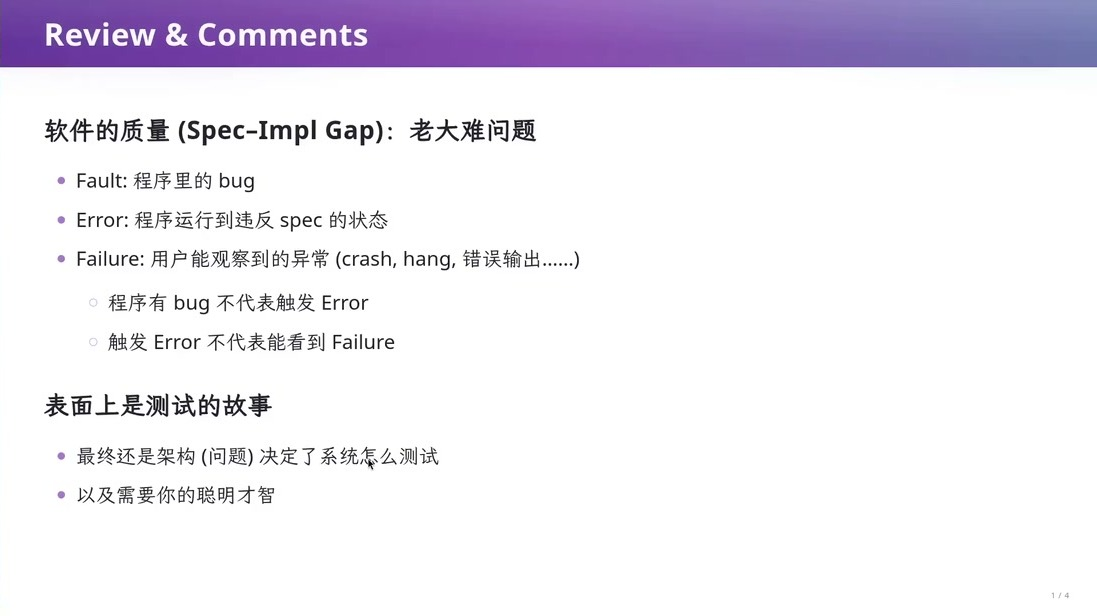
\includegraphics[width=0.88\textwidth]{figures/fig01_review_spec_impl_gap.jpg}
\caption{课程回顾：软件质量的 Spec--Impl Gap（Fault、Error、Failure 三阶段）与“表面上是测试的故事，最终还是架构决定了系统怎么测试”\vtag}
\label{fig:fig01_review_spec_impl_gap}
\end{figure}
\srcnote{00:00:15--00:02:00}

测试（Testing）试图构造刁钻的输入以触发隐藏的 Fault，断言（Specification-oriented Assertions）试图在内部状态刚刚偏离规约时立刻拉响警报，将潜伏的 Error 转化为显式的 Failure。然而，正如对应配图 下半部分所强调的：\textbf{表面上看，这似乎是一个关于“如何写测试用例”的故事；但剥开表象之后，真正决定一个软件系统好不好测、能不能测透的，依然是软件的底层架构（Architecture），以及人类工程师设计实验的聪明才智。}

为了直观说明架构对可测试性的决定性作用，我们可以回顾上一讲课堂现场演示的浏览器 3D 战术射击游戏（类 CS:GO 项目 \texttt{CS:THREE}）。表面上，玩家在屏幕上看到的是 Dust2 地图的光影、墙壁纹理与持枪角色动画；但如果一个游戏系统的架构设计合格，它的\textbf{底层游戏引擎（Game Engine）必须与图形渲染界面（Rendering UI）彻底解耦}。

在底层游戏引擎眼中，根本不存在像素或截图，整个游戏世界在任意离散时刻 $t$ 只是一个纯粹的数学状态向量 $s_t \in \mathcal{S}$：其中包含每颗子弹的三维空间坐标 $(x, y, z)$、速度向量 $\vec{v}$、武器类型（例如 AK-47 还是 AWP 的子弹）、各个角色的生命值、朝向与碰撞盒。每当逻辑时钟向前推进一帧（Tick），引擎根据当前状态 $s_t$ 以及该帧收集到的外部玩家指令序列 $a_t$（例如 \texttt{player 1 left key down}），通过一个完全确定性的状态转移函数 $f$ 计算出下一帧状态 $s_{t+1}$：
\begin{equation}
s_{t+1} = f(s_t, a_t), \qquad v_t^{(\text{role})} = \pi_{\text{role}}(s_t)
\label{eq:engine_state_projection}
\end{equation}
而屏幕上的画面，不过是投影函数 $\pi_{\text{role}}$ 将无图形的内部状态 $s_t$ 投射到特定观察者视角下的显示模型 $v_t^{(\text{role})}$：普通玩家通过 $\pi_{\text{player}}$ 看到受限的第一人称主视角，而比赛解说员（OB 视角）则通过 $\pi_{\text{OB}}$ 看到全局上帝视角；回放系统（Replay）也只需按序重放初始状态 $s_0$ 与指令流 $\{a_t\}$ 即可精确复现整场对局。

\begin{figure}[H]
\centering
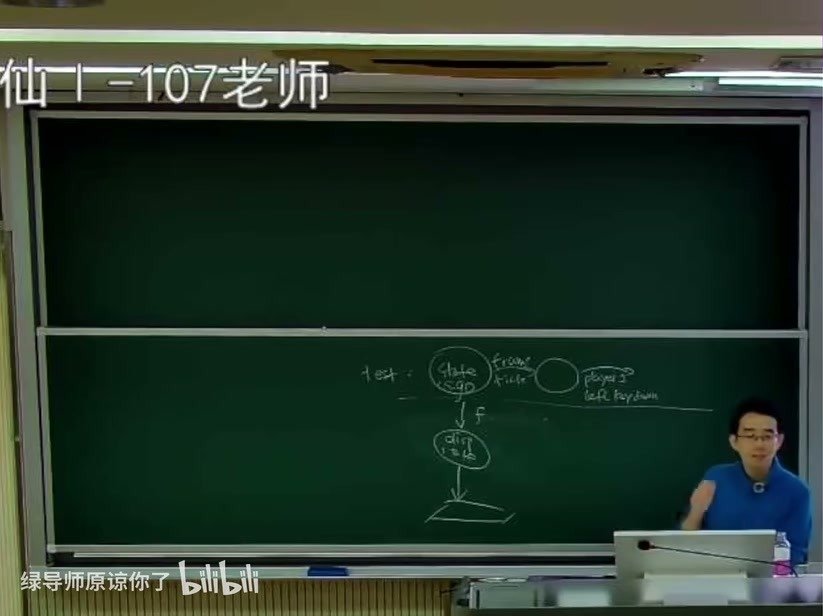
\includegraphics[width=0.72\textwidth]{figures/fig03_board_state_transition_test.jpg}
\caption{黑板板书：软件状态转移循环 $s_t \xrightarrow{f} s_{t+1}$ 与外部按键事件（如 \texttt{player 1 left key down}）驱动的无头（Headless）测试模型\vtag}
\label{fig:fig03_board_state_transition_test}
\end{figure}
\srcnote{00:05:20--00:06:30}

如对应配图 的黑板板书所示，\begin{practicebox}{架构设计准则：将游戏/系统核心状态机与渲染视图彻底分离}
在设计诸如 3D 射击游戏（\texttt{CS:THREE}）、GUI 编辑器或分布式存储引擎时，切忌将核心业务逻辑与像素渲染、DOM 操作或网络套接字直接耦合。应当将底层引擎设计为无头（Headless）、确定性的状态转移函数 $s_{t+1} = f(s_t, a_t)$，而将第一人称画面、OB 上帝视角与回放（Replay）统一实现为状态投影 $\pi_{\text{role}}(s_t)$。这样既能避免智能体在调试时因频繁截图耗尽上下文窗口，又能直接对状态机执行毫秒级高吞吐单元测试。
\end{practicebox}

一旦架构上实现了公式 \eqref{eq:engine_state_projection} 所示的“状态演化 $f$”与“视图投影 $\pi$”分离，测试就不再需要启动笨重的浏览器去一帧帧截图比对——要知道，在上一讲的轨迹复盘中，DeepSeek 智能体到了开发后期正是因为疯狂调用多机位截图，把海量 Base64 图像塞进上下文，白白烧光了 Token 额度并触发 \texttt{413 Payload Too Large} 错误。相反，只要引擎层是无头（Headless）且确定性的纯状态机，我们就可以在毫秒级时间内直接向 $f$ 注入成千上万组指令流 $\{a_t\}$，对弹道飞行、碰撞检测和伤害结算进行高吞吐的单元与重放测试。

\subsection{“合理”的测试目录分层及其在大型工程中的演化困境}

既然要把不同粒度的测试分开，如果我们直接向大模型（如 GPT 或 Claude）提问：“请为我的项目设计一套多层级测试目录结构”，大模型几乎会脱口而出一套教科书般“合理”的方案（对应配图）：

\begin{figure}[H]
\centering

\includegraphics[width=0.88\textwidth]{figures/fig02_testing_hierarchy_naive.jpg}
\caption{“合理”的测试分层：大模型给出的标准 \texttt{tests/\{unit,module,system\}} 目录结构与 \texttt{justfile} 入口，以及随之而来的多处维护困境\vtag}
\label{fig:fig02_testing_hierarchy_naive}
\end{figure}
\srcnote{00:02:05--00:05:15}

在这套标准方案中，项目根目录下除了源码目录 \texttt{src/}，还会建立 \texttt{tests/unit/}（单元测试）、\texttt{tests/module/}（模块测试）与 \texttt{tests/system/}（系统测试）三个子目录，并在根目录放一个 \texttt{justfile}（或者 \texttt{Makefile}）作为命令执行入口，提供诸如 \texttt{just test-unit}、\texttt{just test-system} 之类的快捷命令。

对于一个只有几千行代码、纯靠周末两天 Vibe Coding 攒出来发到 B 站博眼球的玩具项目来说，这种结构完全够用。但当项目规模增长到 \textbf{10万}行乃至向 \textbf{100万}行演进时，这种“目录即分类、脚本即入口”的组织方式就会暴露出致命的架构缺陷：
\begin{enumerate}
    \item \textbf{信息散落与交叉依赖（Cross-Dependency）}：假设团队现在需要新增一类依赖 QEMU 虚拟机的内核集成测试。在传统组织方式下，你需要同时修改几个地方？首先要在目录树里新建目录；其次要修改 \texttt{justfile} 增加执行配方；接着要修改 \texttt{.github/workflows/ci.yml} 把它加进持续集成流水线；可能还要修改 \texttt{.git/hooks/pre-commit} 决定提交前跑不跑它；最后还得更新开发文档告诉同事这个测试的存在。
    \item \textbf{智能体与人类的“部分更新”综合症}：一旦测试策略被拆散在目录名、\texttt{justfile}、CI YAML 配置和 Markdown 文档四五个地方，无论是人类开发者还是 AI Coding Agent，在后续迭代中都极易发生“改了 A 忘了改 B”的失步现象。更可怕的是，如果某个新写的测试目录漏加进了 \texttt{justfile} 或 CI 脚本，CI 流水线依然会一片绿灯（All Green），给人一种“所有测试全部通过”的虚假安全感！
\end{enumerate}

\subsection{把测试策略写进文档：\texttt{docs/testing.md} 与双向一致性核对}

如何从架构层面根治上述多处维护的顽疾？主讲教师展示了一种极具洞察力的工程设计：\textbf{拒绝将“人类阅读的文档”与“机器执行的配置”拆成两份文件，而是在 \texttt{docs/testing.md} 中直接维护一张结构化的 Markdown 表格，使其成为整个仓库测试策略的唯一事实来源（Single Source of Truth，SSOT）。}

\begin{figure}[H]
\centering
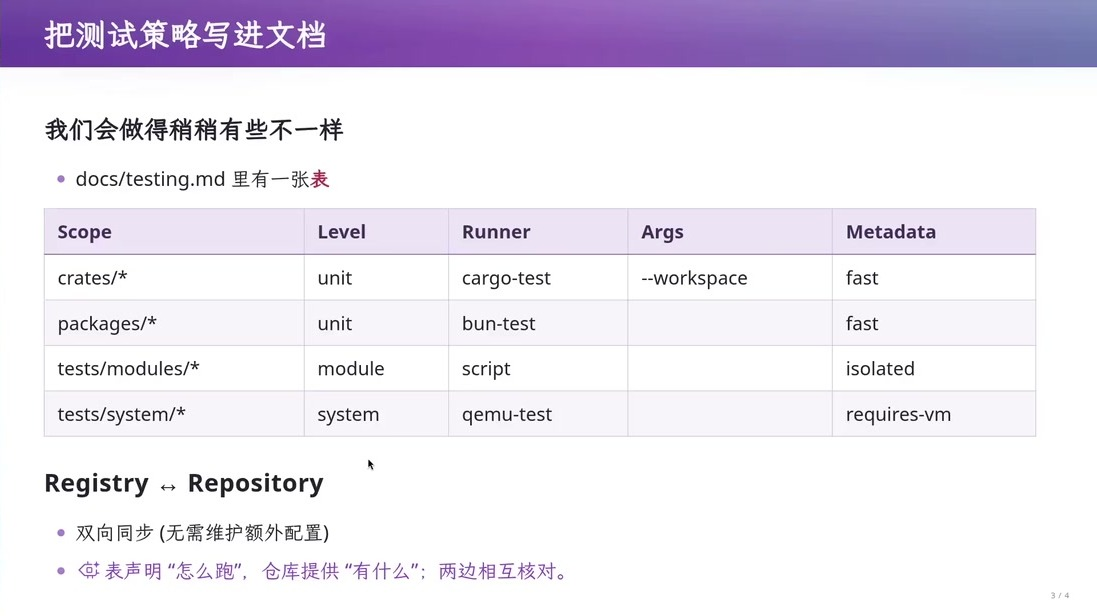
\includegraphics[width=0.88\textwidth]{figures/fig04_testing_md_ssot_table.jpg}
\caption{把测试策略写进文档：在 \texttt{docs/testing.md} 中用一张表格统一声明测试范围、层级、执行器、参数与元数据标签，并建立 \texttt{Registry $\leftrightarrow$ Repository} 双向核对\vtag}
\label{fig:fig04_testing_md_ssot_table}
\end{figure}
\srcnote{00:07:05--00:09:55}

如对应配图 与对应汇总表 所示，这张位于 \texttt{docs/testing.md} 中的注册表（Registry）包含五个正交的列属性：

\begin{table}[H]
\centering
\caption{\texttt{docs/testing.md} 中的测试策略唯一事实来源（SSOT）注册表示例}
\label{tab:testing_md_ssot}
\begin{tabular}{p{2.8cm}p{1.8cm}p{2.4cm}p{2.4cm}p{3.2cm}}
\toprule
\textbf{Scope} & \textbf{Level} & \textbf{Runner} & \textbf{Args} & \textbf{Metadata} \\
\midrule
\texttt{crates/*} & \texttt{unit} & \texttt{cargo-test} & \texttt{--workspace} & \texttt{fast} \\
\texttt{packages/*} & \texttt{unit} & \texttt{bun-test} & & \texttt{fast} \\
\texttt{tests/modules/*} & \texttt{module} & \texttt{script} & & \texttt{isolated} \\
\texttt{tests/system/*} & \texttt{system} & \texttt{qemu-test} & & \texttt{requires-vm} \\
\bottomrule
\end{tabular}
\end{table}

在这张表格中：
\begin{itemize}
    \item \textbf{\texttt{Scope}} 声明该条规则覆盖仓库中的哪些目录或通配路径；
    \item \textbf{\texttt{Level}} 声明测试所属的逻辑层级（如 \texttt{unit}、\texttt{module}、\texttt{system}）；
    \item \textbf{\texttt{Runner}} 与 \textbf{\texttt{Args}} 声明调用何种测试驱动器及命令行参数；
    \item \textbf{\texttt{Metadata}} 则以自定义标签（Tag）记录该测试的运行特征——例如 \texttt{fast}（秒级完成，适合挂载在每次 \texttt{pre-commit} 钩子中运行）、\texttt{isolated}（需要进程隔离环境）、\texttt{requires-vm}（依赖 QEMU 虚拟机，适合在 Merge Request 的完整 CI 阶段运行）。
\end{itemize}

\begin{figure}[H]
\centering
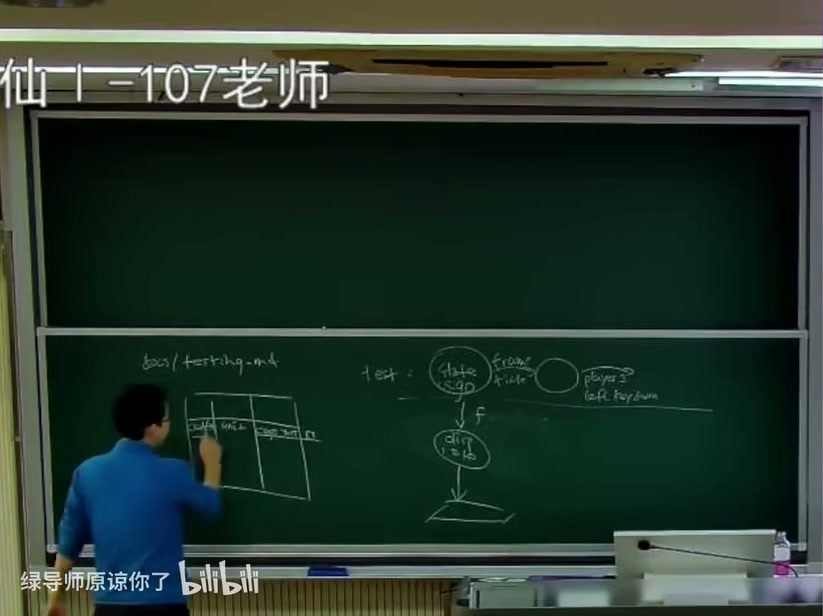
\includegraphics[width=0.72\textwidth]{figures/fig05_board_testing_registry_table.jpg}
\caption{黑板板书：左侧 \texttt{docs/testing.md} 注册表（Scope / Level / Runner / Tag）与右侧系统状态转移测试框架的映射关系\vtag}
\label{fig:fig05_board_testing_registry_table}
\end{figure}
\srcnote{00:08:20--00:09:45}

这种设计与 Donald Knuth 和 Silvio Levy 早年提出的文学编程系统 \textbf{CWEB}（从同一份源文件同时导出人类可读的排版文档与编译器可编译的 C 代码），以及现代工业界大型构建系统 \textbf{Bazel} 的声明式规则异曲同工（对应配图）。后台只需一个轻量级的解析器（“表格编译器”），就能直接读取 \texttt{docs/testing.md}，自动导出本地测试执行计划、Git \texttt{pre-commit} 检查脚本以及与特定平台解耦的 CI 流水线任务，彻底消除了多份配置文件之间的交叉同步负担。

\begin{figure}[H]
\centering
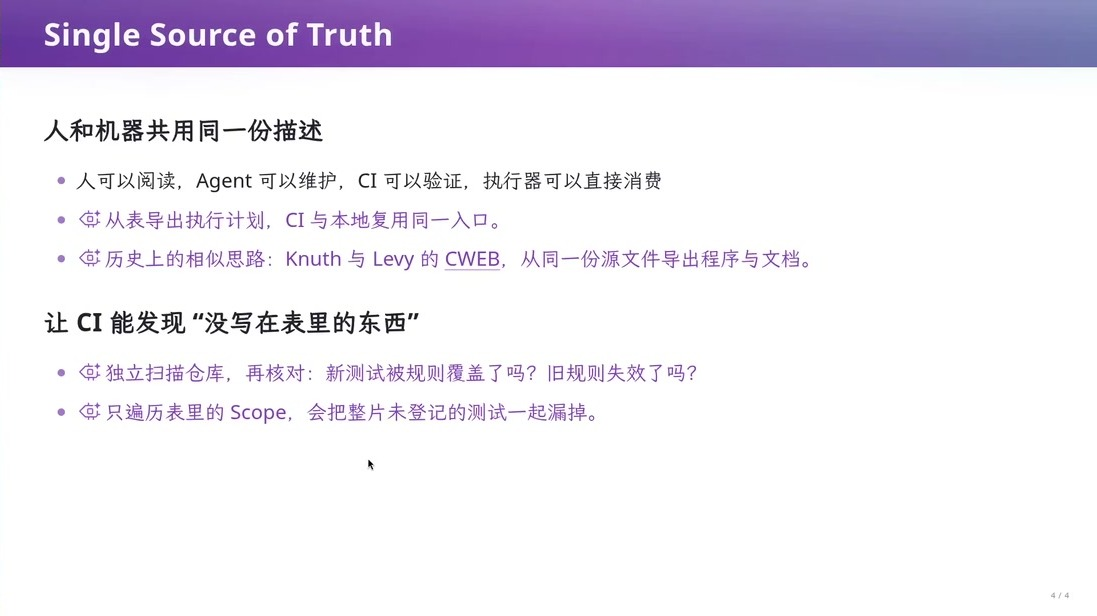
\includegraphics[width=0.88\textwidth]{figures/fig06_single_source_of_truth.jpg}
\caption{Single Source of Truth（唯一事实来源）：人机共用同一份描述，并通过独立扫描仓库与注册表双向比对，让 CI 揪出“没写在表里的东西”\vtag}
\label{fig:fig06_single_source_of_truth}
\end{figure}
\srcnote{00:10:00--00:12:30}

更进一步，如何防止智能体在仓库里新建了一个测试文件或测试目录，却忘了往 \texttt{docs/testing.md} 表格里登记？如果测试执行器仅仅顺着表格里的 \texttt{Scope} 去跑测试，那么未登记的测试就会成为“暗物质”——永远不被执行，也永远不会报错。为此，架构上必须引入 \textbf{\texttt{Registry $\leftrightarrow$ Repository} 双向一致性核对}。设注册表声明的规则集合所展开覆盖的测试目标集合为 $\mathcal{R}_{\text{doc}}$，而通过独立扫描代码仓库文件树（例如匹配所有 \texttt{*\_test.rs}、\texttt{*.spec.ts} 或 \texttt{tests/**} 下的测试脚本）发现的实际测试集合为 $\mathcal{T}_{\text{repo}}$，CI 的架构守卫（Architecture Guard）必须同时检验双向包含关系：
\begin{equation}
\mathcal{R}_{\text{doc}} \setminus \mathcal{T}_{\text{repo}} = \emptyset \quad (\text{无失效幽灵规则}), \qquad
\mathcal{T}_{\text{repo}} \setminus \mathcal{R}_{\text{doc}} = \emptyset \quad (\text{无未登记漏跑测试})
\label{eq:registry_repo_bijection}
\end{equation}

\begin{importantbox}{核心洞见：如何弥补 Coding Agent 的架构短板？}
大语言模型与 Coding Agent 擅长根据常见模式补全代码（例如生成标准的 \texttt{unit/module/system} 目录），但在面对“信息应当归属何处”“如何设计长程反馈机制防止静默退化”这类系统架构问题时往往缺乏主动性。弥补这一短板的方法，绝不是在 Prompt 里空洞地叮嘱一句“请你更聪明、更仔细一点”，而是\textbf{由人类工程师做出架构判断，将隐性的工程规范转化为机器可读取的唯一事实来源（\texttt{docs/testing.md}）与自动失败的双向一致性检查（公式 \eqref{eq:registry_repo_bijection}）}，从而把人类的架构智慧固化为 Agent 可以持续维护的闭环机制。
\end{importantbox}

% =========================================================================
% SECTION 2
% =========================================================================
\section{从运行程序到证明程序：形式化方法的历史源流与 Hoare 逻辑}

\subsection{为什么测试不够：从 Turing、McCarthy 到 Floyd 与 Hoare}

通过优良的测试架构与海量测试用例，我们可以不断找出软件中的 Bug 并修复它们。然而，正如 Edsger W. Dijkstra 在 \textbf{1970年}前后留下的那句振聋发聩的名言所指出的：
\begin{quote}
\textit{``Program testing can be used to show the presence of bugs, but never to show their absence!''}\\
（程序测试可以用来证明 Bug 的存在，但绝不能证明 Bug 的不存在！）
\end{quote}
哪怕你已经跑过了 $10,000$ 个测试用例且全部通过，程序依然可能在第 $10,001$ 个输入上崩溃。对于绝大多数日常软件，我们似乎已经默认“写出十万行绝对没有 Bug 的代码是不可能的”；但在人类计算机科学的黎明期，先驱们却怀抱着一个大胆得多的理想：\textbf{能不能不靠调试（Debugging），而是像初高中证明平面几何或代数定理那样，从数学上严格证明一个程序满足它的规格说明（Specification）？}

\begin{figure}[H]
\centering
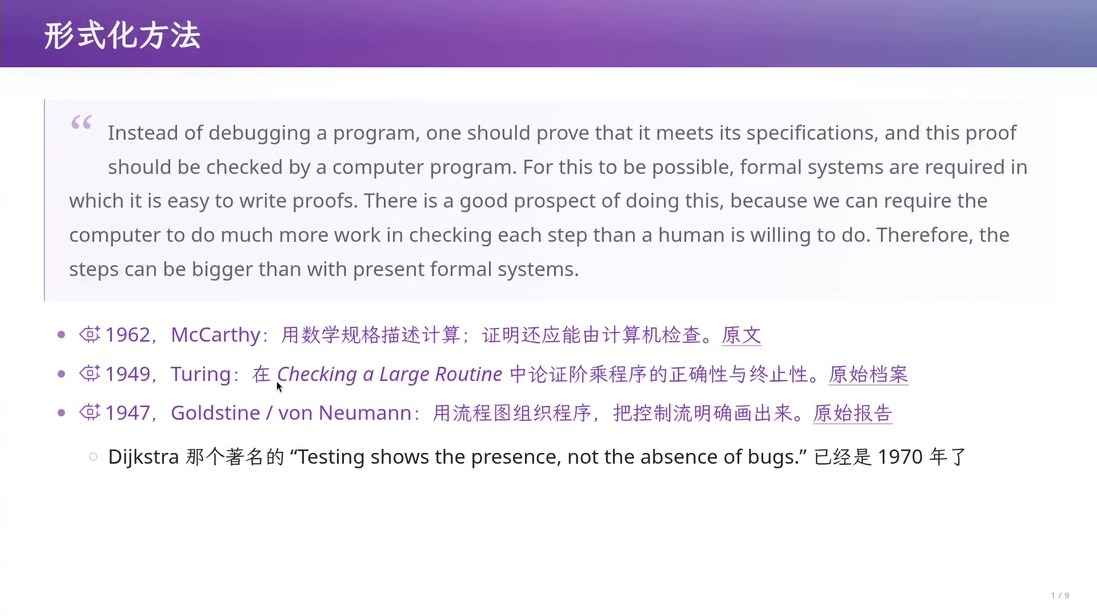
\includegraphics[width=0.88\textwidth]{figures/fig07_formal_methods_history_mccarthy_turing.jpg}
\caption{形式化方法的历史溯源：John McCarthy（1962年）、Alan Turing（1949年《Checking a Large Routine》）与 Goldstine--von Neumann（1947年）的开创性论述\vtag}
\label{fig:fig07_formal_methods_history_mccarthy_turing}
\end{figure}
\srcnote{00:12:33--00:15:45}

如对应配图 所示，这一思想几乎与现代电子计算机同龄：
\begin{itemize}
    \item \textbf{1947 年（Goldstine 与 von Neumann）}：在规划早期存储程序计算机的程序框图时，就已经尝试用数学断言标注控制流节点的状态性质；
    \item \textbf{1949 年（Alan Turing）}：在剑桥大学会议论文《Checking a Large Routine》中首次明确讨论了如何通过在程序关键位置插入数学断言来检验一个大型子程序的正确性与终止性；
    \item \textbf{1962年（John McCarthy）}：在经典论文中写下了极具前瞻性的纲领——
    \begin{quote}
    \textit{``Instead of debugging a program, one should prove that it meets its specifications, and this proof should be checked by a computer program. For this to be possible, formal systems are required in which it is easy to write proofs. There is a good prospect of doing this, because we can require the computer to do much more work in checking each step than a human is willing to do.''}
    \end{quote}
    McCarthy 不仅提出“应当证明程序符合规格而非调试程序”，更一针见血地指出：\textbf{这份数学证明本身也应当交给计算机程序去检查！}因为计算机不知疲倦，可以为每一步推理执行远超人类耐心的机械核验。
\end{itemize}

为什么数学家们坚信程序可以被严格证明？因为在离散数学与数理逻辑中，一切复杂的数学大厦都可以建立在极其简洁的公理系统之上。例如，\textbf{皮亚诺算术（Peano Arithmetic）}仅需两条生成规则即可递归定义整个自然数集合 $\mathbb{N}$：
\begin{equation}
\text{基础公理： } 0 \in \mathbb{N}, \qquad
\text{归纳生成规则： } \forall n\; (n \in \mathbb{N} \implies S(n) = n + 1 \in \mathbb{N})
\label{eq:peano_axioms}
\end{equation}
在公式 \eqref{eq:peano_axioms} 中，我们不过是把 $0+1$ 记作十进制符号 $1$（或二进制符号 $1_2$），把 $0+1+1$ 记作十进制符号 $2$（或二进制符号 $10_2$）。在此基础上，我们可以递归定义加法、乘法，并严格证明诸如完全平方公式之类的代数恒等式（其中包含一次项 \textbf{2x}）：
\begin{equation}
\forall x \in \mathbb{N}:\quad x^2 + 2x + 1 = (x + 1)^2
\label{eq:algebra_identity_2x}
\end{equation}

\begin{figure}[H]
\centering
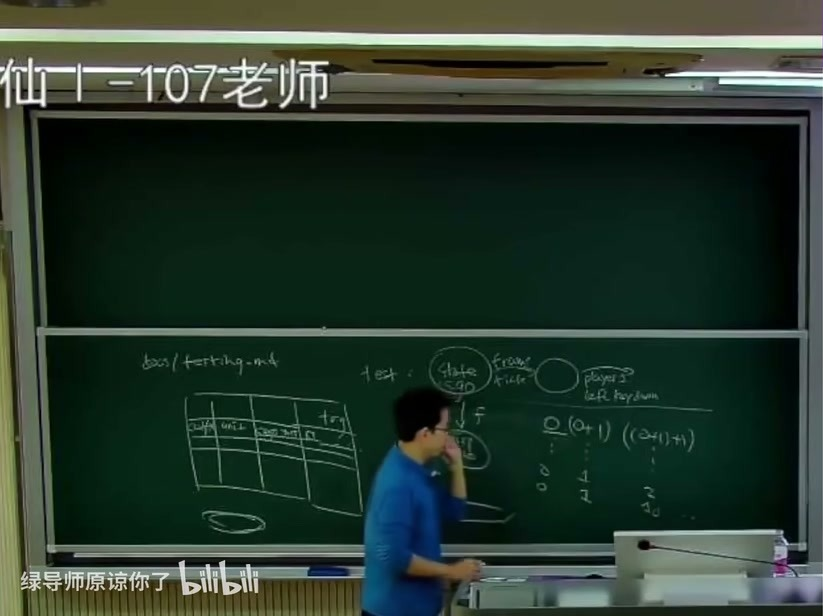
\includegraphics[width=0.72\textwidth]{figures/fig08_board_program_proof_formula.jpg}
\caption{黑板板书：从皮亚诺自然数公理与数学归纳法 $Q(n) \Rightarrow Q(n+1)$ 出发，将程序执行状态纳入形式化演绎推理\vtag}
\label{fig:fig08_board_program_proof_formula}
\end{figure}
\srcnote{00:15:50--00:16:35}

既然自然数和代数运算可以通过公理化方法严格推理（对应配图），那么由明确指令构成的计算机程序为什么不能？\textbf{1967 年，Robert W. Floyd} 在《Assigning Meanings to Programs》中系统提出了在控制流图（Flowchart）的边上附加逻辑断言、由局部转换正确性推导整体正确性的方法；紧接着在 \textbf{1969 年，C. A. R. (Tony) Hoare} 发表了流芳百世的奠基性论文《An Axiomatic Basis for Computer Programming》（对应配图），正式确立了程序公理化推理的语法与规则体系——即 \textbf{Hoare 逻辑（Hoare Logic）}。

\begin{figure}[H]
\centering
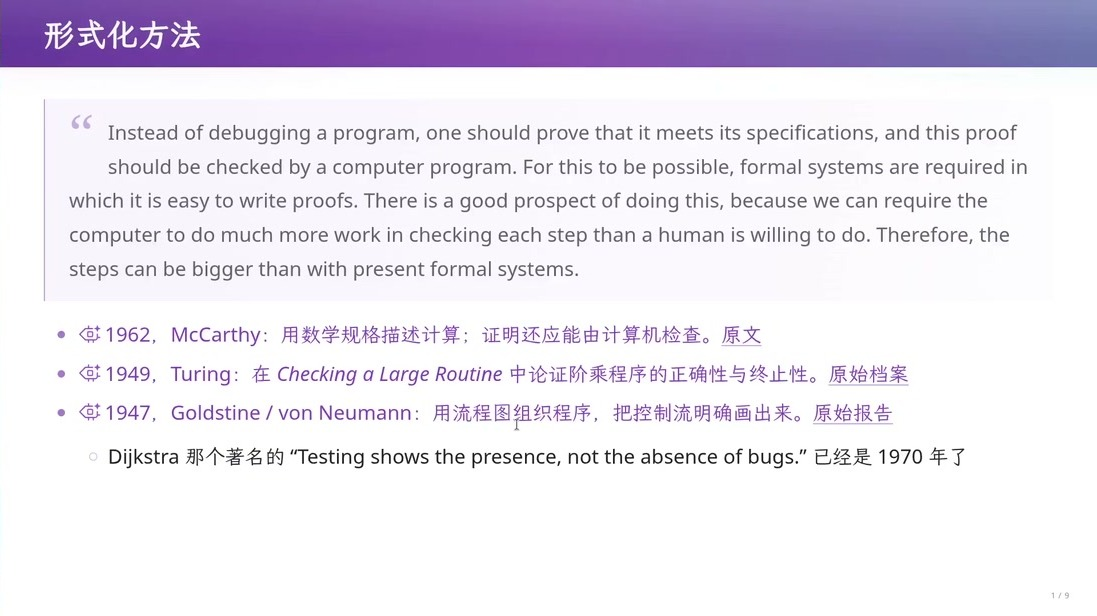
\includegraphics[width=0.88\textwidth]{figures/fig09_formal_methods_floyd_hoare.jpg}
\caption{形式化方法先驱：Floyd（1967 年控制流断言）与 Hoare（1969 年《An Axiomatic Basis for Computer Programming》）\vtag}
\label{fig:fig09_formal_methods_floyd_hoare}
\end{figure}
\srcnote{00:16:40--00:17:20}

\subsection{文献精读：Hoare（1969）对机器算术边界的公理化洞察}

在课堂上，主讲教师直接打开了 Hoare 1969 年原始论文的全文（对应配图 与对应配图）。Hoare 在引言中开宗明义地写道：
\begin{quote}
\textit{``Computer programming is an exact science in that all the properties of a program and all the consequences of executing it in any given environment can, in principle, be found out from the text of the program itself by means of purely deductive reasoning.''}
\end{quote}

尤为精彩的是论文第 2 节（\textit{Computer Arithmetic}）：Hoare 敏锐地提醒读者，在证明程序性质之前，必须先搞清楚底层机器算术遵循的究竟是哪套公理！数学上的整数集合 $\mathbb{Z}$ 是无限的，但真实计算机寄存器里的整数却存在严格的上界 $M$（在论文 Table II 的微型示例中取边界值 $B = 3$，即仅能表示集合 $\{0, 1, 2, 3\}$）。

\begin{figure}[H]
\centering
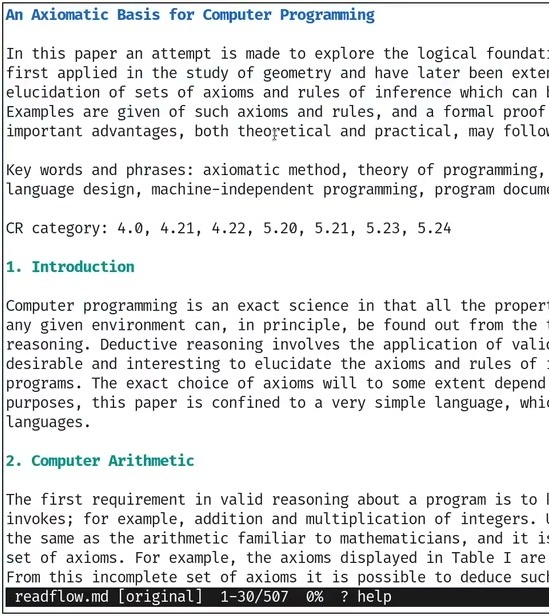
\includegraphics[width=0.78\textwidth]{figures/fig10_hoare_1969_paper_text.jpg}
\caption{文献精读（一）：Hoare（1969）《An Axiomatic Basis for Computer Programming》引言与算术公理探讨\vtag}
\label{fig:fig10_hoare_1969_paper_text}
\end{figure}
\srcnote{00:17:25--00:17:50}

\begin{figure}[H]
\centering
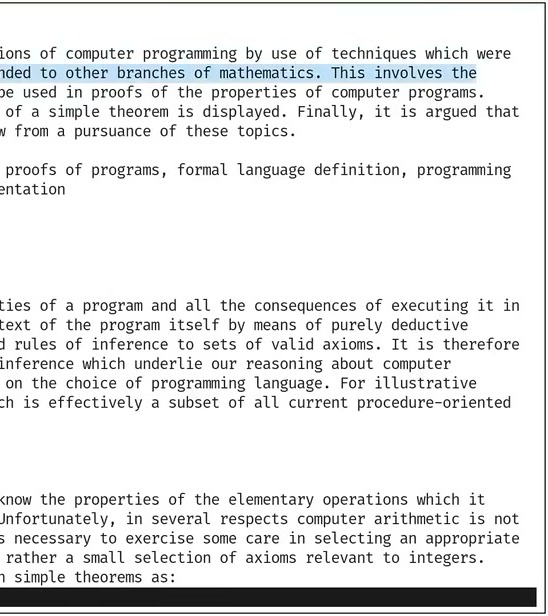
\includegraphics[width=0.78\textwidth]{figures/fig11_hoare_1969_modular_arithmetic_table.jpg}
\caption{文献精读（二）：Hoare（1969）论文 Table II 展示有界整数 $\{0,1,2,3\}$ 的三种加乘语义解释（Strict、Firm Boundary、Modulo）\vtag}
\label{fig:fig11_hoare_1969_modular_arithmetic_table}
\end{figure}
\srcnote{00:17:50--00:18:15}

当算术运算结果超出机器表示上界 $B$ 时，Hoare 指出了三种截然不同的形式化语义解释（对应配图b）：
\begin{enumerate}
    \item \textbf{严格解释（Strict Interpretation）}：凡是超出 $\{0, 1, \dots, B\}$ 范围的运算结果均视为不存在（未定义或直接触发溢出陷阱，表中记作 `?`）；
    \item \textbf{饱和边界解释（Firm Boundary）}：溢出结果被截断（Clamp）在最大边界值 $B$ 上；
    \item \textbf{模运算解释（Modulo Arithmetic）}：结果对 $B+1$ 取模回绕（Wrap-around）。
\end{enumerate}
用数学公式表示，在边界 $B$（如 $B=3$ 或 $B=2^{32}-1$）下，后两种算术的加法语义分别为：
\begin{equation}
a \boxplus_{[0,B]} b = \min(a + b,\, B) \quad (\text{Firm Boundary}), \qquad
a \oplus_{B+1} b = (a + b) \bmod (B + 1) \quad (\text{Modulo Arithmetic})
\label{eq:hoare_bounded_arithmetic}
\end{equation}
例如在模 $4$ 算术下，$2 \oplus_4 3 = 1$；而在饱和算术下，$2 \boxplus_{[0,3]} 3 = 3$。如果脱离了公式 \eqref{eq:hoare_bounded_arithmetic} 的精确语义，盲目套用理想数学整数的定律（如“$x + 1 > x$ 恒成立”），在遇到机器整数溢出时就会得出完全错误的证明！

\subsection{Hoare 三元组 $\{P\}\; C\; \{Q\}$：部分正确性与总正确性}

为了给一段程序写下可推导的形式化规约（Formal Specification），Hoare 引入了著名的 \textbf{Hoare 三元组（Hoare Triple）}记号（对应配图）：
\begin{equation}
\{P\} \;\; C \;\; \{Q\}
\label{eq:hoare_triple_basic}
\end{equation}
其中：
\begin{itemize}
    \item $P$ 称为\textbf{前置条件（Precondition）}，是对程序执行前初始状态 $s$ 的逻辑断言；
    \item $C$ 是待执行的\textbf{程序或语句（Command / Program）}；
    \item $Q$ 称为\textbf{后置条件（Postcondition）}，是对程序执行结束后终止状态 $s'$ 的逻辑断言。
\end{itemize}

\begin{figure}[H]
\centering
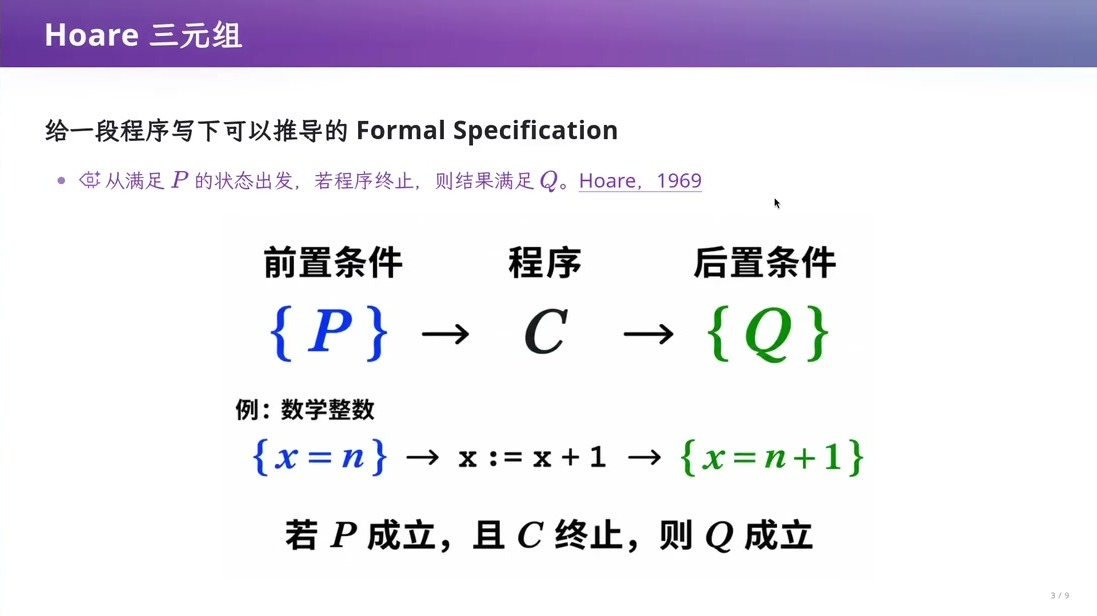
\includegraphics[width=0.88\textwidth]{figures/fig12_hoare_triple_slide.jpg}
\caption{Hoare 三元组 $\{P\} \to C \to \{Q\}$：前置条件、程序与后置条件的形式化定义及数学整数赋值示例\vtag}
\label{fig:fig12_hoare_triple_slide}
\end{figure}
\srcnote{00:18:20--00:20:45}

例如，在理想数学整数语义下，如果前置条件是 $\{x = n\}$（例如 $x = 4$），执行赋值语句 $C \equiv (\texttt{x := x + 1})$ 后，后置条件 $\{x = n + 1\}$（即 $x = 5$）必然成立。但在这里，有一处极其关键的逻辑细节绝不能含糊带过——那就是\textbf{“如果程序 $C$ 执行终止”}！根据是否要求程序一定终止，程序正确性严格划分为两类：
\begin{align}
\models_{\text{part}} \{P\}\; C\; \{Q\} &\iff \forall s, s' \in \mathcal{S}:\; \big(s \models P \;\land\; \langle C, s \rangle \Downarrow s'\big) \implies s' \models Q \label{eq:partial_correctness} \\
\models_{\text{tot}} \{P\}\; C\; \{Q\} &\iff \forall s \in \mathcal{S}:\; s \models P \implies \big(\exists s' \in \mathcal{S}:\; \langle C, s \rangle \Downarrow s' \;\land\; s' \models Q\big) \label{eq:total_correctness}
\end{align}
在公式 \eqref{eq:partial_correctness} 与 \eqref{eq:total_correctness} 中，$\langle C, s \rangle \Downarrow s'$ 表示程序 $C$ 从状态 $s$ 出发经有限步执行后正常终止于状态 $s'$：
\begin{itemize}
    \item \textbf{部分正确性（Partial Correctness，公式 \eqref{eq:partial_correctness}）}：仅承诺“\textbf{一旦}程序终止，结果一定满足 $Q$”。换言之，如果一个排序程序进入死循环 `\texttt{while (true) ;}` 永远不返回，它在部分正确性意义下竟然是“满足任何后置条件 $Q$”的（因为蕴含式的前提 $\langle C, s \rangle \Downarrow s'$ 为假，整个蕴含式恒真）！
    \item \textbf{总正确性（Total Correctness，公式 \eqref{eq:total_correctness}）}：等于“部分正确性 $+$ 终止性（Termination）”，要求从任何满足 $P$ 的状态出发，程序 $C$ 不仅必须在有限步内停机，而且停机状态满足 $Q$。
\end{itemize}

\begin{warningbox}{关键辨析：部分正确性（Partial Correctness）不保证程序终止！}
在阅读或书写 Hoare 三元组 $\{P\}\; C\; \{Q\}$ 时，绝不能偷偷忽略“若程序 $C$ 终止”这一前提条件。在部分正确性语义（公式 \eqref{eq:partial_correctness}）下，一个包含死循环 \texttt{while (true) ;}、永远不返回的排序程序，竟然在逻辑上满足任何后置条件 $Q$！因此，工业级高可靠验证必须进一步引入良基关系或递减秩函数（Ranking Function / Variant），将部分正确性提升为包含停机保证的总正确性（Total Correctness，公式 \eqref{eq:total_correctness}）。
\end{warningbox}

有了 Hoare 三元组，顺序执行的程序就可以通过\textbf{赋值公理（Assignment Axiom）}与\textbf{顺序组合规则（Sequential Composition Rule）}像多米诺骨牌一样串联推导：
\begin{equation}
\frac{}{\{Q[E/x]\}\;\; \texttt{x := E}\;\; \{Q\}} \;(\text{Assign}), \qquad
\frac{\{P\}\;\; C_1\;\; \{R\} \qquad \{R\}\;\; C_2\;\; \{Q\}}{\{P\}\;\; C_1;\, C_2\;\; \{Q\}} \;(\text{Seq})
\label{eq:hoare_assign_seq}
\end{equation}
其中 $Q[E/x]$ 表示将后置条件 $Q$ 中所有的自由变量 $x$ 替换为表达式 $E$。例如要使执行 `\texttt{x := x + 1}` 后满足 $x > 0$，只需前置状态满足 $(x+1) > 0$（即 $x \ge 0$）。

% =========================================================================
% SECTION 3
% =========================================================================
\section{一个不变式抵过无数次运行：循环不变式与 Boyer--Moore 多数投票算法}

\subsection{循环不变式（Loop Invariant）的三步推理规则}

顺序语句与条件分支都很容易用有限步逻辑推理串起来，但\textbf{循环（Loop）}是程序证明中最棘手的拦路虎：一段 `\texttt{while (B) C}` 循环在运行时可能执行 $10$ 次、$10^6$ 次甚至任意多次，我们怎么可能用静态的、有限长度的数学证明去概括动态的、任意多轮的循环执行？

Floyd 与 Hoare 给出的答案是寻找一个\textbf{循环不变式（Loop Invariant）}——即一个在循环开始前成立、且每执行完一轮循环体 $C$ 后依然保持成立的逻辑命题 $I$（对应配图）。

\begin{figure}[H]
\centering
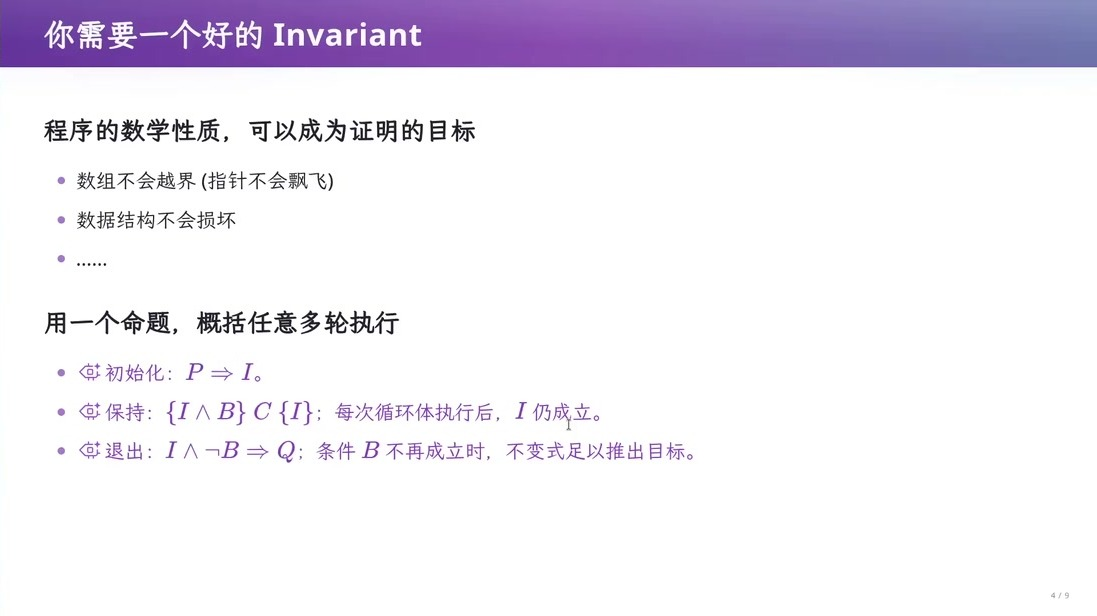
\includegraphics[width=0.88\textwidth]{figures/fig13_loop_invariant_slide.jpg}
\caption{你需要一个好的 Invariant：程序的数学性质（数组不越界、数据结构不损坏）与循环不变式的初始化、保持、退出三步推理\vtag}
\label{fig:fig13_loop_invariant_slide}
\end{figure}
\srcnote{00:20:50--00:22:30}

具体而言，要证明三元组 $\{P\}\; \texttt{while (B) C}\; \{Q\}$（在部分正确性意义下），我们需要找到一个命题 $I$，并完成以下三步证明（公式 \eqref{eq:loop_invariant_rules}）：
\begin{equation}
\begin{cases}
\textbf{1. 初始化（Initialization）：} & P \implies I \\[4pt]
\textbf{2. 保持（Preservation / Maintenance）：} & \{I \land B\}\;\; C\;\; \{I\} \\[4pt]
\textbf{3. 退出（Exit / Consequence）：} & (I \land \neg B) \implies Q
\end{cases}
\label{eq:loop_invariant_rules}
\end{equation}
写成自然演绎推理规则的形式即为：
\begin{equation}
\frac{P \implies I \qquad \{I \land B\}\;\; C\;\; \{I\} \qquad I \land \neg B \implies Q}{\{P\}\;\; \texttt{while (B) do C}\;\; \{Q\}} \;(\text{While})
\label{eq:hoare_while_rule}
\end{equation}

如对应配图 的黑板板书所示，公式 \eqref{eq:loop_invariant_rules} 的直觉非常清晰：只要进入循环前 $I$ 成立（初始化），且每次在循环条件 $B$ 为真时跑完一圈循环体 $C$ 都能让 $I$ 继续成立（保持），那么无论循环在运行时转了 $0$ 圈、$100$ 圈还是 $10^9$ 圈，只要它最终跳出循环，在跳出那一刻我们就同时拥有两条铁证：\textbf{不变式 $I$ 依然成立，且循环条件 $B$ 已经变为假（$\neg B$）}！用 $I \land \neg B$ 即可一步推出目标性质 $Q$。

\begin{figure}[H]
\centering
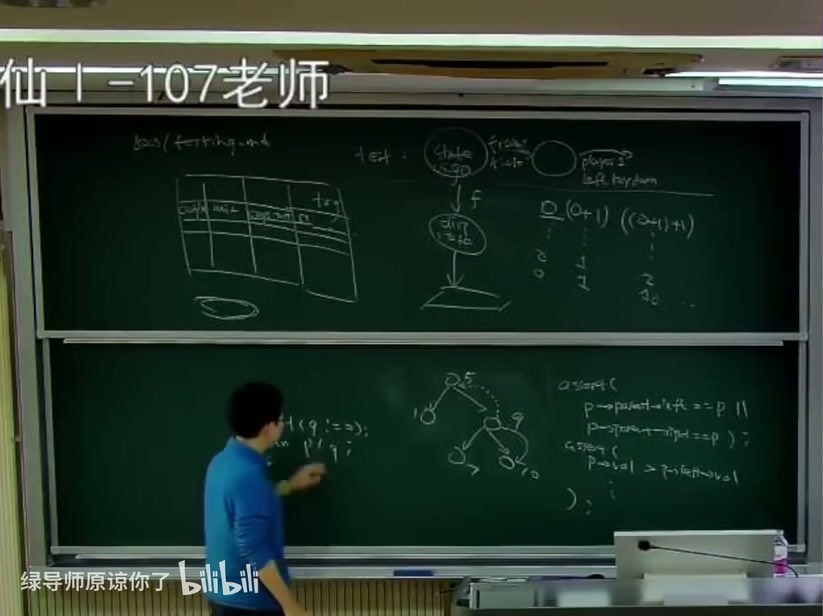
\includegraphics[width=0.72\textwidth]{figures/fig14_board_loop_invariant_assert.jpg}
\caption{黑板板书：在 \texttt{while (cond)} 循环退出点插入 \texttt{assert(!cond)}，以及平衡二叉搜索树（BST）旋转中的父子指针断言\vtag}
\label{fig:fig14_board_loop_invariant_assert}
\end{figure}
\srcnote{00:22:35--00:25:15}

在工程实践中，数据结构的不变式与代码里的运行时断言（\texttt{assert}）是一体两面的。主讲教师在黑板上画了一棵带 \texttt{parent} 指针的平衡二叉搜索树（Balanced Binary Search Tree，例如红黑树或 AVL 树，对应配图 右下角）：凡是亲手写过不抄书的红黑树旋转（Rotation）的同学都知道，在左旋、右旋更新指针的过程中，极其容易把某个节点的 \texttt{parent} 指针指飞，导致树结构被拉坏。如果我们把“一棵合法带父指针二叉搜索树”的数学不变式 $\mathcal{I}_{\text{BST}}(T)$ 显式写出来：
\begin{equation}
\begin{aligned}
\mathcal{I}_{\text{BST}}(T) \;\triangleq\; \forall p \in T:\;
&\big(p.\mathit{left} \neq \mathsf{null} \implies p.\mathit{left}.\mathit{parent} = p \;\land\; p.\mathit{left}.\mathit{val} < p.\mathit{val}\big) \\
\land\; &\big(p.\mathit{right} \neq \mathsf{null} \implies p.\mathit{right}.\mathit{parent} = p \;\land\; p.\mathit{right}.\mathit{val} > p.\mathit{val}\big)
\end{aligned}
\label{eq:bst_invariant}
\end{equation}
那么在测试时，公式 \eqref{eq:bst_invariant} 就是我们在每次旋转操作前后调用的检查函数 `\texttt{assert(p->parent->left == p || p->parent->right == p)}`；而在形式化验证中，公式 \eqref{eq:bst_invariant} 就是我们要用定理证明器证明“旋转操作保持不变”的目标命题！\begin{knowledgebox}{从运行时 Assertion 到静态 Invariant：同一数学性质的两种生命形态}
程序员在 C/Rust 代码里写下的 \texttt{assert(p->parent->left == p || p->parent->right == p)}，与形式化验证专家在定理证明器里写下的结构不变式 $\mathcal{I}_{\text{BST}}(T)$（公式 \eqref{eq:bst_invariant}），本质上是同一个数学命题在不同验证阶段的体现：动态断言在单次运行的当前状态上做抽样检验（$\mathcal{O}(1)$ 触发局部观察），而静态不变式证明则通过归纳法一次性覆盖未来所有可能的执行轨迹。
\end{knowledgebox}

此外，像“指针解引用永不为空（$\mathit{ptr} \neq \mathsf{null}$）”“数组下标永不越界（$0 \le i < \mathit{len}$）”“除法指令 `\texttt{return p / q}` 中分母永不为零（$q \neq 0$）”等隐式安全要求，本质上也都是程序每一行语句自带的断言命题。

\subsection{经典案例推导：Boyer--Moore 多数投票算法的循环不变式}

然而，\textbf{“写下代码很容易，找到能证明它正确的循环不变式却可能难如登天！”}为了让大家切身体会寻找不变式的智力门槛，主讲教师给出了 \textbf{1980年}由 Robert S. Boyer 与 J Strother Moore 提出的著名\textbf{多数投票算法（Boyer--Moore Majority Vote Algorithm）}——有趣的是，Boyer 和 Moore 当年提出这个算法，恰恰是为了给容错系统形式化验证“多数表决”性质！（对应配图）

\begin{figure}[H]
\centering
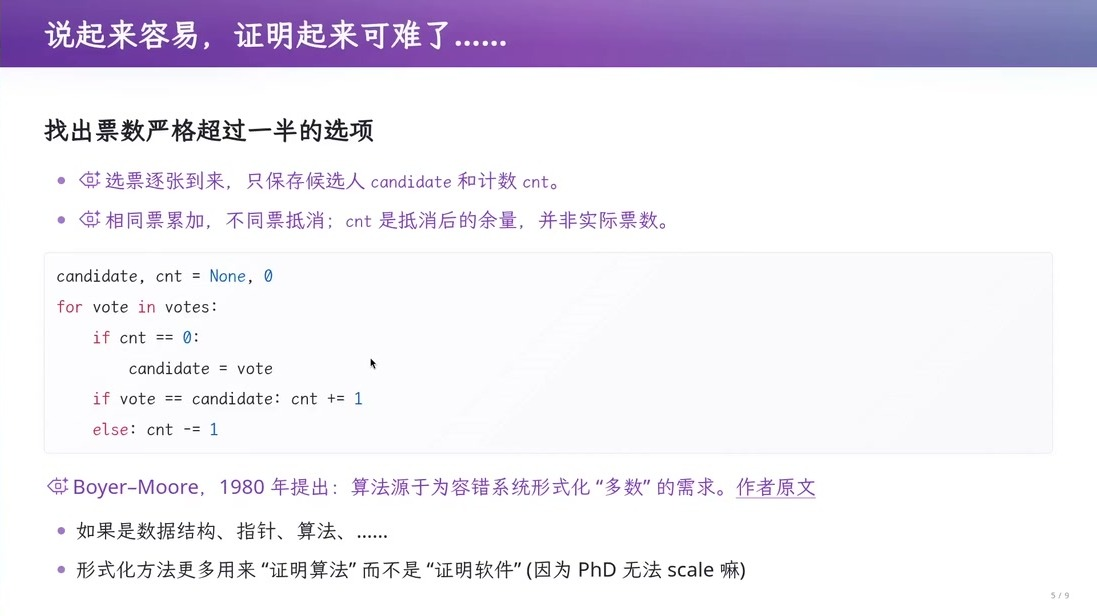
\includegraphics[width=0.88\textwidth]{figures/fig15_boyer_moore_majority_vote.jpg}
\caption{说起来容易，证明起来可难了：Boyer--Moore（1980年）多数投票算法的 9 行 Python 代码与“抵消后余量”循环不变式\vtag}
\label{fig:fig15_boyer_moore_majority_vote}
\end{figure}
\srcnote{00:25:20--00:28:40}

问题描述如下：给定一个长度为 $N$ 的选票序列 $\mathit{votes} = [v_1, v_2, \dots, v_N]$，已知其中存在一个严格多数选项 $c^*$（即投给 $c^*$ 的票数严格大于 $N/2$）。如何只遍历一遍序列、且仅使用两个标量变量（当前候选人 \texttt{candidate} 与计数器 \texttt{cnt}，空间复杂度 $\mathcal{O}(1)$）就找出这个多数选项 $c^*$？Boyer--Moore 算法的代码短得惊人：

\begin{lstlisting}[language=Python, caption={Boyer--Moore 多数投票算法核心实现}]
candidate, cnt = None, 0
for vote in votes:
    if cnt == 0:
        candidate = vote
    if vote == candidate:
        cnt += 1
    else:
        cnt -= 1
\end{lstlisting}

这段代码只有短短几行，但它之所以极难证明，是因为\textbf{程序在运行过程中是有损的（Lossy）}：它把过去读过的所有历史选票信息全部丢掉了，只留下手头的一个名字 \texttt{candidate} 和一个整数 \texttt{cnt}。更关键的是，\texttt{cnt} 根本不是 \texttt{candidate} 的真实得票数！那我们凭什么断言循环结束时留下的 \texttt{candidate} 一定是严格多数 $c^*$？

\begin{knowledgebox}{严格推导：Boyer--Moore 多数投票算法的循环不变式与正确性证明}
设前 $k$ 步已经读取的选票前缀多重集为 $S_k = \{v_1, v_2, \dots, v_k\}$（$0 \le k \le N$）。该算法真正的核心循环不变式 $I(k)$ 是：
\begin{quote}
\textbf{不变式 $I(k)$}：已读取的前 $k$ 张选票多重集 $S_k$，总可以划分为两部分：（1）$m_k$ 对\textbf{两个选项互不相同}的选票配对集合 $P_k = \{(a_1, b_1), \dots, (a_{m_k}, b_{m_k})\}$（其中每个配对满足 $a_j \neq b_j$）；以及（2）剩余的 $\mathit{cnt}_k$ 张\textbf{全部投给当前 $\mathit{candidate}_k$} 的选票多重集 $U_k$。
\end{quote}
写成精确的数学关系式即为：
\begin{equation}
\begin{aligned}
I(k) \;\triangleq\; &\big(\mathit{cnt}_k \ge 0 \;\land\; k = 2m_k + \mathit{cnt}_k\big) \\
&\land\; \forall x:\; \mathrm{count}(x, S_k) = \sum_{j=1}^{m_k} \big(\mathbb{I}[a_j = x] + \mathbb{I}[b_j = x]\big) + \mathit{cnt}_k \cdot \mathbb{I}[\mathit{candidate}_k = x]
\end{aligned}
\label{eq:boyer_moore_invariant}
\end{equation}

我们按照公式 \eqref{eq:loop_invariant_rules} 的三步法验证 $I(k)$：
\begin{enumerate}
    \item \textbf{初始化（$k = 0$）}：尚未读取任何选票时，$S_0 = \emptyset$，$m_0 = 0$，$\mathit{cnt}_0 = 0$，划分自然成立，故 $I(0)$ 为真。
    \item \textbf{保持（从 $k$ 到 $k+1$）}：假设处理完前 $k$ 张票后 $I(k)$ 成立，现在读入第 $k+1$ 张票 $v = v_{k+1}$，分三种情形讨论：
    \begin{itemize}
        \item \textbf{情形 A（$\mathit{cnt}_k = 0$）}：代码先执行 `\texttt{candidate = v}`，再执行 `\texttt{cnt += 1}`。此时令 $m_{k+1} = m_k$，$\mathit{candidate}_{k+1} = v$，$\mathit{cnt}_{k+1} = 1$，新票 $v$ 单独构成剩余票集合 $U_{k+1}$，配对集合 $P_{k+1} = P_k$ 不变，$I(k+1)$ 成立。
        \item \textbf{情形 B（$\mathit{cnt}_k > 0$ 且 $v = \mathit{candidate}_k$）}：代码执行 `\texttt{cnt += 1}`。此时令 $m_{k+1} = m_k$，$\mathit{cnt}_{k+1} = \mathit{cnt}_k + 1$，新票 $v$ 直接并入全部属于 $\mathit{candidate}_k$ 的剩余票集合 $U_{k+1}$，$I(k+1)$ 成立。
        \item \textbf{情形 C（$\mathit{cnt}_k > 0$ 且 $v \neq \mathit{candidate}_k$）}：代码执行 `\texttt{cnt -= 1}`。由于 $\mathit{cnt}_k \ge 1$，我们从剩余票集合 $U_k$ 中抽出一张属于 $\mathit{candidate}_k$ 的选票，与当前这张不同选项的新票 $v$ 配成一对 $(\mathit{candidate}_k, v)$（满足两者选项不同！）加入配对集合 $P_{k+1}$。此时配对数 $m_{k+1} = m_k + 1$，剩余票数 $\mathit{cnt}_{k+1} = \mathit{cnt}_k - 1 \ge 0$，且总票数 $2(m_k + 1) + (\mathit{cnt}_k - 1) = 2m_k + \mathit{cnt}_k + 1 = k + 1$，$I(k+1)$ 依然严格成立！
    \end{itemize}
    \item \textbf{退出（$k = N$）与严格多数性质推导}：当全部 $N$ 张票读完退出循环时，$I(N)$ 成立。设真正得票严格超过半数的选项为 $c^*$，即 $\mathrm{count}(c^*, S_N) > N / 2$。考察那 $m_N$ 对不同选项的选票配对 $(a_j, b_j)$：由于 $a_j \neq b_j$，\textbf{每一对配对中至多只能包含一张投给 $c^*$ 的票}，即 $\forall j:\; \mathbb{I}[a_j = c^*] + \mathbb{I}[b_j = c^*] \le 1$。代入公式 \eqref{eq:boyer_moore_invariant} 可得：
    \begin{equation}
    \frac{N}{2} < \mathrm{count}(c^*, S_N) \le m_N + \mathit{cnt}_N \cdot \mathbb{I}[\mathit{candidate}_N = c^*]
    \label{eq:boyer_moore_exit_bound}
    \end{equation}
    又因为 $N = 2m_N + \mathit{cnt}_N$，即 $m_N = \frac{N - \mathit{cnt}_N}{2}$，代入公式 \eqref{eq:boyer_moore_exit_bound} 两边同减 $m_N$ 得：
    \begin{equation}
    \mathit{cnt}_N \cdot \mathbb{I}[\mathit{candidate}_N = c^*] > \frac{N}{2} - m_N = \frac{\mathit{cnt}_N}{2} \ge 0
    \label{eq:boyer_moore_conclusion}
    \end{equation}
    公式 \eqref{eq:boyer_moore_conclusion} 左端严格大于 $0$，这同时强制推出了两个结论：第一，$\mathit{cnt}_N > 0$；第二，$\mathbb{I}[\mathit{candidate}_N = c^*] = 1$，即最终留下的 $\mathit{candidate}_N = c^*$ 必然是那个严格多数选项！证毕。
\end{enumerate}
\end{knowledgebox}

请注意公式 \eqref{eq:boyer_moore_exit_bound} 中前提条件“存在严格多数（$\mathrm{count}(c^*, S_N) > N/2$）”的不可替代性：如果输入序列是 `\texttt{[A, B, C]}`（不存在多数票），算法跑完第一遍会留下 `\texttt{C}`，但 `\texttt{C}` 只得了 $1/3$ 的票，并非多数；此时必须进行第二遍扫描统计确认。形式化证明不仅告诉我们算法为什么对，还精确刻画了它成立的充要边界。

然而，反思这个例子：仅仅为了证明区区 9 行没有指针、没有并发的投票代码，就需要人类想出公式 \eqref{eq:boyer_moore_invariant} 这样精巧的“配对抵消余量”不变式；如果面对的是包含复杂指针操作、红黑树旋转、内存分配器乃至整个操作系统内核的代码，靠程序员手工构思逻辑不变式去写公理化证明，直到 \textbf{1990年}代都依然是耗费无数博士生心血的难题。为什么？因为\textbf{在前 AI 时代，博士级（PhD-level）的人类数理逻辑智力是无法低成本复制扩展（Scale）的}！这也促使计算机科学家开辟了另一条对程序员心智负担更友好的道路——既然逻辑推理太难，为什么不直接把程序当成状态机，用计算机的暴力穷举来代替人类的逻辑推导？

% =========================================================================
% SECTION 4
% =========================================================================
\section{万物皆状态机（Everything Is a State Machine）：模型检查与状态爆炸}

\subsection{操作语义与可达状态闭包 $R^*$：为什么完整穷举就是数学证明？}

对绝大多数程序员而言，一听到“形式化公理系统”就会回想起被离散数学和平面几何支配的恐惧；但一说到“解释器”和“状态机”，立刻就觉得亲切自然。事实上，\textbf{“万物皆状态机（Everything Is a State Machine）”正是计算机科学的第一性原理}（对应配图）：编程语言的\textbf{操作语义（Operational Semantics）}，本质上就是把程序的运行定义为状态空间上的转移关系。

\begin{figure}[H]
\centering
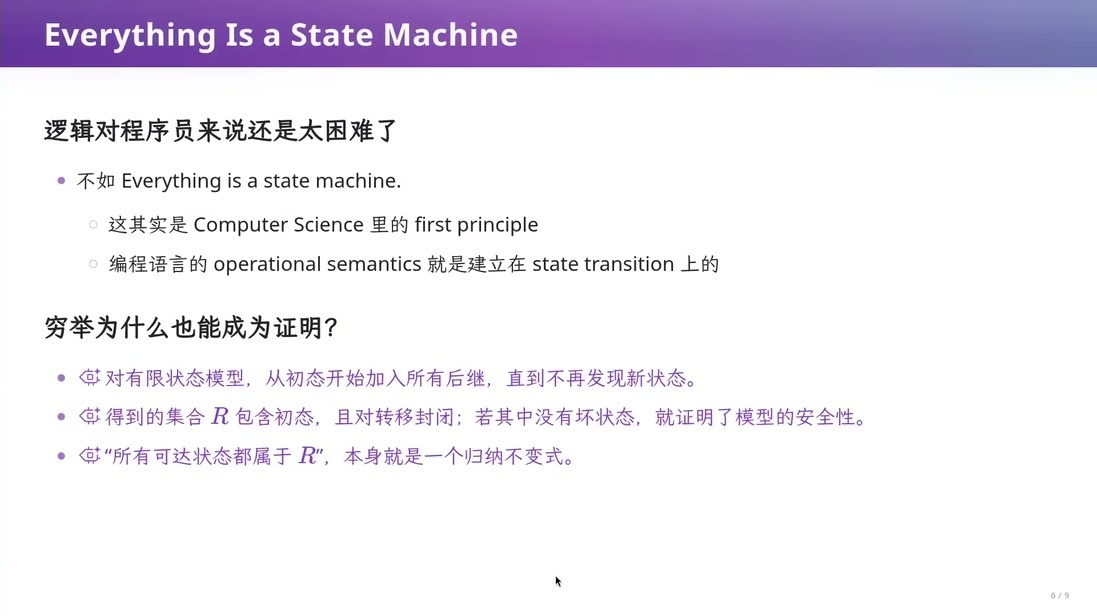
\includegraphics[width=0.88\textwidth]{figures/fig16_everything_is_state_machine.jpg}
\caption{Everything Is a State Machine：编程语言的操作语义建立在状态转移之上，完整穷举得到的可达闭包 $R^*$ 本身就是归纳不变式\vtag}
\label{fig:fig16_everything_is_state_machine}
\end{figure}
\srcnote{00:28:45--00:31:10}

我们可以把任何一个有限状态程序（或系统模型）形式化为一个状态迁移系统 $\mathcal{M} = (S, S_0, \to)$，其中 $S$ 是所有可能状态的集合（每个状态包含当前各变量的值、堆内存内容以及各线程的程序计数器 $\mathit{PC}$），$S_0 \subseteq S$ 是初始状态集合，$\to \;\subseteq S \times S$ 是单步执行转移关系。定义集合 $X \subseteq S$ 的单步后继算子 $\mathrm{Post}(X)$ 为：
\begin{equation}
\mathrm{Post}(X) \;\triangleq\; \{s' \in S \mid \exists s \in X:\; s \to s'\}
\label{eq:post_operator}
\end{equation}
从初始状态集 $S_0$ 出发，使用广度优先搜索（BFS）或深度优先搜索（DFS）不断将所有可能的后继状态加入集合，直到不再出现任何新状态为止，我们就得到了\textbf{可达状态集合（Reachable State Set）的不动点闭包 $R^*$}（对应配图）：
\begin{equation}
R_0 = S_0, \qquad R_{k+1} = R_k \cup \mathrm{Post}(R_k), \qquad R^* = \bigcup_{k=0}^{\infty} R_k \quad (\text{满足不动点 } R^* \cup \mathrm{Post}(R^*) = R^*)
\label{eq:reachable_closure_fixpoint}
\end{equation}

\begin{figure}[H]
\centering
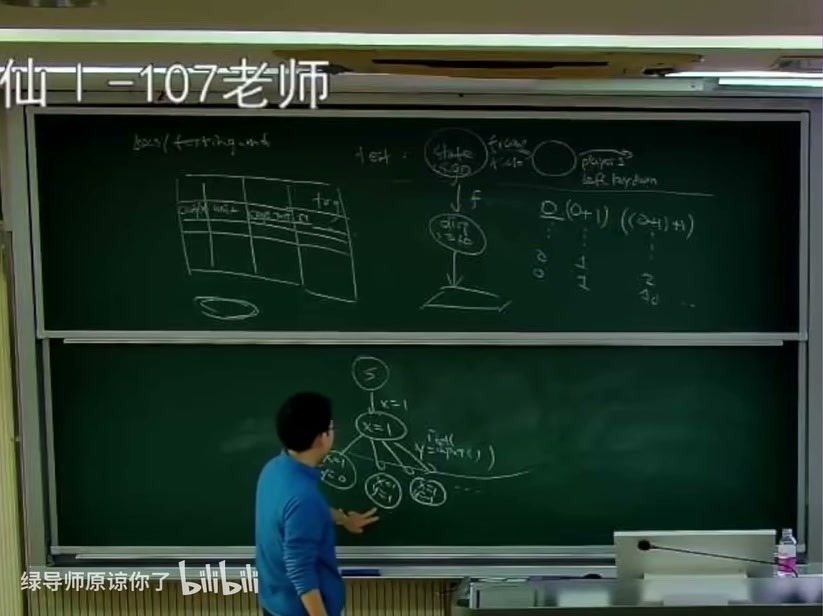
\includegraphics[width=0.72\textwidth]{figures/fig17_board_reachable_set_closure.jpg}
\caption{黑板板书：左侧展示外部输入 \texttt{y = input()} 引发的状态树分叉，右侧展示从初态逐层扩张直至转移封闭集合 $R^*$ 的穷举证明几何图景\vtag}
\label{fig:fig17_board_reachable_set_closure}
\end{figure}
\srcnote{00:29:10--00:31:05}

这里有一个极具启发性的理论问题：\textbf{为什么跑一万次随机测试不能算数学证明，而把有限状态模型穷举一遍就能算严格的数学证明？}
答案在于\textbf{转移封闭性（Closure under Transition）}！设不安全的坏状态（违反断言的状态）集合为 $B \subseteq S$。如果我们通过算法搜索构造出的状态集合 $R = R^*$ 同时满足以下三个条件：
\begin{equation}
\text{(1) 包含初态：} S_0 \subseteq R, \qquad
\text{(2) 转移封闭：} \mathrm{Post}(R) \subseteq R, \qquad
\text{(3) 不含坏状态：} R \cap B = \emptyset
\label{eq:model_checking_inductive_invariant}
\end{equation}
\begin{importantbox}{模型检查的第一性原理：转移封闭的可达集 $R^*$ 本身就是归纳不变式}
为什么跑一万次随机测试不能算证明，而模型检查器的暴力穷举却算严格的数学证明？因为当搜索到达不动点 $R^*$（满足 $S_0 \subseteq R^*$ 且 $\mathrm{Post}(R^*) \subseteq R^*$）时，“程序状态 $s$ 属于集合 $R^*$”这一性质天然满足初始化与单步保持两条归纳公理！只要验证 $R^* \cap B = \emptyset$，就从数学归纳法上彻底排除了到达任何坏状态 $B$ 的可能性。
\end{importantbox}

那么对照公式 \eqref{eq:loop_invariant_rules} 的归纳法三步曲就会恍然大悟：命题“当前状态 $s \in R$”在初始时刻成立（$S_0 \subseteq R$），每执行一步状态转移后依然成立（$\mathrm{Post}(R) \subseteq R$），且 $R$ 中没有任何坏状态（$R \cap B = \emptyset$）！换言之，\textbf{“所有可达状态都属于 $R^*$”这句看似废话的陈述，本身就是一个货真价实的数学归纳不变式！}这就是\textbf{模型检查（Model Checking）}的核心哲学：用机器的自动状态空间穷举，替代人类苦思冥想构造逻辑不变式的过程。

\subsection{Prove by Brute Force：并发计数器的状态交错模型检查}

为了展示“暴力穷举证明（Prove by Brute Force）”如何捕捉人类极易忽略的并发缺陷，我们来看上一讲出现过的双线程原子读写计数器 \texttt{T\_sum}（对应配图）：

\begin{figure}[H]
\centering
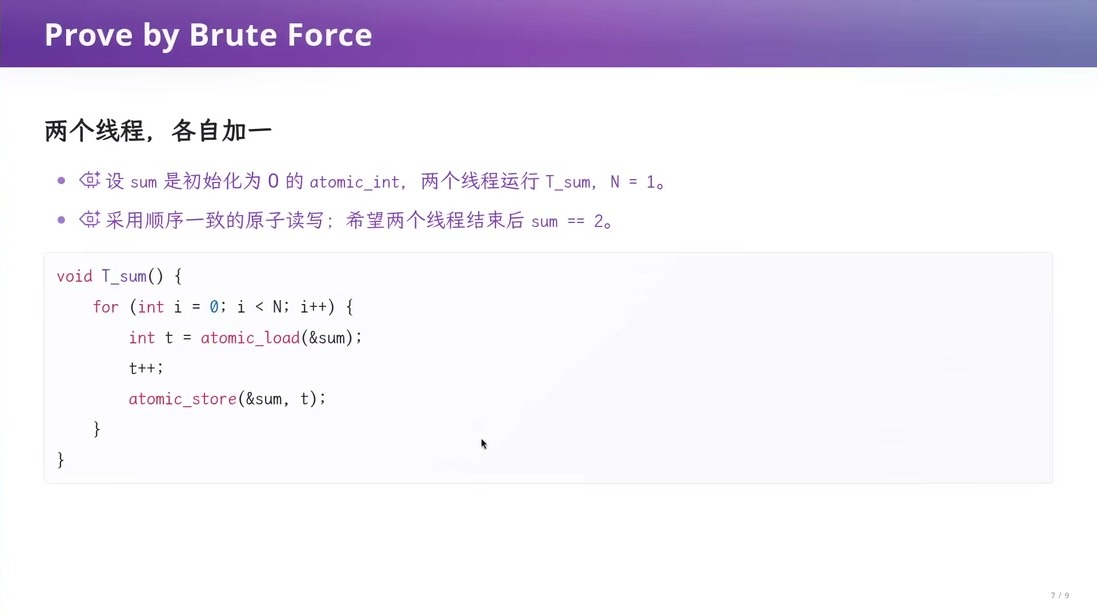
\includegraphics[width=0.88\textwidth]{figures/fig18_prove_by_brute_force_tsum.jpg}
\caption{Prove by Brute Force：两个线程各自执行一次 \texttt{T\_sum}（$N=1$），利用模型检查穷举顺序一致原子读写交错\vtag}
\label{fig:fig18_prove_by_brute_force_tsum}
\end{figure}
\srcnote{00:31:15--00:32:00}

\begin{lstlisting}[language=C, caption={双线程并发计数器模型（顺序一致原子读写，$N=1$）}]
void T_sum() {
    for (int i = 0; i < N; i++) {
        int t = atomic_load(&sum);  // L1: 读取共享原子变量 sum 到线程局部变量 t
        t++;                        // L2: 局部变量加一
        atomic_store(&sum, t);      // L3: 将 t 写回共享原子变量 sum
    }
}
\end{lstlisting}

假设全局变量 $\mathit{sum}$ 初值为 $0$，两个线程 $T_1, T_2$ 各自运行一次上述函数（$N = 1$），且 `\texttt{atomic\_load}` 与 `\texttt{atomic\_store}` 遵循顺序一致性（Sequential Consistency）语义。我们期望的后置条件是：当两个线程都结束时，$\mathit{sum} == 2$。

如果将每个全局状态表示为五元组 $s = (\mathit{sum},\; \mathit{pc}_1, t_1,\; \mathit{pc}_2, t_2)$，模型检查器只需从初态 $s_0 = (0,\; \mathrm{L1}, \bot,\; \mathrm{L1}, \bot)$ 出发穷举所有可能的线程交错，就会立刻找到一条通往错误终止状态 $\mathit{sum} = 1 \neq 2$ 的反例轨迹（Counterexample Trace）：
\begin{equation}
\begin{aligned}
s_0 = (0,\; \mathrm{L1}, \bot,\; \mathrm{L1}, \bot)
&\xrightarrow{T_1:\; \texttt{load}} (0,\; \mathrm{L2}, 0,\; \mathrm{L1}, \bot)
\xrightarrow{T_2:\; \texttt{load}} (0,\; \mathrm{L2}, 0,\; \mathrm{L2}, 0) \\
&\xrightarrow{T_1:\; \texttt{t++}} (0,\; \mathrm{L3}, 1,\; \mathrm{L2}, 0)
\xrightarrow{T_2:\; \texttt{t++}} (0,\; \mathrm{L3}, 1,\; \mathrm{L3}, 1) \\
&\xrightarrow{T_1:\; \texttt{store}} (1,\; \mathrm{Done}, 1,\; \mathrm{L3}, 1)
\xrightarrow{T_2:\; \texttt{store}} (1,\; \mathrm{Done}, 1,\; \mathrm{Done}, 1) \;\models\; (\mathit{sum} = 1 \neq 2)
\end{aligned}
\label{eq:tsum_counterexample_trace}
\end{equation}
更令人震惊的是，主讲教师在操作系统课上曾给出一个更强的定理：即便有任意多个线程、每个线程循环任意多次（$N \ge 2$），在非原子的读改写交错下，最终结束时依然存在一条调度轨迹使得 $\mathit{sum} = 2$！面对此类反直觉的并发调度，人类的直觉几乎必败无疑，而模型检查器却能毫不费力地给出精确到每一步指令的反例路径 \eqref{eq:tsum_counterexample_trace}。当我们把加一操作改为原子的读改写指令（如 `\texttt{atomic\_fetch\_add}`）或加互斥锁保护后，重新运行模型检查器，发现可达闭包 $R^*$ 中所有终止状态均满足 $\mathit{sum} == 2$，便完成了对该有限并发模型的严格证明。

\subsection{应对状态空间爆炸：从 BDD（$10^{20}$ 状态）到 BMC、CEGAR 与 IC3}

既然模型检查如此直接有效，为什么它没有一统江湖？因为它面临着一个与生俱来的宿敌——\textbf{状态空间爆炸（State Space Explosion）}。假设一个系统包含 $T$ 个并发组件（或线程），每个组件有 $L$ 个控制流位置，再加上取值域大小为 $D$ 的共享数据变量，那么组合状态空间的大小将随组件数量呈指数级增长：
\begin{equation}
|S| \;=\; \mathcal{O}\!\left(L^T \cdot D\right)
\label{eq:state_explosion_complexity}
\end{equation}
哪怕每个组件只有 $10$ 个状态，$20$ 个组件并行组合就会产生 $10^{20}$ 个状态——如果用哈希表逐个显式存储这些状态（Explicit-State Model Checking），全世界的内存加起来也远远不够。

因此，自 1981--1982 年 Clarke--Emerson 与 Queille--Sifakis 独立创立模型检查（后获 2007 年图灵奖）以来，该领域四十余年的演进史，本质上就是一部\textbf{“改变状态表示方法与搜索策略”}的突围史（对应配图 与对应配图）：

\begin{figure}[H]
\centering
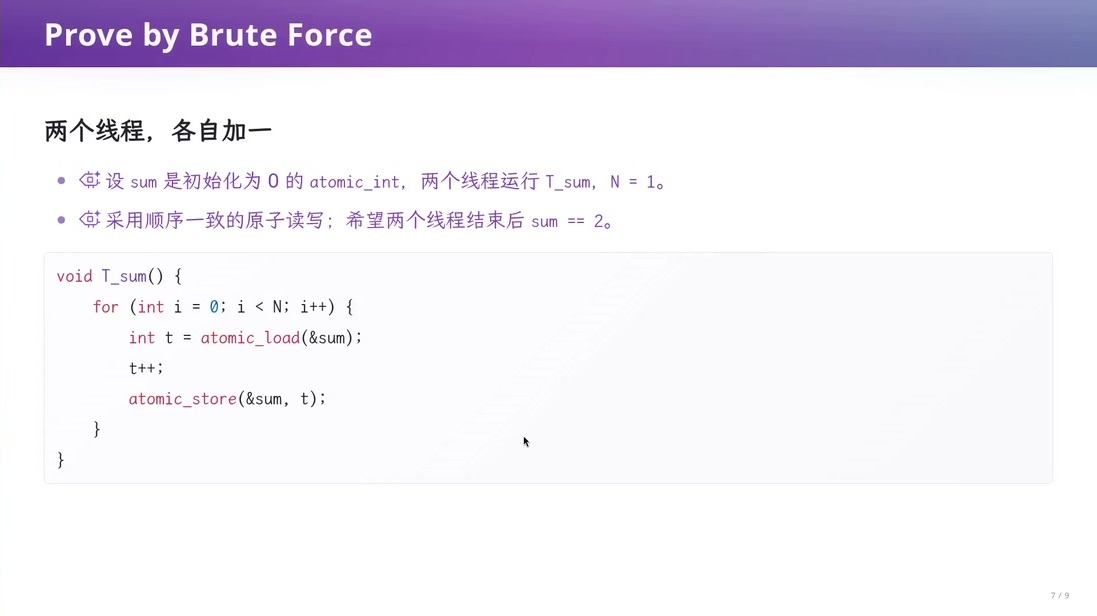
\includegraphics[width=0.88\textwidth]{figures/fig19_symbolic_model_checking_bdd.jpg}
\caption{状态爆炸与改变表示方法：1981--1982 年模型检查诞生，以及 1990年 Burch 等人提出符号模型检查（Symbolic Model Checking）突破 $10^{20}$ 状态\vtag}
\label{fig:fig19_symbolic_model_checking_bdd}
\end{figure}
\srcnote{00:32:05--00:32:40}

\begin{enumerate}
    \item \textbf{1990年：符号模型检查（Symbolic Model Checking）与二叉决策图（BDD）}：Burch、Clarke、McMillan、Dill 与 Hwang 在 \textbf{1990年}发表了里程碑论文《Symbolic Model Checking: $10^{20}$ States and Beyond》。他们的核心洞见是：\textbf{不要逐个枚举状态，而是用布尔公式的特征函数 $\chi_X(\vec{v})$ 表示一整组状态集合 $X$，并用有序二叉决策图（OBDD）对状态集合和转移关系 $\chi_T(\vec{v}, \vec{v}')$ 直接做集合代数运算！}当系统结构具有规律性时，包含 $10^{20}$ 个状态的集合可能只需几百个节点的 BDD 就能紧凑表示。当然，这种压缩高度依赖问题结构，一旦遇到乘法器等对 BDD 不友好的电路，BDD 本身也会发生节点爆炸。
    \item \textbf{1999年：有界模型检查（Bounded Model Checking，BMC）与 SAT 求解器}：既然求无穷步不动点 $R^*$ 太贵，Biere 等人在 1999 年提出退一步问一个有界问题：\textbf{“是否存在一条长度不超过 $k$ 步的错误执行轨迹？”}该问题可以直接展开编码为一个命题逻辑可满足性（SAT）公式：
    \begin{equation}
    \mathrm{BMC}_k(\mathcal{M}, P) \;\triangleq\; I(s_0) \;\land\; \bigwedge_{i=0}^{k-1} T(s_i, s_{i+1}) \;\land\; \left(\bigvee_{i=0}^{k} \neg P(s_i)\right)
    \label{eq:bmc_sat_encoding}
    \end{equation}
    将公式 \eqref{eq:bmc_sat_encoding} 交给现代 CDCL SAT 求解器：如果可满足（SAT），求解器给出的变量赋值就是一条长度为 $\le k$ 的具体反例轨迹；如果不可满足（UNSAT），则证明了系统在前 $k$ 步内绝对安全（但尚未直接推广到任意步数 $k \to \infty$）。
    \item \textbf{2000 年（CEGAR）与 2011 年（IC3 / PDR）：让反例指导发现不变式}：如对应配图 所示，Clarke 等人在 2000 年提出\textbf{反例引导的抽象精化（CEGAR）}——先在忽略细节的粗糙抽象模型上做检查，若发现反例，再去真实系统中检验该反例是否真的可行；若是假反例（Spurious Counterexample），则只把排除该假反例所需的最小细节补回抽象模型。到了 2011 年，Aaron R. Bradley 提出了震惊验证界的 \textbf{IC3（Incremental Construction of Inductive Clauses for Indubitable Correctness，又称 PDR）}算法：维护一列逐帧逼近的过近似状态集公式 $F_0, F_1, \dots, F_k$，满足：
    \begin{equation}
    F_0 = I, \qquad F_i \implies F_{i+1}, \qquad F_i \implies P, \qquad F_i \land T \implies F_{i+1}'
    \label{eq:ic3_pdr_frames}
    \end{equation}
    一旦在某一步出现相邻两帧等价（$F_i \equiv F_{i+1}$），该 $F_i$ 就自动收敛为一个完备的\textbf{归纳不变式（Inductive Invariant）}！这意味着，过去必须靠程序员绞尽脑汁想出来的循环不变式 $I$，如今也能作为算法在反例阻断（Cube Blocking）过程中自动搜索合成的产物。
\end{enumerate}

\begin{figure}[H]
\centering
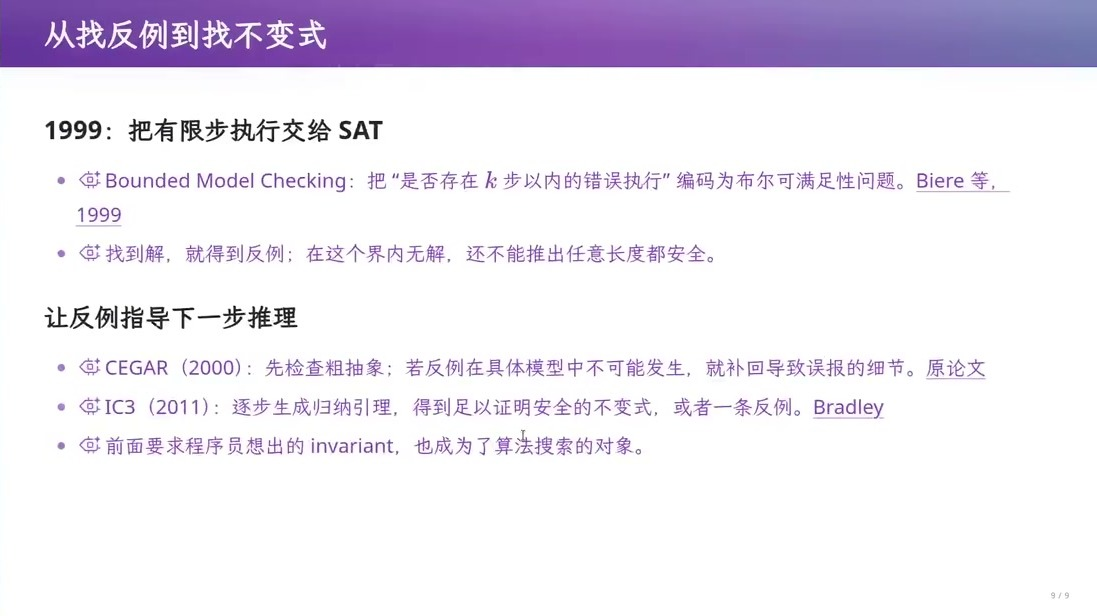
\includegraphics[width=0.88\textwidth]{figures/fig20_bmc_cegar_ic3_slide.jpg}
\caption{从找反例到找不变式：1999 年有界模型检查（BMC）交给 SAT，以及 CEGAR（2000）与 IC3（2011）利用反例自动生成归纳引理\vtag}
\label{fig:fig20_bmc_cegar_ic3_slide}
\end{figure}
\srcnote{00:32:42--00:32:50}

\begin{knowledgebox}{模型检查四十年突围路线：从显式枚举、BDD、BMC 到 IC3/PDR}
面对组合状态数按 $|S| = \mathcal{O}(L^T \cdot D)$ 指数增长的状态爆炸难题，模型检查领域演化出了三代核心武器：（1）\textbf{符号模型检查（1990）}用布尔公式与二叉决策图（BDD）紧凑表示状态集合，一举突破 $10^{20}$ 状态；（2）\textbf{有界模型检查 BMC（1999）}将“$k$ 步内是否出错”编码为 SAT 问题快速寻找反例；（3）\textbf{CEGAR（2000）与 IC3/PDR（2011）}利用反例阻断逐帧构造相对归纳子句，让算法自动搜索合成过去必须靠人类专家手写的归纳不变式。
\end{knowledgebox}

在切换章节时，视频画面还短暂闪过了主讲教师编写本讲幻灯片的 Vim 编辑器源码 \texttt{p12/lect/index.md}（对应配图）：可以看到主讲教师在 Markdown 讲义大纲中使用诸如 \texttt{[[介绍一下model checking领域的一些主要进展，以及在今天回看的意义]]}、\texttt{[[配一个真实的TLA+模型和检验案例示意图]]}、\texttt{[[画一个路径搜索图，强调合并等价类]]} 等双括号结构化元指令，驱动 AI 辅助补全文献链接与可视化图表——这本身正是本课程所倡导的“人把握核心脉络与品味、Agent 承担繁琐工程实现”的生动写照。

\begin{figure}[H]
\centering
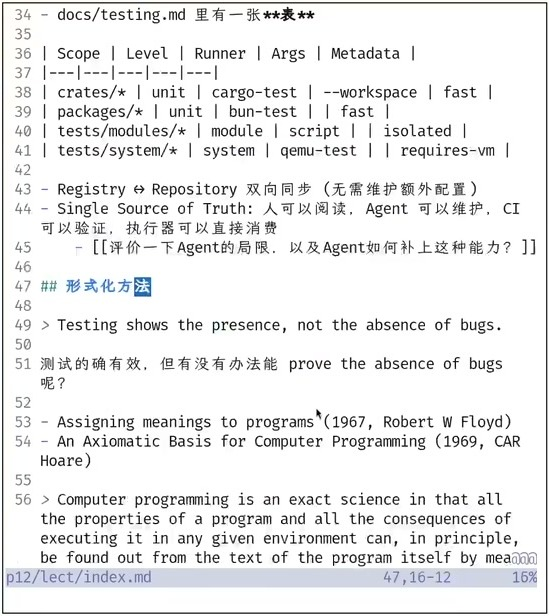
\includegraphics[width=0.78\textwidth]{figures/fig21_vim_slide_prompt_source.jpg}
\caption{讲义源码一瞥：主讲教师在 \texttt{p12/lect/index.md} 中用双括号指令组织模型检查、TLA+ 与 KLEE 案例的生成式备课工作流\vtag}
\label{fig:fig21_vim_slide_prompt_source}
\end{figure}
\srcnote{00:32:50--00:32:55}

% =========================================================================
% SECTION 5
% =========================================================================
\section{模型、路径与完整证明：TLA+、KLEE、CompCert 与 seL4}

尽管真实软件系统的规模远超玩具程序，但人类从未放弃将形式化证明带入工业级软件的努力，而是分化出了三条极具代表性的技术路线：\textbf{基于抽象模型的验证（Model-Based：TLA+）}、\textbf{基于符号路径的验证（Path-Based：KLEE）}以及\textbf{基于完整定理证明的基础软件验证（Proof-Based：CompCert 与 seL4）}。

\subsection{Model-Based（TLA+）：从自动售货机、两阶段提交（2PC）到精化映射}

当一个真实软件有几万乃至几十万行代码时，直接对源码做状态空间穷举是不现实的。但正如模型检查领域在 \textbf{1980年}代经常探讨的经典\textbf{自动售货机（Vending Machine）}案例那样：一台真实的自动售货机内部包含驱动摄像头、识别纸币花纹、给硬币称重防伪、控制步进电机掉货等上万行繁琐的底层 C 代码；但如果我们关心的是“投币、选货与退币的账目逻辑会不会出错或卡死”，我们完全可以把底层硬件细节抽象掉，建立一个只包含“当前余额状态（$0$ 元、$1$ 元、$5$ 元、$6$ 元……）”与“投币/退币/出货转移边”的几十个状态的有限状态机模型，先在这个核心模型上用暴力搜索完成严格证明！

Leslie Lamport 创立的 \textbf{TLA+（Temporal Logic of Actions）}正是这一思想在分布式系统领域的集大成者（对应配图）。以分布式数据库中经典的\textbf{两阶段提交（Two-Phase Commit，2PC）}协议为例（源自 Gray \& Lamport《Consensus on Transaction Commit》附录 A.2）：
\begin{itemize}
    \item \textbf{高层抽象规范（\texttt{TCommit}）}：只声明整个分布式事务不可违背的核心一致性安全属性（Safety Property）——在任何时刻，绝不允许出现一个资源管理器（RM）已经提交（\texttt{committed}）、而另一个资源管理器却已经中止（\texttt{aborted}）的矛盾状态：
    \begin{equation}
    \mathsf{TCSpec\_Safety} \;\triangleq\; \Box\,\neg\Big(\exists i, j \in \mathrm{RM}:\; \mathit{rmState}[i] = \mathsf{committed} \;\land\; \mathit{rmState}[j] = \mathsf{aborted}\Big)
    \label{eq:2pc_safety_spec}
    \end{equation}
    \item \textbf{具体协议模型（\texttt{TwoPhase.tla}）}：引入事务协调者（TM）与各个参与者（RM）之间的消息收发状态（\texttt{Working} $\to$ \texttt{Prepared} $\to$ \texttt{Committed / Aborted}）。在论文的 TLC 模型检查实验中，针对 $6$ 个参与者（RM），TLC 穷举了全部 $50,816$ 个可达状态，自动验证了类型不变式与精化性质 \texttt{TPSpec $\Rightarrow$ TC!TCSpec} 成立。
\end{itemize}

\begin{figure}[H]
\centering
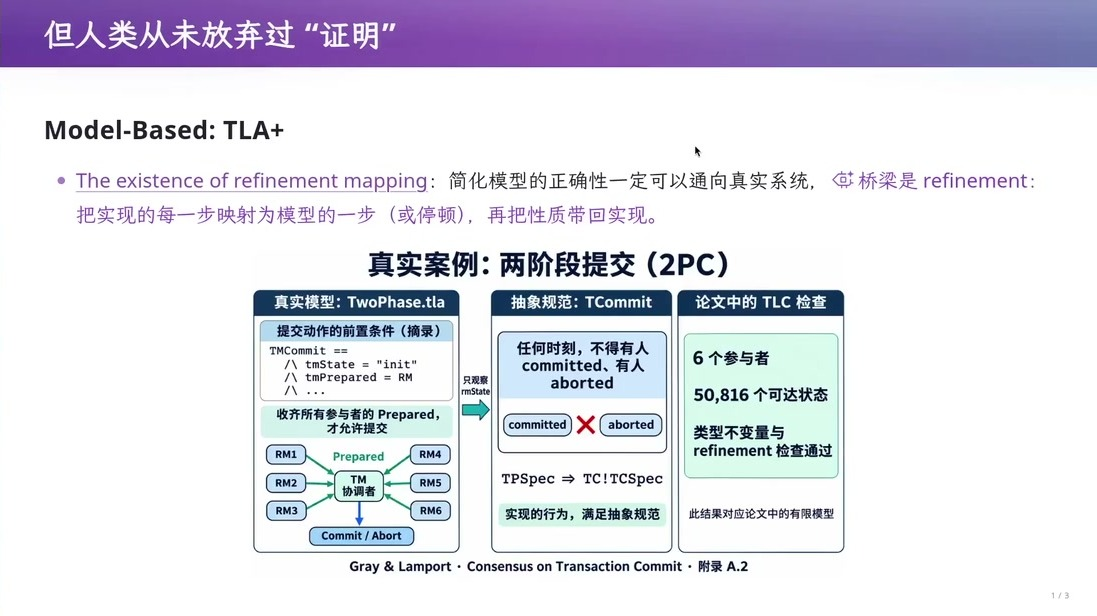
\includegraphics[width=0.88\textwidth]{figures/fig22_tlaplus_2pc_refinement.jpg}
\caption{Model-Based（TLA+）：精化映射（Refinement Mapping）与两阶段提交（2PC，6 个参与者、50,816 个可达状态）真实检验案例\vtag}
\label{fig:fig22_tlaplus_2pc_refinement}
\end{figure}
\srcnote{00:32:55--00:37:50}

然而，这里有一个必须严肃回答的工程追问：\textbf{“简化模型被证明百分之百正确，凭什么能说明我写的真实 C/Rust 代码也是正确的？”}如果代码第一行就直接写个 `\texttt{return 0;}`，或者像主讲教师分享的生活趣事那样——在自动售货机买饮料时货没掉下来触发了自动退款，紧接着再买一瓶时前面卡住的那瓶连同新买的一起掉了两瓶下来（因为真实代码里有红外掉货传感器重试逻辑，而抽象模型里压根没建模“卡货掉双份”这一物理状态）——模型正确性岂不成了空中楼阁？

连接高层抽象模型 $\mathcal{M}_A = (S_A, S_{0,A}, \to_A)$ 与底层具体系统 $\mathcal{M}_C = (S_C, S_{0,C}, \to_C)$ 的数学桥梁，就是 Martín Abadi 与 Leslie Lamport 在经典论文《The Existence of Refinement Mappings》中严格阐述的\textbf{精化映射（Refinement Mapping）}（对应配图）：

\begin{figure}[H]
\centering
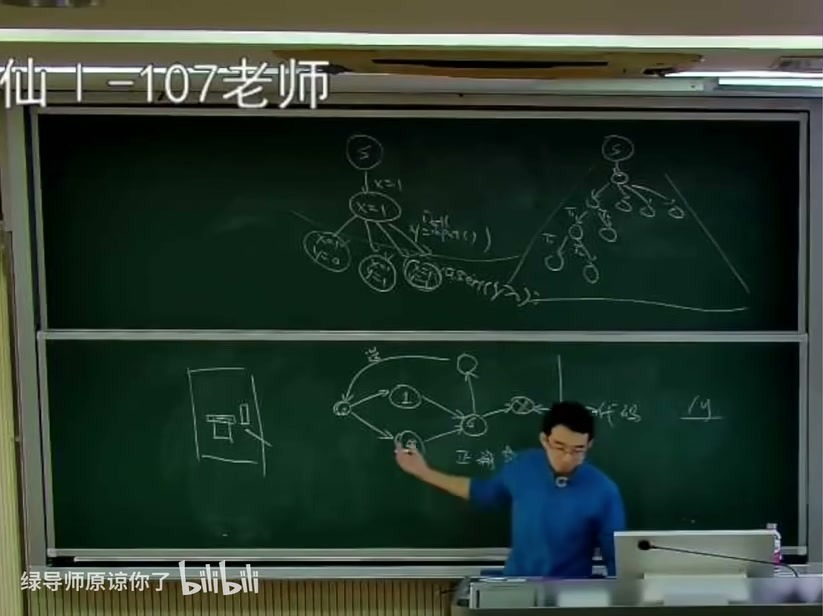
\includegraphics[width=0.72\textwidth]{figures/fig23_board_refinement_mapping.jpg}
\caption{黑板板书：具体状态机步进向抽象状态机步进（或停顿步 Stuttering Step）投射的精化映射（Refinement Mapping）交换图\vtag}
\label{fig:fig23_board_refinement_mapping}
\end{figure}
\srcnote{00:37:55--00:42:20}

定义一个从具体状态空间到抽象状态空间的投射函数（状态抽象函数）$\alpha: S_C \to S_A$。如果 $\alpha$ 满足以下两个条件：
\begin{equation}
\begin{cases}
\textbf{1. 初态保持：} & \forall s_0 \in S_{0,C}:\; \alpha(s_0) \in S_{0,A} \\[4pt]
\textbf{2. 步进模拟（含停顿步 Stuttering）：} & \forall (s, s') \in \to_C:\; \big(\alpha(s), \alpha(s')\big) \in \to_A \;\lor\; \alpha(s) = \alpha(s')
\end{cases}
\label{eq:refinement_mapping_condition}
\end{equation}
那么具体系统 $\mathcal{M}_C$ 的每一条执行轨迹 $s_0 \to_C s_1 \to_C s_2 \to_C \cdots$，在经过 $\alpha$ 投射并合并相邻重复状态（即具体层修改了缓冲区或局部变量、但在抽象层看来状态未变的\textbf{停顿步 Stuttering Step}，好比机械表分针走了 59 格而小时数保持不变）之后，都必然对应抽象模型 $\mathcal{M}_A$ 中一条合法的轨迹！由此，在抽象模型 $\mathcal{M}_A$ 上证明的一切安全性定理（如公式 \eqref{eq:2pc_safety_spec}），都会通过精化映射 $\alpha$ 自动继承到具体系统 $\mathcal{M}_C$ 上。

在课堂演示至 39 分钟处，由于教室麦克风出现轻微爆音，主讲教师还顺手切出终端界面，展示了本地 AI Agent 自动执行 `\texttt{dmesg}` 与 `\texttt{journalctl -b -p warning}` 排查内核与 PipeWire 音频设备状态日志的实时过程（对应配图）。\begin{practicebox}{工程落地技巧：用 TLA+ 精化映射指导真实代码的日志轨迹对齐测试}
在工业界开发分布式共识或事务协议（如 Two-Phase Commit 或 Raft）时，即便没有资源像 seL4 那样完成从模型到源码的形式化精化证明，也可以通过\textbf{轨迹对齐测试（Trace Conformance Testing）}架起桥梁：在真实系统每次发生关键状态跃迁时打印结构化日志 $\alpha(s_k)$，同时用 TLA+ 模型生成海量极端交错测试用例，验证真实系统打印的状态转移序列是否为 TLA+ 允许轨迹的合法精化投影。
\end{practicebox}

而在工程实践中，即便我们没有足够的人力去手写从 TLA+ 到 C 代码的完整形式化精化证明，我们依然可以利用精化映射 $\alpha$ 的思想做\textbf{模型引导的轨迹对齐测试（Model-Guided Trace Conformance Checking）}：在 TLA+ 模型上采样生成海量边缘状态转移序列，同时在真实代码关键节点打印状态日志 $\alpha(s_k)$，自动比对代码运行日志与 TLA+ 模型轨迹是否完全吻合！

\begin{figure}[H]
\centering
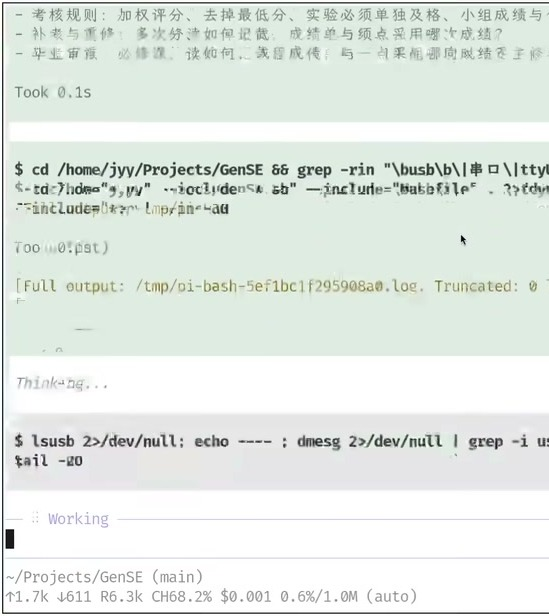
\includegraphics[width=0.78\textwidth]{figures/fig24_terminal_agent_dmesg_diagnosis.jpg}
\caption{终端实战插曲：AI Agent 自动调用 \texttt{dmesg} 与 \texttt{journalctl} 检查内核驱动与音频子系统状态日志\vtag}
\label{fig:fig24_terminal_agent_dmesg_diagnosis}
\end{figure}
\srcnote{00:39:05--00:39:25}

\subsection{Path-Based（KLEE）：用符号执行与路径约束求解合并等价类}

如果不想额外写一份 TLA+ 模型，能不能直接在真实的 C 程序代码上做穷举证明？这就是以 \textbf{KLEE}（Cadar, Dunbar \& Engler, OSDI 2008）为代表的\textbf{符号执行（Symbolic Execution）}路线（对应配图）。

\begin{figure}[H]
\centering
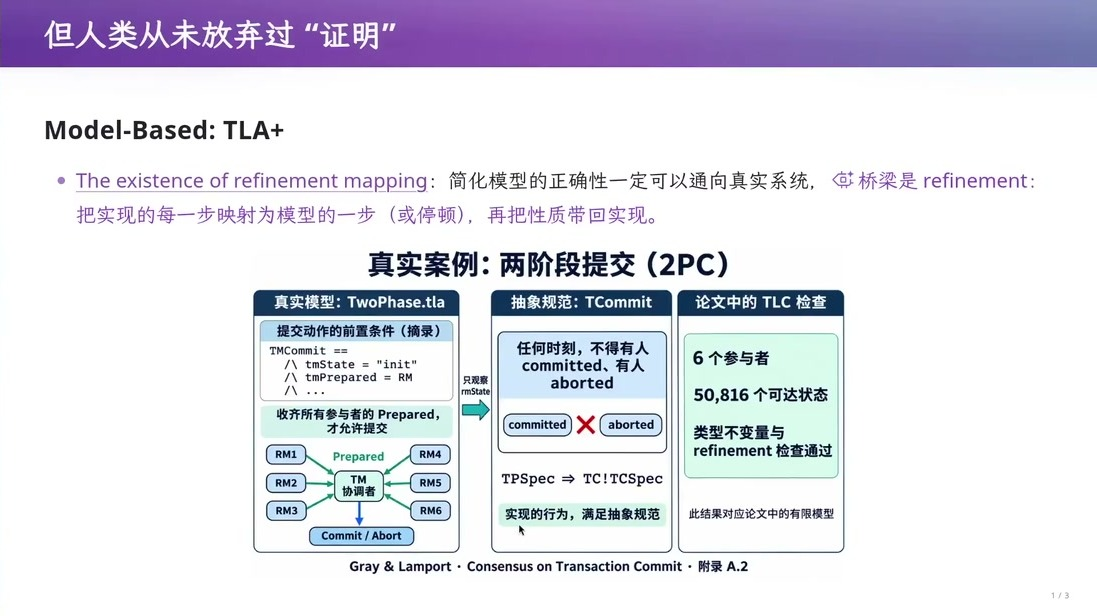
\includegraphics[width=0.88\textwidth]{figures/fig25_klee_symbolic_execution.jpg}
\caption{Path-Based（KLEE）：将 32 位有符号整数 $x$ 的 $2^{32}$ 个具体输入按分支路径约束 $\mathit{PC}$ 合并为 3 个等价类（$x=0$、$x<0$、$x>0$）\vtag}
\label{fig:fig25_klee_symbolic_execution}
\end{figure}
\srcnote{00:42:30--00:47:25}

考虑对应配图 中的符号函数 `\texttt{get\_sign(int x)}`：
\begin{lstlisting}[language=C, caption={KLEE 符号执行入门示例 \texttt{get\_sign}}]
int get_sign(int x) {
    if (x == 0) return 0;
    if (x < 0)  return -1;
    return 1;
}
\end{lstlisting}
如果用黑盒暴力枚举来测这个 32 位有符号整数函数，输入空间大小高达 $|\mathcal{X}| = 2^{32} \approx 4.29 \times 10^9$。但为什么我们要傻乎乎地把 $-1, -2, -3, \dots$ 挨个跑一遍？它们在程序里走的分明是完全同一条执行路径！

符号执行的绝妙之处在于：\textbf{不给输入变量赋具体数值，而是将其设为一个代数符号 $x = \alpha$，把程序的每一步执行转化为维护“符号状态映射 $\sigma$”与“路径约束（Path Condition，$\mathit{PC}$）”的代数方程组}。例如在主讲教师黑板推导的例子中，若初态令 $x = 1$，读入符号输入 $y = \beta$，执行 `\texttt{z = x + y}` 后符号状态为 $\sigma = \{x \mapsto 1,\; y \mapsto \beta,\; z \mapsto 1 + \beta\}$；当遇到条件分支 `\texttt{if (B)}` 时，符号执行器将搜索树一分为二，分别把分支条件及其否定追加到路径约束中：
\begin{equation}
\mathit{PC}_{\text{taken}} = \mathit{PC} \;\land\; \sigma(B), \qquad
\mathit{PC}_{\text{not-taken}} = \mathit{PC} \;\land\; \neg \sigma(B)
\label{eq:symbolic_execution_branch}
\end{equation}
对于 `\texttt{get\_sign(int x)}`，整棵符号执行树只有 $3$ 条叶子路径，完美地将 $2^{32}$ 个输入划分为 $3$ 个互不相交的等价类：
\begin{equation}
\Pi_1:\; \mathit{PC}_1 \equiv (x = 0), \qquad
\Pi_2:\; \mathit{PC}_2 \equiv (x \neq 0 \land x < 0), \qquad
\Pi_3:\; \mathit{PC}_3 \equiv (x \neq 0 \land x \ge 0)
\label{eq:klee_three_partitions}
\end{equation}
在任意一条路径 $\Pi_i$ 上，如果我们想验证断言性质 $P$（例如指针非空、数组不越界或除数非零 $y \neq 0$）是否恒成立，只需向底层 SMT 自动定理求解器（如 Z3 或 STP）发起如下可满足性查询：
\begin{equation}
\mathrm{Query}(\Pi_i, P) \;\triangleq\; \mathrm{SAT}\!\big(\mathit{PC}_i \;\land\; \neg \sigma_i(P)\big)
\label{eq:klee_smt_query}
\end{equation}
\begin{itemize}
    \item 若公式 \eqref{eq:klee_smt_query} 返回 \textbf{SAT（可满足）}：求解器解出的一组具体变量赋值 $\alpha^*$ 就是一个百分百能触发该路径下断言失败的\textbf{高价值具体测试用例}！
    \item 若公式 \eqref{eq:klee_smt_query} 返回 \textbf{UNSAT（不可满足）}：则在精确的指令集语义（KLEE 基于 LLVM IR 位精确语义）下，\textbf{证明了落入该等价类路径的所有输入都绝对不会违反性质 $P$}！
\end{itemize}

\begin{knowledgebox}{符号执行（Symbolic Execution）的核心权衡：等价类合并 vs. 路径爆炸}
KLEE 等符号执行引擎通过将具体输入替换为符号变量 $\alpha$ 并收集分支路径约束 $\mathit{PC}_i$，把原本高达 $2^{32}$ 的输入空间压缩为按执行路径划分的有限等价类，再交由 SMT 求解器判定 $\mathrm{SAT}(\mathit{PC}_i \land \neg P)$。但符号执行同样面临两大工程挑战：一是需要对底层指令集（如 LLVM IR 或 WASM）的全部运算建立位精确方程模型；二是当遇到含外部输入的循环或复杂系统调用时，路径数量依然会呈指数级分叉。
\end{knowledgebox}

\subsection{Proof-Based（CompCert 与 seL4）：人类基础软件形式化验证的双子巅峰}

如果连模型抽象（TLA+）和路径限界（KLEE）的折中都不接受，能不能从头到尾在公理系统里严格证明一个工业级大型基础软件的源代码符合规格？这听起来像是天方夜谭，但在计算机科学史上，真有两支团队做成了这件“疯狂的事情”，并因此永载史册（对应配图）：

\begin{figure}[H]
\centering
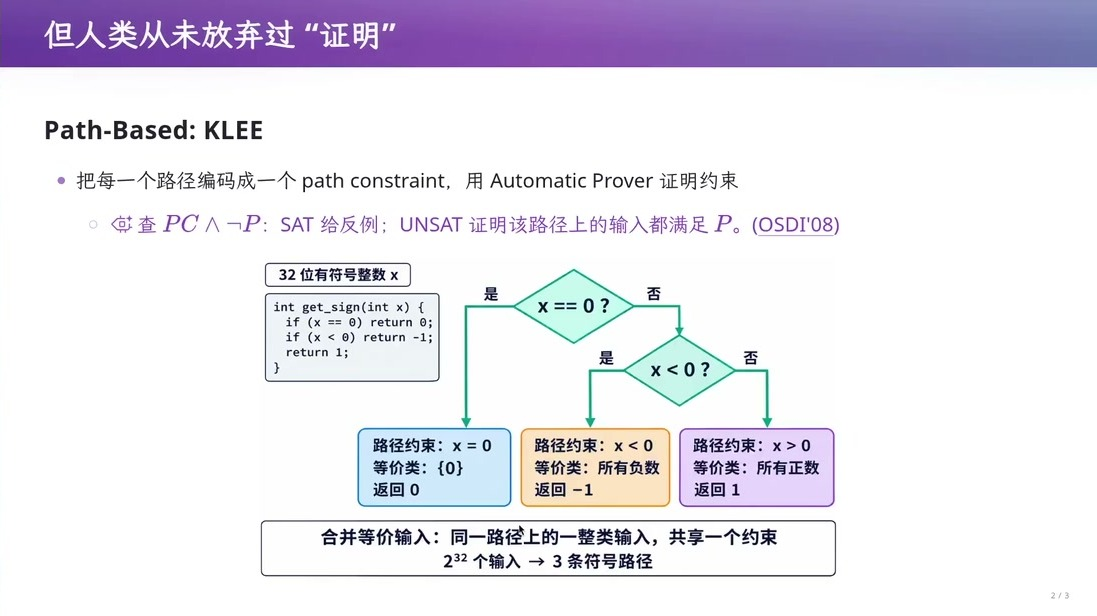
\includegraphics[width=0.88\textwidth]{figures/fig26_compcert_and_sel4.jpg}
\caption{Proof-Based（CompCert 和 seL4）：证明编译器保持程序语义的 CompCert（3 人年、4.2万行 Coq）与证明内核 C 实现符合抽象规范的 seL4（25人年、20万行证明脚本）\vtag}
\label{fig:fig26_compcert_and_sel4}
\end{figure}
\srcnote{00:47:30--00:51:10}

\begin{enumerate}
    \item \textbf{CompCert：经过形式化验证的 C 语言编译器（Xavier Leroy 等）}：
    普段程序员总是盲目信任编译器（Blind Trust），觉得只要自己写的 C 代码逻辑正确，\texttt{gcc} 或 \texttt{clang} 编译出的机器码就一定正确。但实际上，现代优化编译器自身也是几十万行的复杂软件，完全可能存在编译 Bug——要么在编译合法程序时直接崩溃，要么在激进优化时发生错误翻译（Miscompilation，例如把原本应该返回 $1$ 的函数错误生成了把 $2$ 写入返回寄存器的汇编指令）！
    为了彻底消除编译器误编译风险，Xavier Leroy 团队从 \textbf{06年}、\textbf{07年}前后的早期版本起步，在 \textbf{2009年}（即 \textbf{09年}）发表的 CACM 经典论文《Formal Verification of a Realistic Compiler》中，使用 Coq 证明助手完整证明了从 C 语言子集（Clight）经过十余趟中间表示（RTL、LTL、Linear、Mach）直到 PowerPC/ARM/x86 汇编代码的\textbf{语义保持定理（Semantic Preservation Theorem）}：
    \begin{equation}
    \forall S, C:\; \big(\mathrm{Compile}(S) = \mathrm{OK}(C) \;\land\; \mathrm{Safe}(S)\big) \implies \forall B \in \mathrm{Behaviors}(C),\; B \in \mathrm{Behaviors}(S)
    \label{eq:compcert_semantic_preservation}
    \end{equation}
    公式 \eqref{eq:compcert_semantic_preservation} 保证了：只要源程序 $S$ 不触发未定义行为且编译成功生成目标码 $C$，那么目标码 $C$ 在硬件上运行产生的任何可观测行为轨迹 $B$，都必定是源程序 $S$ 语义所允许的合法行为！根据 \textbf{2009年}论文统计，CompCert 的形式化与证明耗费了约 \textbf{3 人年}，共计 \textbf{4.2万}行 Coq 代码，其中高达 \textbf{76\%} 的代码量是纯粹的数学证明脚本。
    \item \textbf{seL4：经过完整形式化验证的操作系统微内核（Gerwin Klein 等，SOSP 2009）}：
    同样在 \textbf{2009年}，NICTA（澳大利亚国家信息通信技术研究院）团队在 Isabelle/HOL 证明助手中完成了对 \textbf{seL4} 微内核从高层抽象规范（Abstract Specification）到可执行设计规范（Executable Spec）再到最终 C 语言实现的端到端精化证明，严格保证了内核在满足前置假设下绝不会发生空指针解引用、缓冲区溢出、死循环或未授权信息泄露。首次完成时，整个项目从设计、实现到形式化验证累计投入约 \textbf{25人}年（25 person-years），撰写了约 \textbf{20万}行 Isabelle 证明脚本！
\end{enumerate}

\begin{importantbox}{为什么值得为编译器和操作系统内核付出如此高昂的证明代价？}
正如主讲教师所言，如果一段代码是要装在登月探测器或心脏起搏器上的，哪怕上层应用代码已经用形式化方法证明得滴水不漏，只要底层的编译器翻错了一条指令、或者底层的操作系统内核在中断切换时踩坏了一个寄存器，上层所有的正确性保证就会瞬间灰飞烟灭！\textbf{编译器与操作系统内核是整个软件生态共同依赖的底座（Trusted Computing Base，TCB）}：虽然花费 3 人年（4.2万行 Coq）或 25人年（20万行证明）看似极其昂贵，但这份投入会在未来成千上万次编译和每一次系统调用中反复产生复利回报。
\end{importantbox}

% =========================================================================
% SECTION 6
% =========================================================================
\section{证明助手（Proof Assistant）：铁面无私的反馈工作台}

\subsection{OpenAI“数学核弹”背后的基础设施：为什么中学数学草稿纸不够严格？}

既然 CompCert 和 seL4 证明了“用计算机严格验证大型软件”在理论上完全可行，唯一的瓶颈是昂贵的人类专家工时（3 人年、25人年），那么当大语言模型（LLM）出现后，为什么形式化数学与软件验证突然迎来了爆发式突破（课堂上戏称为 OpenAI 丢下的“数学核弹”）？

答案就在于所有现代形式化定理证明共同依赖的底座——\textbf{证明助手（Proof Assistant，如 Lean 4、Coq / Rocq、Isabelle/HOL）}（对应配图）。

\begin{figure}[H]
\centering
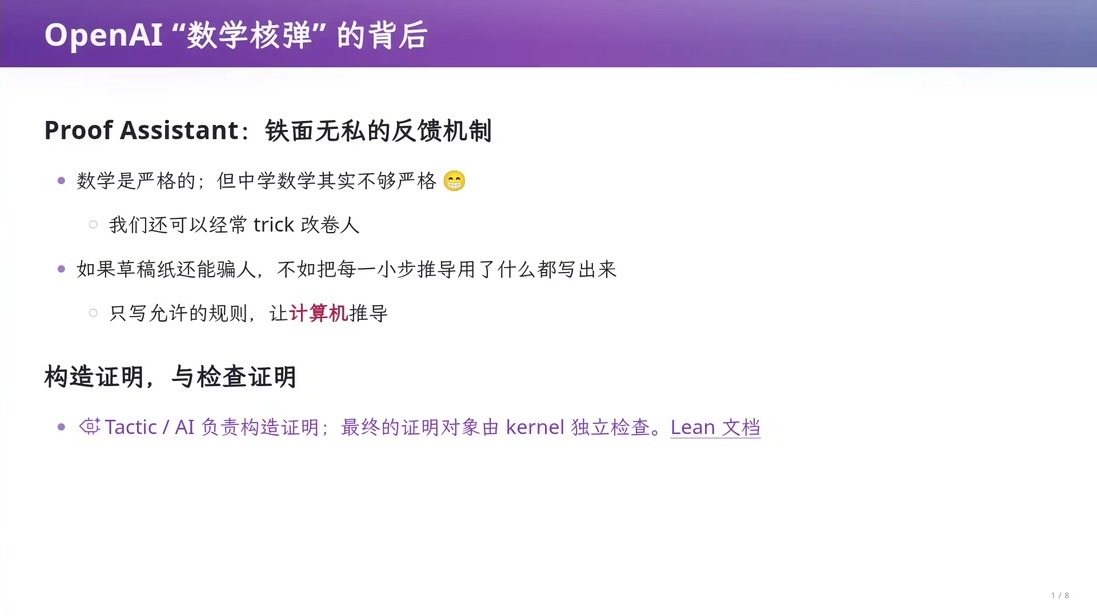
\includegraphics[width=0.88\textwidth]{figures/fig27_proof_assistant_feedback.jpg}
\caption{OpenAI“数学核弹”的背后：Proof Assistant 铁面无私的反馈机制——Tactic 与 AI 负责构造证明，最终证明对象由极简 Kernel 独立检查\vtag}
\label{fig:fig27_proof_assistant_feedback}
\end{figure}
\srcnote{00:51:15--00:53:40}

回想我们在中学或大学离散数学考试中写数学证明的过程：人类的自然语言数学证明其实充满了跳跃与“善意的糊弄”。算不出解析解时可以先猜一个答案，中间卡壳的步骤写一句“同理可得”“显然成立（Obviously）”，甚至草稿纸上前面算错了一个负号、后面又算错一个负号“负负得正”蒙对了最终结果，阅卷老师改卷改得疲惫时往往也就大笔一挥给过了。如果让大模型直接用自然语言写数学证明，它同样极其擅长用华丽流畅的数学黑话把关键漏洞糊弄过去。

而 Proof Assistant 彻底终结了任何“糊弄”的可能：它把草稿纸变成了一个\textbf{只认公理规则、逐字符严格匹配的确定性状态机工作台}（对应配图）。

\begin{figure}[H]
\centering
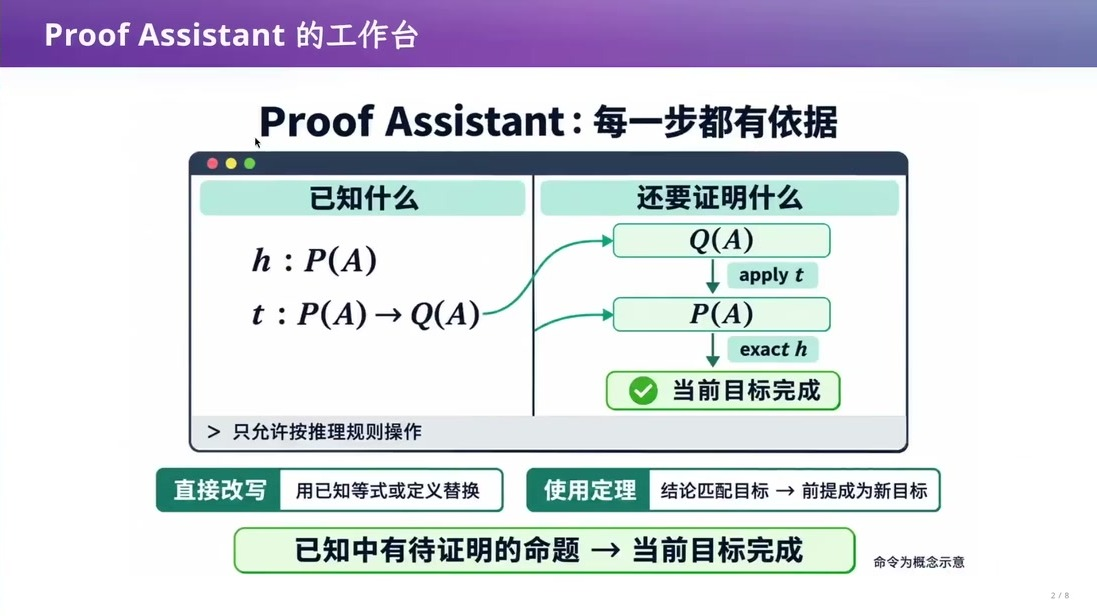
\includegraphics[width=0.88\textwidth]{figures/fig28_proof_assistant_workbench.jpg}
\caption{Proof Assistant 的工作台：左侧列出已知假设上下文，右侧列出待证明目标，每一步只能通过合法推理规则（如 \texttt{apply t}、\texttt{exact h}）改变证明状态\vtag}
\label{fig:fig28_proof_assistant_workbench}
\end{figure}
\srcnote{00:53:45--00:54:30}

如对应配图 所示，在证明助手的工作台上，任意时刻的\textbf{证明状态（Proof State）}由一个待解决的子目标栈（Proof Stack）组成，其中每个子目标写作一个相继式（Sequent）$\Gamma \vdash G$：
\begin{itemize}
    \item \textbf{左侧（已知什么，$\Gamma$）}：当前已经拥有的公理、定理和局部假设列表，例如 $h: P(A)$ 以及蕴含定理 $t: P(A) \to Q(A)$；
    \item \textbf{右侧（还要证明什么，$G$）}：当前亟待闭合的证明目标（Goal），例如 $Q(A)$。
\end{itemize}
在工作台上，你绝不能写一句“显然 $Q(A)$ 成立”，而只能向证明助手发送明确的策略指令（称为 \textbf{Tactic}）：
\begin{equation}
\big(\Gamma \;\vdash\; Q(A)\big) \;\xrightarrow{\;\texttt{apply } t\;}\; \big(\Gamma \;\vdash\; P(A)\big) \;\xrightarrow{\;\texttt{exact } h\;}\; \mathsf{No\ Goals\ (\text{当前目标完成}\,\checkmark)}
\label{eq:proof_workbench_trace}
\end{equation}
如公式 \eqref{eq:proof_workbench_trace} 所示：第一步执行 `\texttt{apply t}`，证明助手核对发现定理 $t: P(A) \to Q(A)$ 的结论恰好与当前目标 $Q(A)$ 匹配，于是将待证目标合法改写为该定理所需的前提 $P(A)$；第二步执行 `\texttt{exact h}`，证明助手核对发现已知假设 $h$ 的类型 $P(A)$ 与当前待证目标 $P(A)$ \textbf{逐字符完全一致}，于是正式关闭当前目标！

这种架构实现了一个黄金分工（在证明论中称为 \textbf{de Bruijn 准则}）：\textbf{前端的 Tactic 搜索引擎或大语言模型可以使用任何复杂的启发式算法甚至随机尝试去“构造证明步骤”，但最终生成的底层证明对象（Proof Term）必须交给一个只有几千行代码、铁面无私的核心检查器（Kernel）独立核验}。这也正是为什么强化学习（RL）与大语言模型在 Lean 4 上能够展现惊人威力——模型不再需要向另一个同样会幻觉的裁判模型询问“你觉得我证得对不对”，而是直接从 Lean 内核获得百分之百零误报的确定性编译反馈！

\begin{importantbox}{de Bruijn 准则：为什么 Proof Assistant 是训练推理大模型的完美强化学习环境？}
现代证明助手（Lean 4、Coq、Isabelle）严格遵循 \textbf{de Bruijn 准则}：前端的 Tactic 策略搜索器或大语言模型可以任意发挥“想象力”尝试各种证明路径，但最终生成的底层证明项（Proof Term）必须通过一个仅有数千行代码、完全确定性的微内核（Kernel）的静态类型检查。这种“构造困难、核验极简且零误报”的不对称特性，为大模型强化学习提供了铁面无私、绝无奖励黑客（Reward Hacking）漏洞的黄金反馈信号。
\end{importantbox}

\subsection{四大基础证明操作规则：\texttt{choose}、\texttt{intro} 与 \texttt{induction}}

为了直观展示证明助手如何把复杂的数理逻辑拆解为机械的栈操作，主讲教师以“班级同学考试成绩”为背景，用精炼的概念伪命令讲解了四类最核心的证明重写规则（对应配图 与对应配图）：

\begin{figure}[H]
\centering
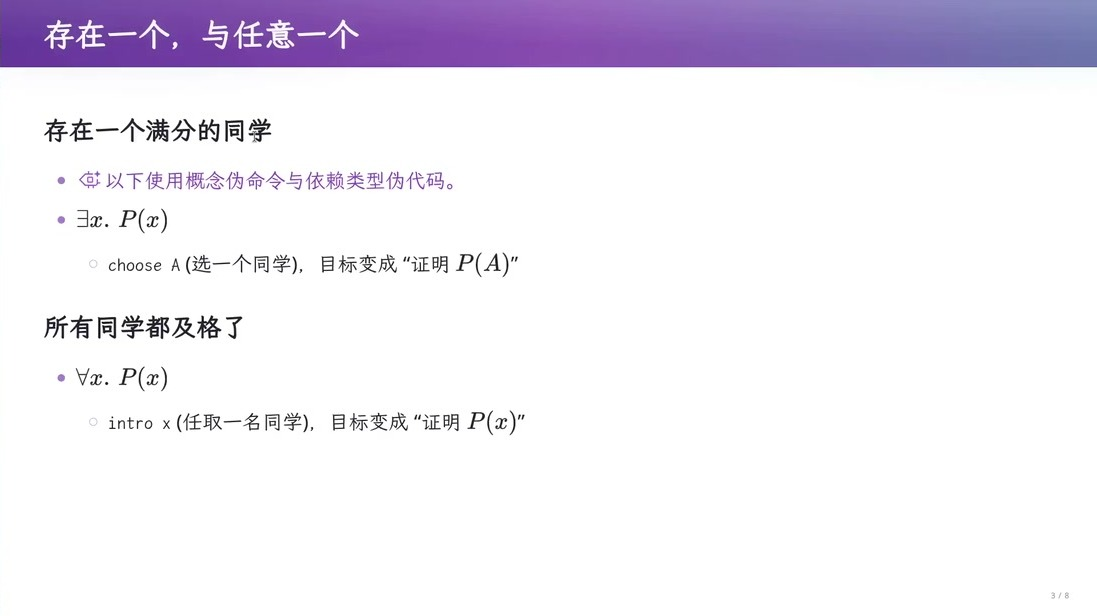
\includegraphics[width=0.86\textwidth]{figures/fig29_tactic_exists_forall.jpg}
\caption{存在量词与全称量词规则：存在命题 $\exists x.\, P(x)$ 的 \texttt{choose A} 见证选取与全称命题 $\forall x.\, P(x)$ 的 \texttt{intro x} 任取引入\vtag}
\label{fig:fig29_tactic_exists_forall}
\end{figure}
\srcnote{00:54:35--00:57:50}

\begin{figure}[H]
\centering
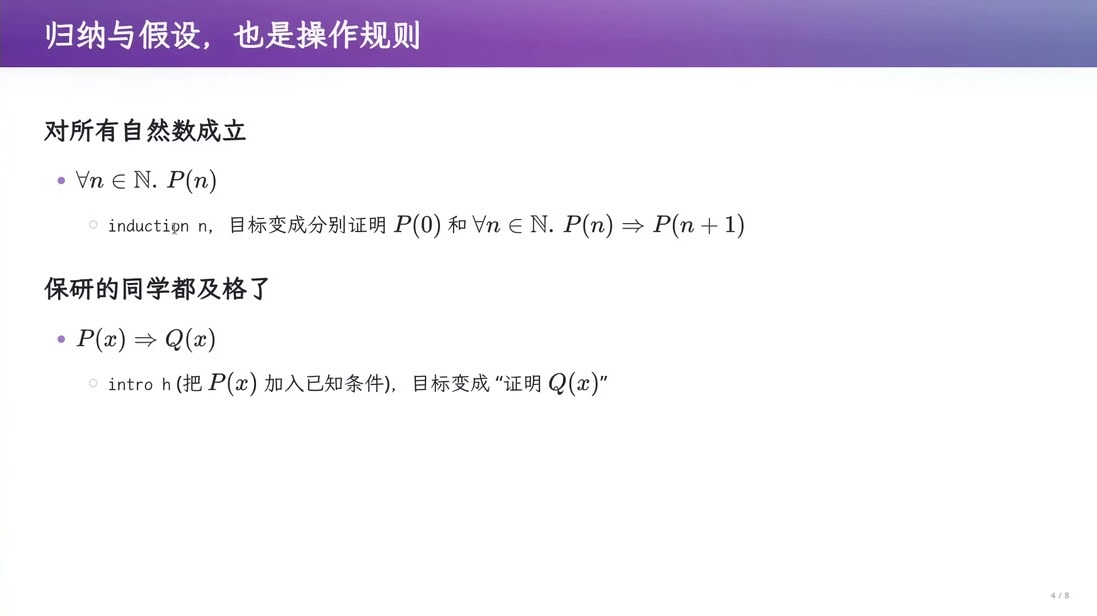
\includegraphics[width=0.86\textwidth]{figures/fig30_tactic_induction_implication.jpg}
\caption{自然数归纳与蕴含前提规则：归纳法 $\forall n \in \mathbb{N}.\, P(n)$ 的 \texttt{induction n} 拆解与蕴含 $P(x) \Rightarrow Q(x)$ 的 \texttt{intro h} 引入\vtag}
\label{fig:fig30_tactic_induction_implication}
\end{figure}
\srcnote{00:57:55--01:00:45}

\begin{enumerate}
    \item \textbf{证明存在命题 $\exists x.\, P(x)$（如“班上存在一名满分的同学”）——使用 \texttt{choose A}}：
    要证明存在某个 $x$ 满足 $P(x)$，你必须明确报出一个具体的见证人（Witness）$A$，随后待证目标就会变成“拿出同学 $A$ 确实考了满分的证据 $P(A)$”：
    \begin{equation}
    \big(\Gamma \;\vdash\; \exists x.\, P(x)\big) \;\xrightarrow{\;\texttt{choose } A\;}\; \big(\Gamma \;\vdash\; P(A)\big)
    \label{eq:tactic_choose}
    \end{equation}
    正如主讲教师在黑板上演示的：假如已知里写着“$A$ 考了 $90$ 分，$B$ 考了 $100$ 分”，如果你鲁莽地执行 `\texttt{choose A}`，这一步改写本身是合法的，但下一步目标变成 $\mathrm{Score}(A) = 100$ 后，就会因为与已知的 $\mathrm{Score}(A) = 90$ 无法匹配而卡死；你必须回溯改用 `\texttt{choose B}`，才能将目标变成 $\mathrm{Score}(B) = 100$ 并与已知完全对上。
    \item \textbf{证明全称命题 $\forall x.\, P(x)$（如“所有同学都及格了”）——使用 \texttt{intro x}}：
    要证明对任意 $x$ 性质 $P(x)$ 均成立，执行 `\texttt{intro x}` 相当于在已知上下文中引入一个\textbf{没有任何额外特殊假设的自由变量 $x_0$}（不能偷偷假定他是班里的学霸），并将目标改写为证明 $P(x_0)$：
    \begin{equation}
    \big(\Gamma \;\vdash\; \forall x: T.\, P(x)\big) \;\xrightarrow{\;\texttt{intro } x\;}\; \big(\Gamma,\, x: T \;\vdash\; P(x)\big)
    \label{eq:tactic_intro_forall}
    \end{equation}
    \item \textbf{证明蕴含命题 $P(x) \Rightarrow Q(x)$（如“保研的同学都及格了”）——使用 \texttt{intro h}}：
    要证明“若 $P(x)$ 成立则 $Q(x)$ 成立”，执行 `\texttt{intro h}` 会把前提 $P(x)$ 作为一条名为 $h$ 的新已知假设压入左侧上下文 $\Gamma$，右侧待证目标则简化为 $Q(x)$：
    \begin{equation}
    \big(\Gamma \;\vdash\; P(x) \Rightarrow Q(x)\big) \;\xrightarrow{\;\texttt{intro } h\;}\; \big(\Gamma,\, h: P(x) \;\vdash\; Q(x)\big)
    \label{eq:tactic_intro_imp}
    \end{equation}
    \item \textbf{证明自然数归纳命题 $\forall n \in \mathbb{N}.\, P(n)$——使用 \texttt{induction n}}：
    执行 `\texttt{induction n}` 会将栈顶原本的单个目标弹出，并压入两个新的待证子目标——基础情形 $P(0)$ 与归纳步骤 $\forall n \in \mathbb{N}.\, (P(n) \Rightarrow P(n+1))$：
    \begin{equation}
    \big(\Gamma \;\vdash\; \forall n \in \mathbb{N}.\, P(n)\big) \;\xrightarrow{\;\texttt{induction } n\;}\;
    \begin{cases}
    \text{子目标 1（Base）：} & \Gamma \;\vdash\; P(0) \\
    \text{子目标 2（Step）：} & \Gamma \;\vdash\; \forall n \in \mathbb{N}.\, \big(P(n) \Rightarrow P(n+1)\big)
    \end{cases}
    \label{eq:tactic_induction}
    \end{equation}
\end{enumerate}

% =========================================================================
% SECTION 7
% =========================================================================
\section{命题即类型，证明即程序：Curry--Howard 同构与依赖类型递归}

\subsection{Curry--Howard 同构：把数理逻辑推导变成“类型体操”}

前面我们看到，在 Proof Assistant 里写证明就像是操控一个状态机工作台。但真正让计算机科学家拍案叫绝、被主讲教师誉为“人类文明真正的高光时刻之一”的理论发现，是揭示了\textbf{数理逻辑（Logic）与程序设计语言类型系统（Type Systems）之间存在着严丝合缝的同构关系}——这就是著名的 \textbf{Curry--Howard 同构（Curry--Howard Correspondence / Isomorphism）}（对应配图）：
\begin{center}
\textbf{命题即类型（Propositions as Types），证明即程序（Proofs as Programs）！}
\end{center}

\begin{figure}[H]
\centering
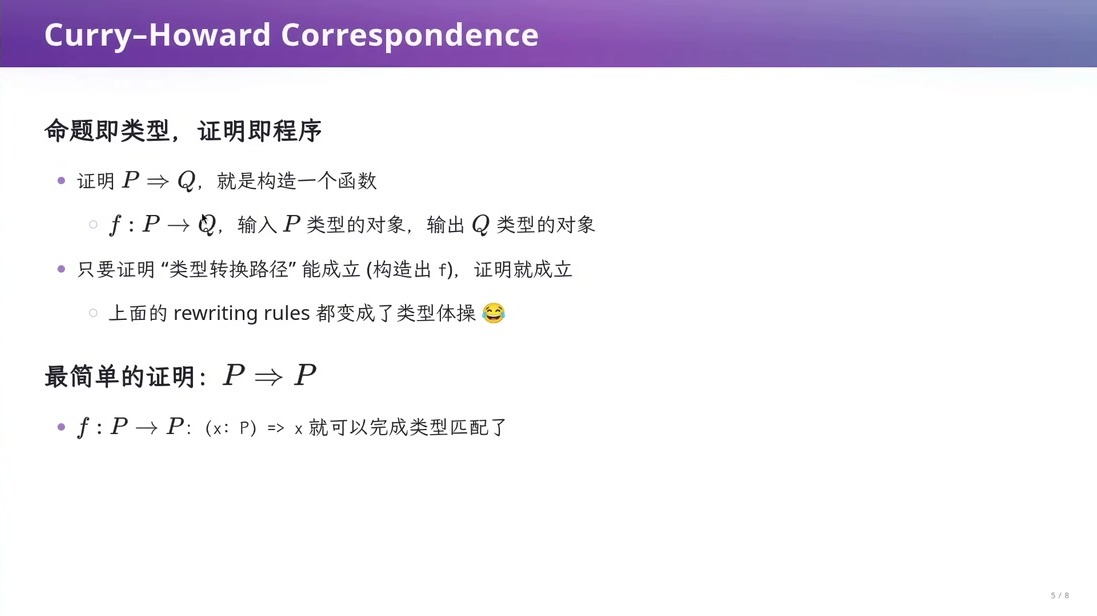
\includegraphics[width=0.88\textwidth]{figures/fig31_curry_howard_correspondence.jpg}
\caption{Curry--Howard Correspondence：命题对应类型，证明对应构造该类型对象的程序，最简单的重言式 $P \Rightarrow P$ 对应恒等函数 \texttt{(x: P) => x}\vtag}
\label{fig:fig31_curry_howard_correspondence}
\end{figure}
\srcnote{01:00:50--01:07:25}

在 Curry--Howard 同构下，任何一个逻辑命题 $P$ 都被直接看作编程语言中的一个\textbf{类型（Type）}，而命题 $P$ 的一个证明（Proof），就是属于类型 $P$ 的一个\textbf{程序对象/值（Term / Value）}。判断命题 $P$ 是否被正确证明，等价于交给编译器做\textbf{静态类型检查（Type Checking）}：只要你能不靠强制类型转换（No \texttt{unsafe} cast）、仅用合法的语言构造子写出一个类型为 $P$ 的表达式（即证明类型 $P$ 是非空的/Inhabited），命题 $P$ 就得到了证明！

具体而言，要证明蕴含命题 $P \Rightarrow Q$，在程序世界里就是要实现一个\textbf{从类型 $P$ 到类型 $Q$ 的纯函数 $f: P \to Q$}：只要调用者给它传入一个类型为 $P$ 的证明对象 $x: P$，函数 $f(x)$ 就能构造并返回一个类型为 $Q$ 的证明对象！

看一个最简单的例子：如何证明重言式 $P \Rightarrow P$（“由 $P$ 可推出 $P$”）？在程序中，它对应的类型是函数类型 $P \to P$，而它的证明就是一行连小学生都能看懂的\textbf{恒等函数（Identity Function）}：
\begin{equation}
\mathrm{id}_P \;:\; P \to P, \qquad \mathrm{id}_P \;\equiv\; (\texttt{x: P}) \Rightarrow \texttt{x}
\label{eq:curry_howard_identity}
\end{equation}
因为输入参数 `\texttt{x}` 的类型已经是 $P$，直接把 `\texttt{x}` 原封不动地 `\texttt{return}` 回去，返回值类型自然也是 $P$，类型检查瞬间通过！

更进一步，前一节介绍的四个逻辑量词与连接词操作，在依赖类型论（Dependent Type Theory，如 Lean 与 Coq 所采用的构造演算 Calculus of Constructions）中都有完全精确的程序构造对应（对应配图 与对应汇总表）：

\begin{figure}[H]
\centering
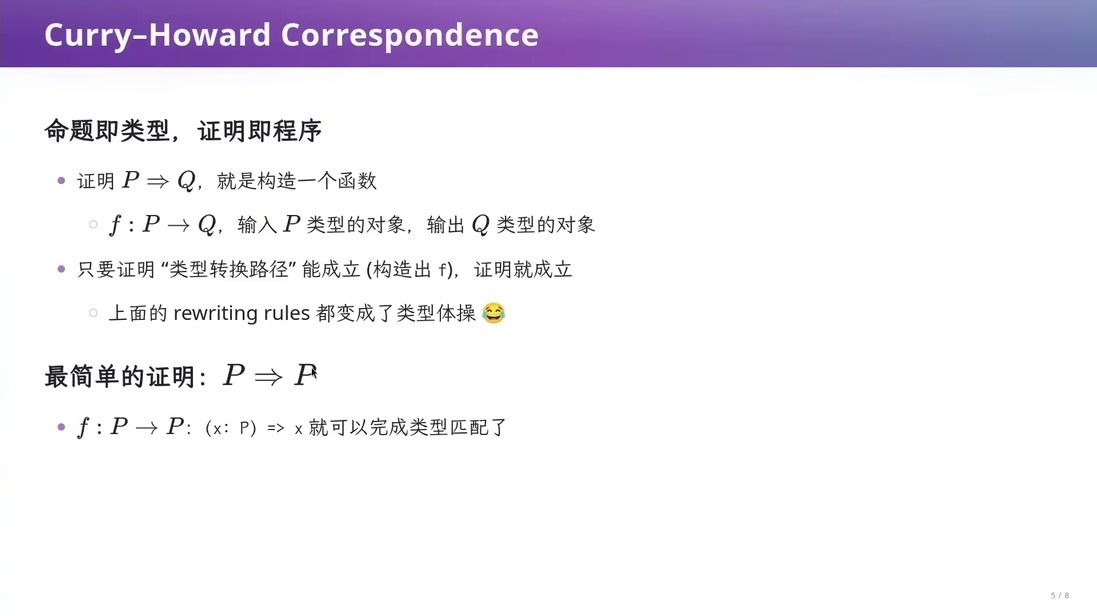
\includegraphics[width=0.88\textwidth]{figures/fig32_proof_construction_choose_intro.jpg}
\caption{证明的构造即填入缺失的程序：\texttt{Choose A} 对应构造二元组 \texttt{[A, p]}，\texttt{Intro H} 对应构造高阶函数 \texttt{(h: H) => body(h)}\vtag}
\label{fig:fig32_proof_construction_choose_intro}
\end{figure}
\srcnote{01:07:30--01:07:50}

\begin{table}[H]
\centering
\caption{Curry--Howard 同构下数理逻辑与依赖类型程序设计的完整对应字典}
\label{tab:curry_howard_dict}
\begin{tabular}{p{2.7cm}p{3.3cm}p{4.3cm}p{3.6cm}}
\toprule
\textbf{数理逻辑概念} & \textbf{程序设计/类型论概念} & \textbf{证明构造（Introduction）} & \textbf{证明使用（Elimination）} \\
\midrule
命题 $P$ & 类型 $P$ & 构造类型为 $P$ 的对象 & 读取/解构对象 \\
证明 $p$ 满足 $P$ & 表达式类型标注 $p : P$ & 通过静态类型检查 & 参与运算 \\
蕴含 $P \Rightarrow Q$ & 函数类型 $P \to Q$ & $\lambda (h: P).\, \mathrm{body}(h)$（\texttt{intro h}） & 函数调用 $f(p)$（\texttt{apply f}） \\
合取 $P \land Q$ & 积类型（二元组）$P \times Q$ & 配对 $\langle p, q \rangle$ & 投影 $\pi_1(z),\, \pi_2(z)$ \\
全称 $\forall x:A.\, P(x)$ & 依赖函数类型 $\Pi_{(x:A)} P(x)$ & $\lambda (x: A).\, \mathrm{body}(x)$（\texttt{intro x}） & 传入具体参数 $f(a) : P(a)$ \\
存在 $\exists x:A.\, P(x)$ & 依赖积类型 $\Sigma_{(x:A)} P(x)$ & 见证对 $[A,\, p: P(A)]$（\texttt{choose A}） & 模式匹配解包见证与证据 \\
假命题 $\bot$（False） & 空类型 $\mathsf{Empty}$（无构造子） & 不存在合法构造子 & 空模式匹配（反证法） \\
\bottomrule
\end{tabular}
\end{table}

用数学公式概括对应汇总表 中三大核心构造的同构映射即为：
\begin{equation}
[\![ P \Rightarrow Q ]\!] = [\![ P ]\!] \to [\![ Q ]\!], \qquad
[\![ \forall x:A.\, P(x) ]\!] = \prod_{x:A} [\![ P(x) ]\!], \qquad
[\![ \exists x:A.\, P(x) ]\!] = \sum_{x:A} [\![ P(x) ]\!]
\label{eq:curry_howard_pi_sigma}
\end{equation}
在公式 \eqref{eq:curry_howard_pi_sigma} 中：
\begin{itemize}
    \item 证明存在命题 $\exists x:A.\, P(x)$（对应 $\Sigma$ 类型），就是先选定一个具体对象 $A$，再提供一个函数把 $P(A)$ 的证据 $p$ 和 $A$ 打包成二元组 `\texttt{(p: P(A)) => [A, p]}`；
    \item 证明蕴含命题 $H \Rightarrow Q$，就是编写高阶函数 `\texttt{(body: (h: H) => Q) => (h: H) => body(h)}`，把在假设 $h: H$ 下构造 $Q$ 的过程封装起来。
\end{itemize}

\subsection{归纳证明就是递归程序：为什么证明助手严禁死循环递归？}

在这套对应关系中，最令人拍案叫绝的是：\textbf{数学归纳法（Mathematical Induction）在程序世界里恰好就是递归函数（Recursive Function）！}（对应配图）

\begin{figure}[H]
\centering
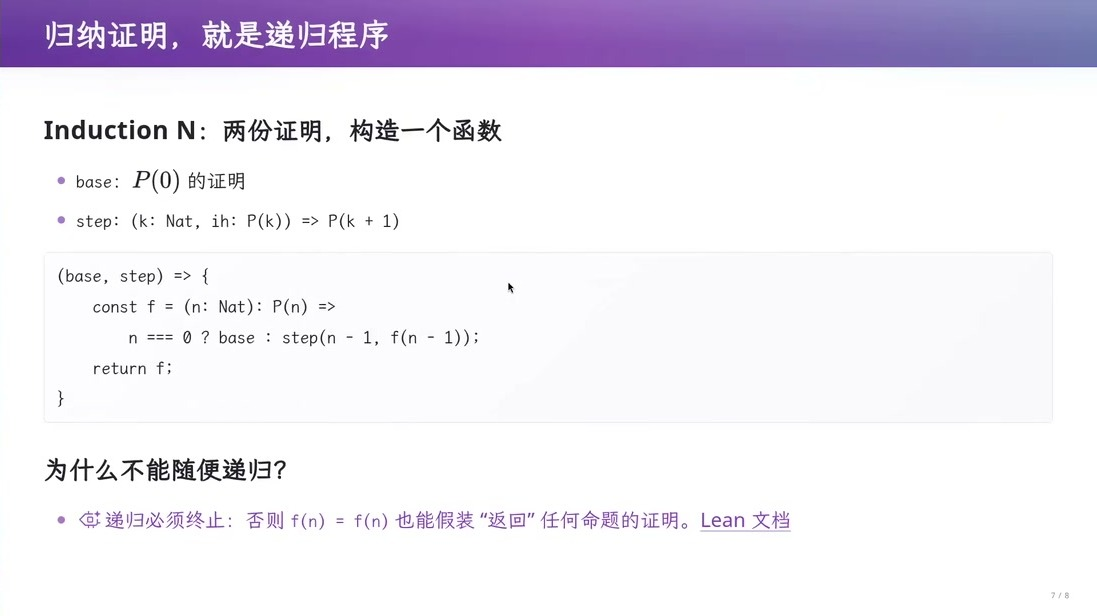
\includegraphics[width=0.88\textwidth]{figures/fig33_induction_as_recursive_program.jpg}
\caption{归纳证明就是递归程序：利用依赖类型递归函数 \texttt{f(n: Nat): P(n)} 组合 \texttt{base: P(0)} 与 \texttt{step}，以及为何必须要求递归终止\vtag}
\label{fig:fig33_induction_as_recursive_program}
\end{figure}
\srcnote{01:07:55--01:10:20}

假设我们要证明对任意自然数 $n \in \mathbb{N}$ 命题 $P(n)$ 成立（例如证明加法交换律 $\forall a, b \in \mathbb{N}.\, a + b = b + a$）。我们已经手握两份组件：
\begin{enumerate}
    \item \textbf{基础证明 \texttt{base}}：类型为 $P(0)$ 的证明对象；
    \item \textbf{归纳步函数 \texttt{step}}：类型为 $(k: \mathrm{Nat},\; \mathit{ih}: P(k)) \to P(k+1)$ 的依赖类型函数——给定任意自然数 $k$ 以及归纳假设 $\mathit{ih}: P(k)$，它能构造出 $P(k+1)$ 的证明。
\end{enumerate}
那么，如何为任意给定的自然数 $n$ 构造出 $P(n)$ 的证明？只需写一个连大一新生都会写的递归函数 \texttt{f}：
\begin{lstlisting}[language=Java, caption={自然数数学归纳法的依赖类型递归程序表示}]
// base: P(0) 的证明
// step: (k: Nat, ih: P(k)) => P(k + 1)
(base, step) => {
    const f = (n: Nat): P(n) =>
        n === 0 ? base : step(n - 1, f(n - 1));
    return f;
}
\end{lstlisting}
写成依赖类型论中的递归消去子（Eliminator）形式即为：
\begin{equation}
\mathrm{nat\_rec}(P,\, \mathit{base},\, \mathit{step},\, n) \;:\; P(n) \;=\;
\begin{cases}
\mathit{base} : P(0), & \text{若 } n = 0 \\[4pt]
\mathit{step}\big(n - 1,\; \mathrm{nat\_rec}(P, \mathit{base}, \mathit{step}, n - 1)\big) : P(n), & \text{若 } n > 0
\end{cases}
\label{eq:dependent_type_nat_rec}
\end{equation}
观察公式 \eqref{eq:dependent_type_nat_rec}：为什么说这不是普通的 JavaScript 或 TypeScript 函数？因为它的\textbf{返回值类型 $P(n)$ 依赖于输入参数 $n$ 的运行时数值}（这正是“依赖类型 Dependent Types”一词的由来）！当传入 $n = 3$ 时，$\mathrm{nat\_rec}$ 会递归展开为 $\mathit{step}(2, \mathit{step}(1, \mathit{step}(0, \mathit{base})))$，一步步从 $P(0) \to P(1) \to P(2) \to P(3)$ 算出类型为 $P(3)$ 的证明对象。

\begin{warningbox}{关键陷阱：为什么在证明助手里绝对不能随便写非终止递归？}
在普通编程语言（如 C、Python、JavaScript）中，编译器允许你写出如下无限递归函数：
\[
\texttt{const f = (n: Nat): P(n) => f(n);}
\]
如果只看局部静态类型签名：假设 `\texttt{f(n)}` 的返回类型是 $P(n)$，那么函数体直接返回 `\texttt{f(n)}` 的类型自然也是 $P(n)$！如果证明助手允许这样的无限递归通过类型检查，那就意味着\textbf{不需要任何基础证明 \texttt{base}，一行死循环 `\texttt{f(n) = f(n)}` 就能“证明”宇宙间的任何命题 $P(n)$（包括 $0 = 1$ 或黎曼猜想）}，整个逻辑系统将瞬间崩溃（陷入逻辑不一致 Inconsistency）！

因此，Lean 和 Coq 等证明助手强制要求所有参与证明的递归函数必须通过严格的\textbf{终止性检查（Termination / Structural Decreasing Check）}：如公式 \eqref{eq:dependent_type_nat_rec} 所示，每次递归调用的参数 $n - 1$ 必须在良基序（Well-founded Order）下严格小于当前参数 $n$，保证有限步内必然触底到达基础情形 $n = 0$。
\end{warningbox}

\subsection{为什么以前不早学 Proof Assistant？AI 如何改写形式化学习曲线}

既然 Proof Assistant 和 Curry--Howard 同构如此美妙，为什么以前的大学计算机课程不在大一甚至中小学普及它？主讲教师在幻灯片上幽默地写下了一句大实话（对应配图）：\textbf{“因为老师不会也学不动了啊（但小学生也许能学会呢？）”}。

\begin{figure}[H]
\centering
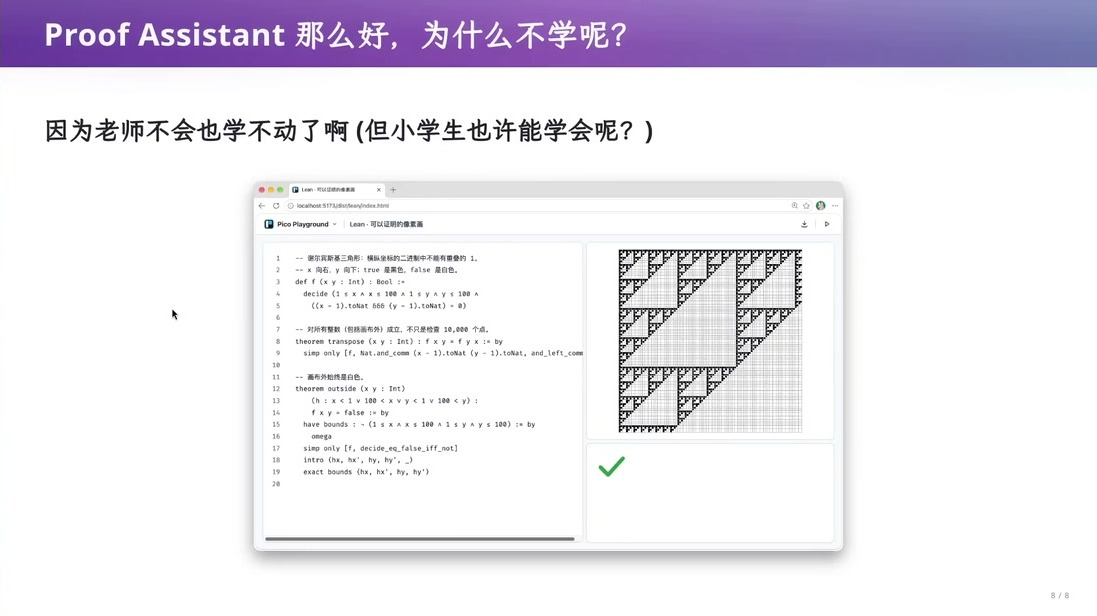
\includegraphics[width=0.88\textwidth]{figures/fig34_why_not_learn_proof_assistant.jpg}
\caption{Proof Assistant 那么好，为什么不学呢？——在 Lean 函数式语言定义中生成 $100 \times 100$ 谢尔宾斯基（Sierpinski）分形三角形并验证其数学性质\vtag}
\label{fig:fig34_why_not_learn_proof_assistant}
\end{figure}
\srcnote{01:10:25--01:12:50}

在过去，初学者哪怕想在 Lean 或 Coq 里证明一个看似再显然不过的“加法交换律 $a + b = b + a$”，都会被繁琐的归纳法拆解和陌生的 Tactic 语法折磨得寸步难行。但在今天，AI 彻底降低了这门“类型体操”的入门门槛：
\begin{enumerate}
    \item \textbf{证明助手本身就是一门优秀的函数式编程语言}：如 Lean 4 既可以在 \texttt{tactic} 模式下写数学证明，也可以直接当成纯函数式语言编写可执行代码。如对应配图 右侧所示，主讲教师将课堂上用过的 Python 汉诺塔互动游乐场（Playground）改造成了一个 Lean Playground：只需定义一个判断坐标点 $(x, y)$ 是否着色的纯函数 $f(x, y): \mathrm{Bool}$，即可在右侧 $100 \times 100$ 像素画布上实时渲染出经典的\textbf{谢尔宾斯基分形三角形（Sierpinski Triangle）}；
    \item \textbf{从“对着空白屏幕抓耳挠腮”到“看 AI 演示并审查每一步状态变化”}：在繪制出分形图案后，学习者不仅可以观察图像，还可以提出诸如“画布边界以外的所有像素是否永远为白色”之类的数学性质，让 AI 先写出 Lean 证明，自己则通过观察每一步 Tactic 如何改变左侧已知 $\Gamma$ 与右侧目标 $G$ 来建立直觉。
\end{enumerate}

% =========================================================================
% SECTION 8
% =========================================================================
\section{当 Proof 也变成一种 Tax：博士论文猜想攻关与防止“证了个寂寞”}

\subsection{课堂“鬼故事”：用不属于你的力量攻克烂尾博士论文中的 Conjecture}

在理解了 Proof Assistant 与大模型的结合原理后，主讲教师分享了一个令全场震撼的亲身经历——一个关于他自己博士论文遗留猜想（Conjecture）的“鬼故事”（对应配图）。

\begin{figure}[H]
\centering
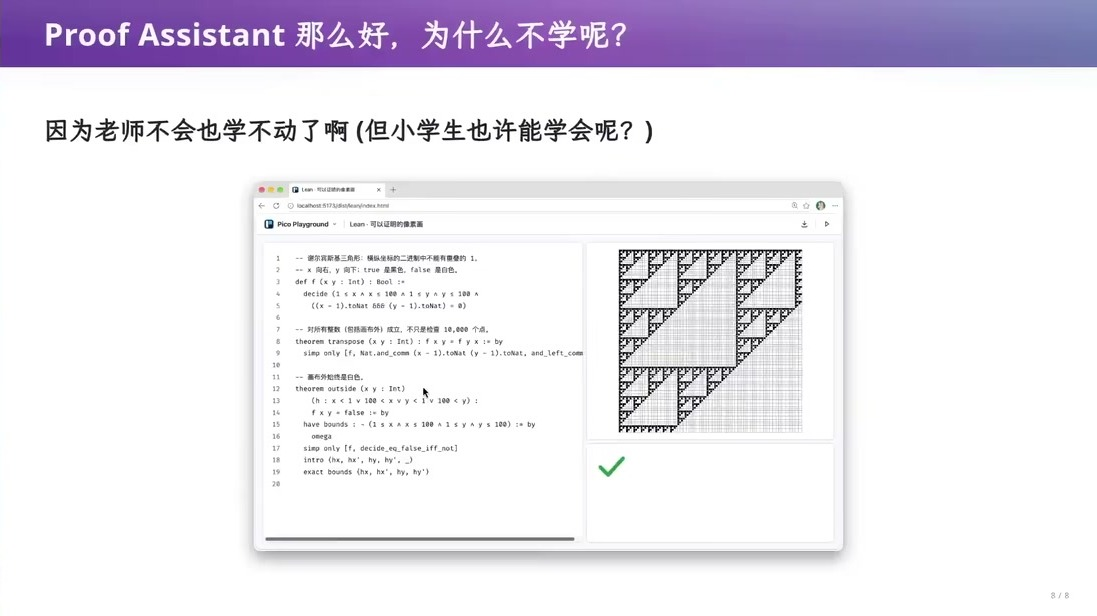
\includegraphics[width=0.88\textwidth]{figures/fig35_phd_conjecture_ghost_story.jpg}
\caption{讲一个鬼故事：借助前沿大模型与 Lean 证明助手攻克博士论文遗留猜想——“好消息：没有晚节不保！坏消息：连 proof 也变成一种 tax”\vtag}
\label{fig:fig35_phd_conjecture_ghost_story}
\end{figure}
\srcnote{01:12:55--01:16:10}

故事的背景源自主讲教师早年在知乎专栏《有没有失败的博士？》中回顾过的读博经历：当年他在研究程序执行观测与确定性重放（Deterministic Replay）时，发现了一个困扰了计算机系统界 \textbf{30年}的基本权衡（Trade-off）——如果你在程序运行时记录的信息越少（记录开销 $C_{\text{rec}}$ 越小），那么事后为了重放恢复出完整执行状态所需付出的计算开销 $C_{\text{rep}}$ 就越大；反之，要想重放快，运行时就必须记下海量日志。整整 \textbf{30年}来，人类没有任何一个系统能同时把 $C_{\text{rec}}$ 和 $C_{\text{rep}}$ 都做小（即左下角区域始终是一片空白）。

于是，他当年在博士论文里大胆立下了一个复杂性下界猜想（Conjecture）：\textbf{如果存在某种通用的程序变换与观测机制，能够对任意程序 $P$ 及其任意局部修改 $\Delta P$，在低记录开销下依然以多项式时间（Polynomial Time）恢复出关键执行性质，那么将直接推出 $\mathsf{P} = \mathsf{NP}$！}
\begin{equation}
\Big(\exists \text{ 通用低开销观测器 } \mathcal{O},\; \forall P, \Delta P:\; \mathrm{Time}\big(\mathrm{Recover}(\mathcal{O}(P, \Delta P))\big) \in \mathrm{poly}(|P|)\Big) \implies \mathsf{P} = \mathsf{NP}
\label{eq:phd_conjecture_p_np}
\end{equation}
然而，要严格证明公式 \eqref{eq:phd_conjecture_p_np}，必须同时对“任意程序 $P$”和“任意修改 $\Delta P$”做双重全称量化规约。由于当年数学功底与精力所限，他只手工给出了一个受限情形下的非形式化证明（Informal Proof），便带着遗憾将完整猜想留在了博士论文里。此后十多年间，他把那段非形式化证明反复看了上百遍，总担心哪天被人找出漏洞或者猜想被推翻而“晚节不保”。

直到最近，眼看手头的订阅额度（“重置卡”）快要过期不用就浪费了，他突然想起了这股“不属于自己的力量”：
\begin{enumerate}
    \item 首先，他把这个问题喂给最前沿的 GPT 模型。模型起初尝试了一番后曾一度放弃，声称“这个问题似乎证不出来”；
    \item 此时，主讲教师凭借自己在计算机科学领域积累的直觉与品味推了模型一把，指出了一个关键的构造方向。模型顺着这一直觉成功给出了完整的非形式化证明！
    \item 接着，他让 Claude 对这份非形式化证明做交叉审查，确认逻辑链条没有明显漏洞后，再消耗大量 Token 让智能体写下了整整 \textbf{2 万行 Lean 4 代码}，将整个主定理及其后续推论全部在 Lean 内核中形式化验证通过！
    \item 更有意思的是，当他把基于主定理顺手推出的一系列分布式计算推论交给大模型做同行评审预测时，课堂记录中 \textbf{GPT-6 给出“PODC Yes”}（达到分布式计算顶会 PODC 录用线），而 \textbf{Claude Opus 5.5 给出“PODC borderline”}（对应配图）。
\end{enumerate}

\begin{figure}[H]
\centering
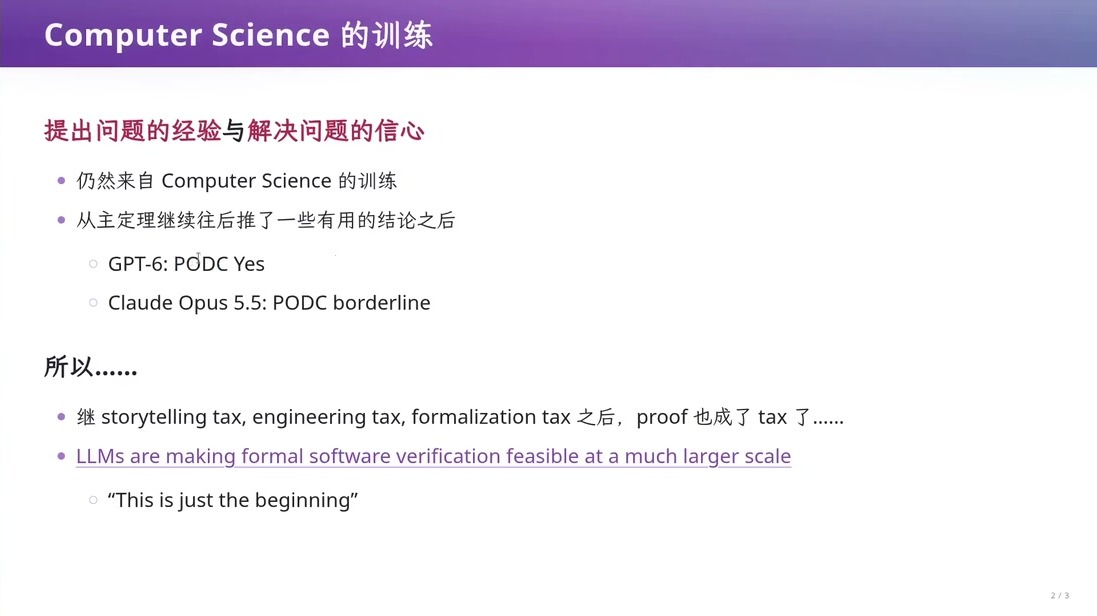
\includegraphics[width=0.88\textwidth]{figures/fig36_cs_training_and_proof_tax.jpg}
\caption{Computer Science 的训练：提出问题的经验与解决问题的信心仍来自 CS 训练，而继 storytelling、engineering、formalization tax 之后，proof 也成了 tax\vtag}
\label{fig:fig36_cs_training_and_proof_tax}
\end{figure}
\srcnote{01:16:15--01:19:55}

这一经历带来了双重的震撼（对应配图）：
\begin{itemize}
    \item \textbf{不变的内核}：\textbf{提出好问题的经验与解决问题的直觉信心，依然来自扎实的 Computer Science 训练}。如果不知道什么问题在系统领域沉淀了 30年、不知道在模型卡壳时往哪个方向推一把、不知道主定理证完后还能接着推出哪些有价值的推论，就算给你再强的模型也无从下手。
    \item \textbf{剧变的成本（Proof Tax）}：在本课程前面的章节中，我们已经相继见证了 \textbf{Storytelling Tax}（把想法包装成漂亮论文叙事的成本）、\textbf{Engineering Tax}（写代码搭系统做实验的成本）和 \textbf{Formalization Tax}（提炼数学符号定义的成本）被大模型一一碾平；而今天，\textbf{连曾经被视为人类顶尖数学智慧象征的“定理证明（Proof）”本身，也开始变成一种只需消耗算力与 Token 即可缴纳的 \texttt{Proof Tax}}！正如几天前 Anthropic 与 Theorem 发布的合作报告《LLMs are making formal software verification feasible at a much larger scale》所展示的那样：他们利用模型为一整套运行在 64MB RAM 上的工业固件及一百多个开源库在 RISC-V 汇编层面证明了免崩溃安全性质，并宣告 \textit{``This is just the beginning''}。
\end{itemize}

\subsection{如何防止形式化验证变成“证了个寂寞”？}

当构造 2 万行 Lean 证明变得轻而易举时，一个更加尖锐的工程问题立刻浮出水面：\textbf{既然人类不可能逐行去读完模型生成的 2 万行 Lean 证明，我们怎么知道模型证明的定理真的对应我们现实世界里的意图，而不是“证了个寂寞”（Vacuous Truth）？}（对应配图）

\begin{figure}[H]
\centering
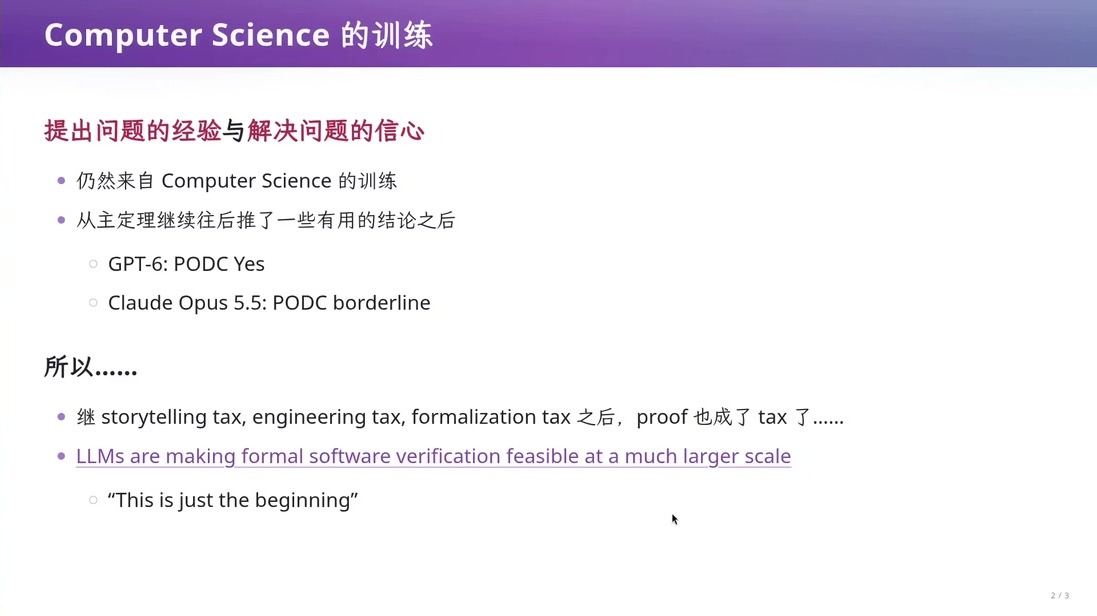
\includegraphics[width=0.88\textwidth]{figures/fig37_formalization_executable_testable.jpg}
\caption{剩下的问题——模型如何和人类世界对齐：利用形式化规约的“可执行性”与“可测试性”防止验证变成“证了个寂寞”\vtag}
\label{fig:fig37_formalization_executable_testable}
\end{figure}
\srcnote{01:20:00--01:23:15}

在历史上和大模型实践中，这类“证了个寂寞”的笑话屡见不鲜：
\begin{itemize}
    \item \textbf{通过阉割功能换取安全性质}：比如你要求证明银行转账系统的“账户余额永远非负（$\mathit{balance} \ge 0$）”，模型为了省事，把所有转账操作都实现成了 `\texttt{no-op}`（原地不动，一分钱也不转）。它的余额确实永远非负，证明也百分之百通过了 Lean 内核检查，但它根本没有实现转账功能！
    \item \textbf{在定义或前提中夹带私货（Vacuous Premise）}：比如曾有人声称用很长的形式化脚本证明了 $\mathsf{P} \neq \mathsf{NP}$ 或 $\mathsf{P} = \mathsf{NP}$，结果别人仔细检查其底层定义时才发现，他在前置定义里不小心把问题限制到了一个极其狭窄的平凡子集上，或者前提条件本身永假（$\mathsf{False} \implies Q$ 在逻辑上永远为真）！
\end{itemize}

为什么会出现这种脱节？因为软件工程始终存在两道跨越不同世界的鸿沟：
\begin{equation}
\underbrace{\text{Intent（人类意图）}}_{\text{心理/业务世界}}
\xrightarrow{\text{Gap 1: Autoformalization}}
\underbrace{\text{Spec } \Phi}_{\text{形式规约}}
\xrightarrow{\text{Gap 2: } \Pi \vdash C \models \Phi}
\underbrace{\text{Impl } C}_{\text{系统实现}}
\label{eq:intent_spec_impl_alignment}
\end{equation}
证明助手的 Kernel 只能以铁面无私的确定性替我们把守右边的 \textbf{Gap 2}（甚至如果形式化定理与真实 C 代码是分开写的两份文件，还需要检验两者之间的对应关系）；至于左边的 \textbf{Gap 1}——即那段形式化规约 $\Phi$ 到底有没有写错定义、有没有歪曲人类的真实意图——证明助手自己是无法替人类判断的！

\begin{practicebox}{工程方法论：如何检验形式化规约 $\Phi$ 没有“证了个寂寞”？}
正如主讲教师在对应配图 中所总结的，\textbf{形式化规约本身也是程序，因此形式化既可以执行（Executable），也可以测试（Testable）！}为了建立对形式化规约 $\Phi$ 的信心，我们必须构建双向对齐测试：
\begin{enumerate}
    \item \textbf{完备性/活性正例测试（Positive Liveness Traces）}：拿出一批人类熟知的、合法的业务执行轨迹 $\{ \tau^+_1, \tau^+_2, \dots \}$（例如正常的存款、扣款、成功转账序列），放入形式化模型 $\Phi$ 中直接模拟运行，断言它们\textbf{全部被规约允许通过}（防止模型把系统写成什么都不干的死锁状态机）；
    \item \textbf{健全性/反例变异测试（Negative Mutation / Fault Injection Traces）}：故意构造一批有 Bug 的错误实现或非法轨迹 $\{ \tau^-_1, \tau^-_2, \dots \}$（例如超额透支、双花攻击、并发交错写坏数据），送入规约 $\Phi$ 检查，断言它们\textbf{全部被规约无情拒绝}（防止规约写得过于宽松或前提恒假）。
\end{enumerate}
只有通过了正反双向的“规约测试”，我们才能确信证明助手所守护的那座数学大厦，真正建立在符合人类意图的基石之上。
\end{practicebox}

% =========================================================================
% SECTION 9
% =========================================================================
\section{携带证明的软件与没有银弹的未来：PCC、Autoformalization 与 System II}

\subsection{三十年回响：携带证明的代码（Proof-Carrying Code，OSDI'96 Best Paper）}

一旦大模型把“构造形式化证明”的边际成本降低几个数量级，未来整个软件工业的交付与运行形态会发生怎样的质变？为了回答这个问题，主讲教师翻出了一篇发表于整整 \textbf{30年}前的传奇论文——George C. Necula 与 Peter Lee 在 \textbf{OSDI 1996} 上斩获最佳论文奖（Best Paper Award）的《Safe Kernel Extensions Without Run-Time Checking》，以及他们在次年（\textbf{97年}）POPL 大会上进一步系统化的《Proof-Carrying Code》（对应配图）。

\begin{figure}[H]
\centering
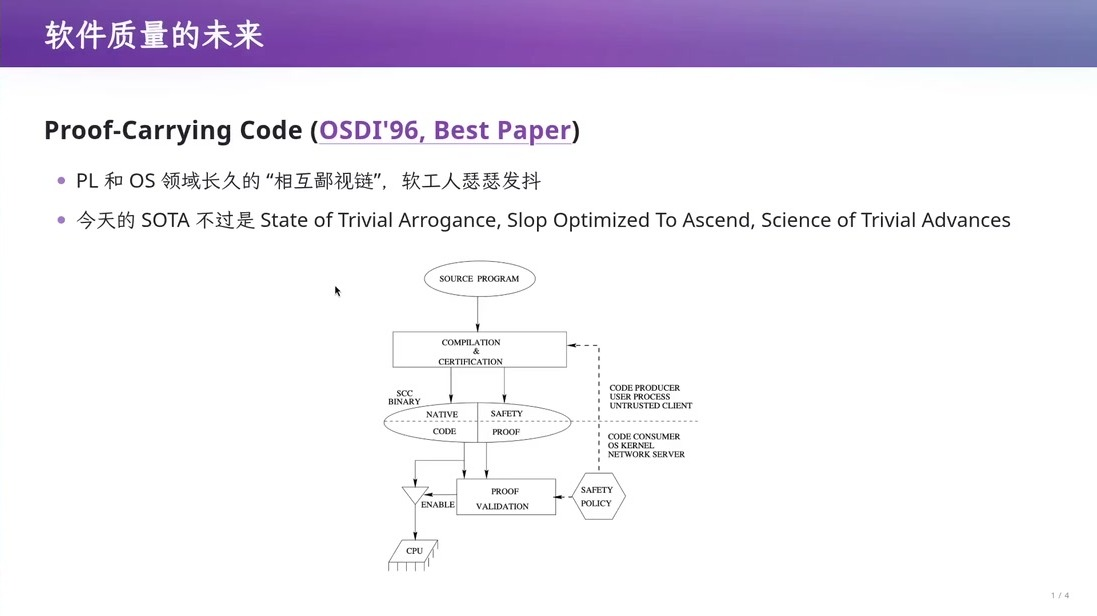
\includegraphics[width=0.88\textwidth]{figures/fig38_proof_carrying_code.jpg}
\caption{软件质量的未来：Proof-Carrying Code（OSDI'96 Best Paper）架构图，以及对 PL/OS 领域鄙视链与“SOTA”乱象的幽默解构\vtag}
\label{fig:fig38_proof_carrying_code}
\end{figure}
\srcnote{01:23:20--01:29:05}

在操作系统中（正如今天的 Linux \textbf{eBPF} 子系统），应用程序常常希望把一段不可信的扩展代码（Untrusted Kernel Extension，如网络包过滤器）直接注入操作系统内核态运行，以消除用户态与内核态切换的昂贵开销。但内核凭什么敢直接运行外来代码而不怕它把内核内存写坏或陷入死循环？

Necula 与 Lee 提出的 \textbf{携带证明的代码（Proof-Carrying Code，PCC）}给出了一个极其优雅的责任切分架构（对应配图 下方框图）：
\begin{equation}
\underbrace{\text{Code Producer（代码提供方/AI）}}_{\text{编译代码 } C \text{ 并耗费算力构造证明 } \pi}
\;\xrightarrow{\;\text{交付二元组 }(C, \pi)\;}\;
\underbrace{\text{Code Consumer（内核/接收方）}}_{\text{运行极速 }\mathrm{Verify}(\mathrm{VCGen}(C, \Phi_{\text{safe}}),\, \pi) = \mathsf{true}}
\label{eq:pcc_architecture}
\end{equation}
如公式 \eqref{eq:pcc_architecture} 所示：
\begin{itemize}
    \item \textbf{代码消费方（Code Consumer，如操作系统内核）}制定安全策略 $\Phi_{\text{safe}}$（如“绝不越界访问内存、绝不除零、必须在有限步内返回”），它\textbf{完全不需要信任代码作者，也不需要信任编译器的质量}；
    \item \textbf{代码生产方（Code Producer）}在交付二进制代码 $C$ 的同时，必须附带一份针对安全验证条件 $\mathrm{VCGen}(C, \Phi_{\text{safe}})$ 的形式化数学证明对象 $\pi$；
    \item 接收方收到 $(C, \pi)$ 后，只需运行一个极简、极快的形式化证明检验器（Proof Validator / Kernel）。因为“寻找证明很难，但检查证明极快”，一旦检验通过（$\mathrm{Verify} = \mathsf{true}$），内核就可以零运行时检查开销（Zero Run-Time Checking Overhead）地全速执行这段代码！
\end{itemize}

展望生成式软件工程的未来，当 Proof Tax 被大模型大幅降低后，PCC 将迎来真正的文艺复兴：未来的程序员或架构师在代码中写下的每一条 `\texttt{assert(invariant)}`（例如平衡树旋转后的父子指针断言），不仅可以在测试时作动态检查，\textbf{编译器还会直接调用背后的推理模型，自动为每一条 \texttt{assert} 生成对应的 Lean/Coq 形式化证明对象 $\pi$；任何无法被证明永真的 \texttt{assert} 都将直接导致编译拒绝}！届时，整套软件可靠性教科书都将被彻底改写。

主讲教师还顺带调侃了编程语言（PL）与操作系统（OS）两大社区长久以来的“相互鄙视链”——PL 学者总觉得自己早就提出了优雅的理论（如 Hoare 逻辑与 Curry--Howard 同构），看不上 OS 学者把已有理论组装应用就能拿最佳论文；而 OS 学者则只看重真实系统里管不管用，嫌弃 PL 学者整天造些没人用的屠龙之技。唯有读懂了这些跨越数十年的先驱工作，我们才能对当下论文界动辄宣称的 \textbf{“SOTA”（State of the Art）}保持一份清醒与幽默。主讲教师在幻灯片上为滥用的“SOTA”给出了三个辛辣的戏谑展开（对应配图）：
\begin{itemize}
    \item \textbf{S}tate \textbf{o}f \textbf{T}rivial \textbf{A}rrogance（琐碎傲慢之态）
    \item \textbf{S}lop \textbf{O}ptimized \textbf{T}o \textbf{A}scend（为刷榜升天而优化的泡沫）
    \item \textbf{S}cience \textbf{o}f \textbf{T}rivial \textbf{A}dvances（微不足道进展之科学）
\end{itemize}

\subsection{There Is No Silver Bullet：Autoformalization 的固有边界}

那么，既然形式化证明与大模型结合如此强大，它是不是能解决软件工程的一切问题？主讲教师再次引出了 Fred Brooks 的不朽名言——\textbf{“没有银弹（There Is No Silver Bullet）”}（对应配图 与对应配图）。

\begin{figure}[H]
\centering
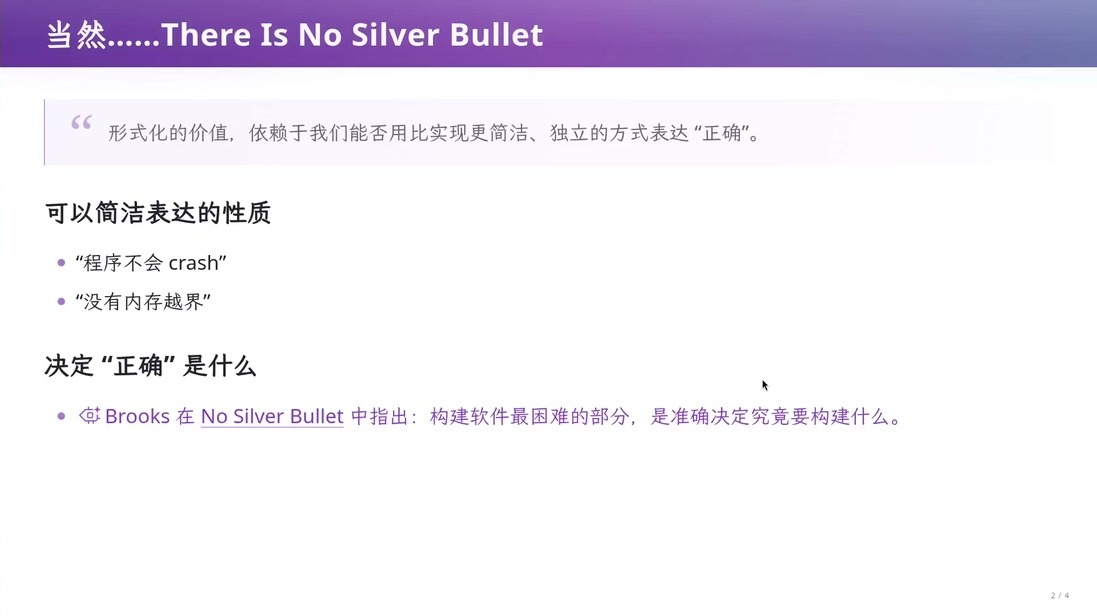
\includegraphics[width=0.86\textwidth]{figures/fig39_no_silver_bullet_formalization.jpg}
\caption{当然……There Is No Silver Bullet：形式化的价值依赖于能否用比实现更简洁、独立的方式表达“正确”\vtag}
\label{fig:fig39_no_silver_bullet_formalization}
\end{figure}
\srcnote{01:29:10--01:31:10}

\begin{figure}[H]
\centering

\includegraphics[width=0.86\textwidth]{figures/fig40_autoformalization_hard_cases.jpg}
\caption{Autoformalization 也有困难的案例：“领导满意的教务系统”与“用户满意的折叠屏关闭特效”等主观意图\vtag}
\label{fig:fig40_autoformalization_hard_cases}
\end{figure}
\srcnote{01:31:15--01:33:15}

为什么没有银弹？因为\textbf{形式化方法的全部价值，都建立在“我们能否用一种比具体代码实现更简洁、更独立的方式表达什么是正确”这一前提之上}！
\begin{itemize}
    \item \textbf{适合形式化的性质（规约远比实现简洁）}：例如“程序绝不发生内存越界崩溃”“所有数组访问满足 $0 \le i < \mathit{len}$”“并发事务绝不出现双提交矛盾”。这些规约往往只有短短几行公式，却能约束几十万行复杂的底层实现。
    \item \textbf{极难甚至无法形式化的需求（Autoformalization 的深水区）}：把非形式化的人类自然语言需求翻译为形式化数学规约的过程称为\textbf{自动形式化（Autoformalization）}。主讲教师给出了两个令所有形式化方法瞬间失效的真实场景（对应配图b）：
    \begin{enumerate}
        \item \textbf{“我要一个领导满意的教务系统”}：请问什么叫“领导满意”？你怎么在 Lean 4 里定义 $\mathrm{LeaderSatisfied}(\mathit{sys})$？领导也许根本不在乎高并发选课吞吐量，甚至不在乎偶尔的报错，他在乎的是向上汇报时数据大屏（Dashboard）够不够气派！
        \item \textbf{“我要一个用户满意的折叠屏关闭特效”}：比如折叠屏手机合上时，窗口伴随毛玻璃渐变平滑收拢并无缝切换到外屏。什么叫“自然、舒适、符合直觉预期”？你可以用形式化指标考核帧率 $\ge 120\,\mathrm{fps}$、延迟 $\le 8\,\mathrm{ms}$，但满帧低延迟的僵硬动画依然可能让用户觉得难受——因为“舒适感”植根于人类由生物化学驱动（Chemical-driven）的感官与心理共情世界！
    \end{enumerate}
\end{itemize}
正如 Brooks 在《No Silver Bullet》中深刻指出的：\textbf{构建软件最困难的部分，从来不是如何把既定规格编码实现出来，而是准确决定究竟要构建什么（Deciding precisely what to build）}。对于折叠屏动效或复杂业务系统，用户和领导甚至在看到并亲手把玩可交互原型（Prototype）之前，自己脑子里都不清楚真正想要什么！因此，当形式化证明能力越来越强时，软件工程的核心矛盾并不会消失，而是进一步向前移动到 \textbf{Intent $\leftrightarrow$ Spec} 的对齐闭环上——快速原型、探索性测试与真实人类的迭代反馈，永远是决定“我们究竟应当证明什么”的指南针。

\begin{importantbox}{生成式软件工程的新常态：当重心从 Spec $\leftrightarrow$ Impl 前移到 Intent $\leftrightarrow$ Spec}
随着大模型将代码编写（Engineering Tax）与形式化定理证明（Proof Tax）的成本大幅拉低，软件质量保障的主战场正在发生历史性迁移：通过 Proof-Carrying Code（携带证明的代码），未来编译器可以自动核验代码符合形式化规约 $\Phi$；但“形式化规约 $\Phi$ 是否真正符合人类主观意图（Intent）”却不存在银弹（No Silver Bullet）。掌握可执行规约测试、快速原型迭代与双向反馈设计，将成为 AI 时代软件工程师最核心的竞争力。
\end{importantbox}

\subsection{课堂终极思辨：关于人类 System II、随机错误注入与创造力的“暴论”}

在课程的最后三分钟，主讲教师抛出了一个极具冲击力的哲学猜想（课堂上戏称为“暴论”，对应配图）：

\begin{figure}[H]
\centering
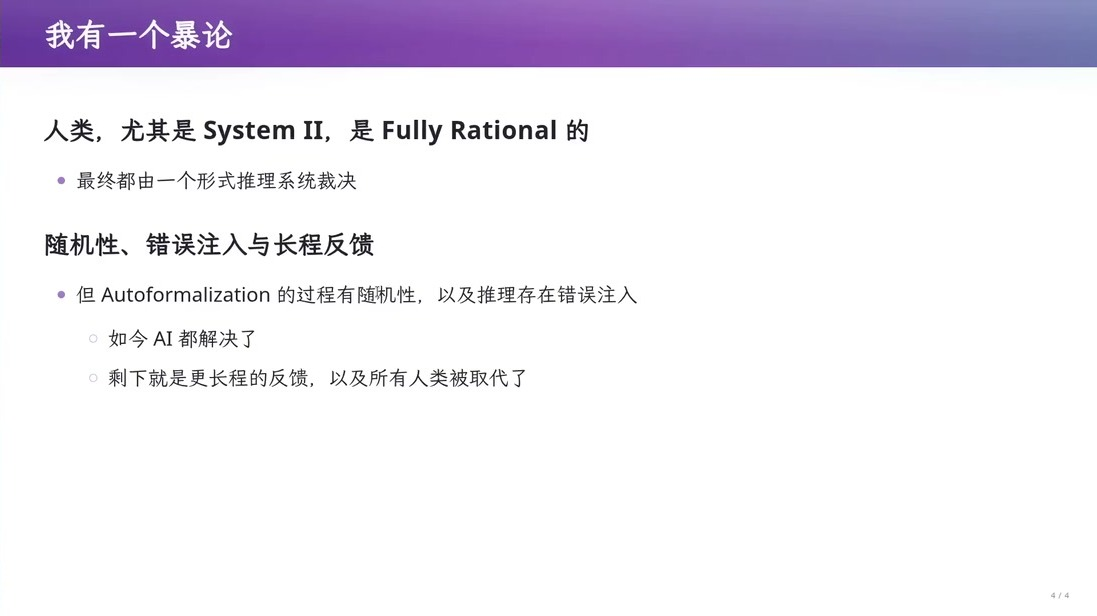
\includegraphics[width=0.88\textwidth]{figures/fig41_system2_rationality_hypothesis.jpg}
\caption{课堂思辨（“我有一个暴论”）：人类负责慢思考的 System II 本质上由形式推理系统裁决，而所谓的“灵感与创新”源自 Autoformalization 的随机性与推理错误注入\vtag}
\label{fig:fig41_system2_rationality_hypothesis}
\end{figure}
\srcnote{01:33:20--01:35:09}

人们常常浪漫地认为，人类的创造力（比如写出有创见的论文、讲出富有启发性的课程）是某种不可言喻的天赋灵光。但如果从计算与形式化系统的视角冷酷地剖析人类大脑中负责审慎慢思考的 \textbf{System II}（Kahneman 双系统理论中的理性推理系统），它或许可以被建模为一个\textbf{由价值打分网络（Grounding Network）耦合确定性形式推理系统（Formal Reasoning System）的混合架构}：
\begin{equation}
\text{Human System II Output} \;\approx\; \mathrm{FormalReasoner}\Big(\mathrm{Autoformalize}_{\text{noisy}}(\text{Environment}, \xi_{\text{rand}}),\; \epsilon_{\text{error}}\Big)
\label{eq:system2_hypothesis}
\end{equation}
在公式 \eqref{eq:system2_hypothesis} 所示的假说中，为什么人类看起来既有理性又有难以预测的“创造力”？
\begin{enumerate}
    \item \textbf{终局裁决是完全理性的形式推理}：当人类真正在做严密数学推导或逻辑决策时，底层依赖的依然是类似形式推理系统的确定性演进；
    \item \textbf{感知形式化过程中的随机性（$\xi_{\text{rand}}$）}：人类把外部物理与社会环境投射（Autoformalize）为内部心智表征的过程带有强烈的随机性与情绪波动——今天心情好觉得这个方案行，明天换个语境又觉得不行；
    \item \textbf{推理过程中的错误注入（$\epsilon_{\text{error}}$）}：人类大脑在长链条推理中不可避免地会发生算错、记混或逻辑跳跃（Error Injection）。正是这些偶然的推理偏差，把思维轨迹意外地推向了原本确定性搜索不会踏足的未知分支，事后一旦歪打正着发现了新结构，就被我们事后合理化地赞美为“灵光一闪的创新”！
\end{enumerate}

如果这一猜想成立，那么当 AI 不仅彻底掌握了形式化世界（Formal World）的严密推导，还在不断补齐自动形式化（Autoformalization）与长程现实反馈（Long-horizon Grounding Feedback）的最后拼图时，软件工程乃至人类智识活动的图景都将迎来前所未有的重塑。而在这一天真正到来之前，本讲留给每一位软件工程学习者的核心功课依然明确而坚定：\textbf{主动去体验和驾驭那些超出个人手工能力边界的AI与形式化力量，将架构设计、问题定义与双向反馈核验沉淀为我们自己不可替代的工程内核。}

% =========================================================================
% SUMMARY & FORMULAS
% =========================================================================
\newpage
\section*{全讲核心公式与知识体系速查表}

\begin{table}[H]
\centering
\caption{第 12 讲《软件质量保障 (2)》核心方法论与数学公式汇总}
\label{tab:lecture12_summary}
\begin{tabular}{p{3.4cm}p{5.5cm}p{5.5cm}}
\toprule
\textbf{模块 / 范式} & \textbf{核心形式化表达} & \textbf{工程意义与代表工具} \\
\midrule
SSOT 测试注册表 & $\mathcal{R}_{\text{doc}} \setminus \mathcal{T}_{\text{repo}} = \emptyset \;\land\; \mathcal{T}_{\text{repo}} \setminus \mathcal{R}_{\text{doc}} = \emptyset$ & \texttt{docs/testing.md} 单一事实来源，杜绝未登记测试静默漏跑 \\
Hoare 三元组 & $\{P\}\; C\; \{Q\}$（部分正确性 vs. 总正确性） & 赋予程序公理化推理基础（Floyd 1967, Hoare 1969） \\
循环不变式 & $P \Rightarrow I,\; \{I \land B\}\, C\, \{I\},\; I \land \neg B \Rightarrow Q$ & 用静态有限证明概括动态任意多轮循环（如 Boyer--Moore 投票） \\
可达状态闭包 & $R^* = \bigcup_{k\ge 0} \mathrm{Post}^k(S_0),\; \mathrm{Post}(R^*) \subseteq R^*$ & 模型检查理论基石：转移封闭且不含坏状态的 $R^*$ 即为归纳不变式 \\
符号与有界模型检查 & $\mathrm{BMC}_k = I(s_0) \land \bigwedge_{i=0}^{k-1} T_i \land \bigvee_{i=0}^k \neg P(s_i)$ & BDD（1990 突破 $10^{20}$ 状态）、BMC（1999）、CEGAR 与 IC3（2011） \\
精化映射（Refinement） & $(\alpha(s), \alpha(s')) \in \to_A \;\lor\; \alpha(s) = \alpha(s')$ & 连接 TLA+ 高层协议模型（如 2PC）与底层具体系统实现的桥梁 \\
符号执行（KLEE） & $\mathrm{SAT}(\mathit{PC}_i \land \neg \sigma_i(P))$ & 按分支约束合并输入等价类（$2^{32} \to 3$ 条路径），自动求解反例 \\
基础软件定理证明 & $\mathrm{Comp}(S)=\mathrm{OK}(C) \Rightarrow \mathrm{Beh}(C) \subseteq \mathrm{Beh}(S)$ & CompCert（3 人年、4.2万行 Coq）与 seL4（25人年、20万行证明） \\
Curry--Howard 同构 & $[\![ P \Rightarrow Q ]\!] = P \to Q,\; [\![ \forall ]\!] = \Pi,\; [\![ \exists ]\!] = \Sigma$ & 命题即类型、证明即程序、数学归纳法即带终止检查的依赖类型递归 \\
携带证明的代码（PCC） & $\mathrm{Verify}(\mathrm{VCGen}(C, \Phi_{\text{safe}}), \pi) = \mathsf{true}$ & 代码提供方构造证明 $\pi$，接收方极速核验（OSDI'96 Best Paper） \\
\bottomrule
\end{tabular}
\end{table}

\end{document}
